%%%%%%%%%%%%%%%%%%%%%%%%%%%%%%%%%%%%%%%%%%%%%%%%%%
%
%
%
%
%
%%%%%%%%%%%%%%%%%%%%%%%%%%%%%%%%%%%%%%%%%%%%%%%%%%
\documentclass[a4paper,fleqn,usenatbib]{mnras}

\usepackage{ae, aecompl, amsmath, amssymb}
\usepackage{bm}           %%  bold math
\usepackage{cancel, mathptmx}
\usepackage{dcolumn}  %%  Align table columns on decimal point
\usepackage{epsfig, epsf, etoolbox}
\usepackage{fancyhdr}
\usepackage{graphicx}
\usepackage[T1]{fontenc}
%\usepackage{lscape}
\usepackage{ifthen}
\usepackage{hyperref}
\usepackage{multirow}
\usepackage{newtxtext, newtxmath}
\usepackage{pifont}% http://ctan.org/pkg/pifont
\usepackage{subfigure}
\usepackage{verbatim}

\usepackage{xcolor}
%\usepackage[square, sort, comma, numbers]{natbib}
\usepackage{threeparttable}
%\usepackage[square,sort,comma,numbers]{natbib}

\usepackage{graphicx}	% Including figure files
\usepackage{tikz}
\def\checkmark{\tikz\fill[scale=0.4](0,.35) -- (.25,0) -- (1,.7) -- (.25,.15) -- cycle;} 



%%%%%%%%%%%%%%%%%%%%%%%%%%%%%%%%%%%%%%%%%%%
%       define Journal abbreviations      %
%%%%%%%%%%%%%%%%%%%%%%%%%%%%%%%%%%%%%%%%%%%
\def\nat{Nat} \def\apjl{ApJ~Lett.} \def\apj{ApJ}
\def\apjs{ApJS} \def\aj{AJ} \def\mnras{MNRAS}
\def\prd{Phys.~Rev.~D} \def\prl{Phys.~Rev.~Lett.}
\def\plb{Phys.~Lett.~B} \def\jhep{JHEP}
\def\npbps{NUC.~Phys.~B~Proc.~Suppl.} \def\prep{Phys.~Rep.}
\def\pasp{PASP} \def\aap{Astron.~\&~Astrophys.} \def\araa{ARA\&A}
\def\jcap{\ref@jnl{J. Cosmology Astropart. Phys.}} 
\def\nar{New~A.R.} 

\newcommand{\preep}[1]{{\tt #1} }

%%%%%%%%%%%%%%%%%%%%%%%%%%%%%%%%%%%%%%%%%%%%%%%%%%%%%
%              define symbols                       %
%%%%%%%%%%%%%%%%%%%%%%%%%%%%%%%%%%%%%%%%%%%%%%%%%%%%%
\def \Mpc {~{\rm Mpc} }
\def \Om {\Omega_0}
\def \Omb {\Omega_{\rm b}}
\def \Omcdm {\Omega_{\rm CDM}}
\def \Omlam {\Omega_{\Lambda}}
\def \Omm {\Omega_{\rm m}}
\def \ho {H_0}
\def \qo {q_0}
\def \lo {\lambda_0}
\def \kms {{\rm ~km~s}^{-1}}
\def \kmsmpc {{\rm ~km~s}^{-1}~{\rm Mpc}^{-1}}
\def \hmpc{~\;h^{-1}~{\rm Mpc}} 
\def \hkpc{\;h^{-1}{\rm kpc}} 
\def \hmpcb{h^{-1}{\rm Mpc}}
\def \dif {{\rm d}}
\def \mlim {m_{\rm l}}
\def \bj {b_{\rm J}}
\def \mb {M_{\rm b_{\rm J}}}
\def \mg {M_{\rm g}}
\def \mi {M_{\rm i}}
\def \qso {_{\rm QSO}}
\def \lrg {_{\rm LRG}}
\def \gal {_{\rm gal}}
\def \xibar {\bar{\xi}}
\def \xis{\xi(s)}
\def \xisp{\xi(\sigma, \pi)}
\def \Xisig{\Xi(\sigma)}
\def \xir{\xi(r)}
\def \max {_{\rm max}}
\def \gsim { \lower .75ex \hbox{$\sim$} \llap{\raise .27ex \hbox{$>$}} }
\def \lsim { \lower .75ex \hbox{$\sim$} \llap{\raise .27ex \hbox{$<$}} }
\def \deg {^{\circ}}
%\def \sqdeg {\rm deg^{-2}}
\def \deltac {\delta_{\rm c}}
\def \mmin {M_{\rm min}}
\def \mbh  {M_{\rm BH}}
\def \mdh  {M_{\rm DH}}
\def \msun {M_{\odot}}
\def \z {_{\rm z}}
\def \edd {_{\rm Edd}}
\def \lin {_{\rm lin}}
\def \nonlin {_{\rm non-lin}}
\def \wrms {\langle w_{\rm z}^2\rangle^{1/2}}
\def \dc {\delta_{\rm c}}
\def \wp {w_{p}(\sigma)}
\def \PwrSp {\mathcal{P}(k)}
\def \DelSq {$\Delta^{2}(k)$}
\def \WMAP {{\it WMAP \,}}
\def \cobe {{\it COBE }}
\def \COBE {{\it COBE \;}}
\def \HST  {{\it HST \,\,}}
\def \Spitzer  {{\it Spitzer \,}}
\def \ATLAS {VST-AA$\Omega$ {\it ATLAS} }
\def \BEST   {{\tt best} }
\def \TARGET {{\tt target} }
\def \TQSO   {{\tt TARGET\_QSO}}
\def \HIZ    {{\tt TARGET\_HIZ}}
\def \FIRST  {{\tt TARGET\_FIRST}}
\def \zc {z_{\rm c}}
\def \zcz {z_{\rm c,0}}


\newcommand{\sqdeg}{deg$^{-2}$}
\newcommand{\lya}{Ly$\alpha$\ }
%\newcommand{\lya}{Ly\,$\alpha$\ }
\newcommand{\lyaf}{Ly\,$\alpha$\ forest}
%\newcommand{\eg}{e.g.~}
%\newcommand{\etal}{et~al.~}
\newcommand{\cii}{C\,{\sc ii}\ }
\newcommand{\ciii}{C\,{\sc iii}]\ }
\newcommand{\civ}{C\,{\sc iv}\ }
\newcommand{\SiIV}{Si\,{\sc iv}\ }
\newcommand{\mgii}{Mg\,{\sc ii}\ }
\newcommand{\feii}{Fe\,{\sc ii}\ }
\newcommand{\feiii}{Fe\,{\sc iii}\ }
\newcommand{\caii}{Ca\,{\sc ii}\ }
\newcommand{\halpha}{H\,$\alpha$\ }
\newcommand{\hbeta}{H\,$\beta$\ }
\newcommand{\oi}{[O\,{\sc i}]\ }
\newcommand{\oii}{[O\,{\sc ii}]\ }
\newcommand{\oiii}{[O\,{\sc iii}]\ }
\newcommand{\heii}{[He\,{\sc ii}]\ }
\newcommand{\nii}{N\,{\sc ii}\ }
\newcommand{\nv}{N\,{\sc v}\ }

%% From:: /cos_pc19a_npr/LaTeX/proposals/JWST/JWST_ERS/Proposal/lines.tex
%%  
\newcommand{\imw}{$i$--$W3$}
\newcommand{\imwf}{$i$--$W4$}
\newcommand{\rmwf}{$r$--$W4$}
\newcommand{\imwt}{$i$--$W2$}
\newcommand{\wtmwf}{$W3$--$W4$}
%\newcommand{\kms}{km s$^{-1}$}
\newcommand{\cmN}{cm$^{-2}$}
\newcommand{\cmn}{cm$^{-3}$}
%\newcommand{\msun}{M$_{\odot}$}
\newcommand{\lsun}{L$_{\odot}$}
\newcommand{\lam}{$\lambda$}
\newcommand{\mum}{$\mu$m}
\newcommand{\ebv}{$E(B$$-$$V)$}
%\newcommand{\heii}{\mbox{He\,{\sc ii}}}
\newcommand{\cv}{\mbox{C\,{\sc v}}}
%\newcommand{\civ}{\mbox{C\,{\sc iv}}}
%\newcommand{\ciii}{\mbox{C\,{\sc iii}}}
%\newcommand{\cii}{\mbox{C\,{\sc ii}}}
%\newcommand{\nv}{\mbox{N\,{\sc v}}}
\newcommand{\niv}{\mbox{N\,{\sc iv}}}
\newcommand{\niii}{\mbox{N\,{\sc iii}}}
%\newcommand{\oi}{\mbox{O\,{\sc i}}}
%\newcommand{\oii}{\mbox{O\,{\sc ii}}}
%\newcommand{\oiii}{\mbox{[O\,{\sc iii}]}}
\newcommand{\oiv}{\mbox{O\,{\sc iv}}}
\newcommand{\ov}{\mbox{O\,{\sc v}}}
\newcommand{\ovi}{\mbox{O\,{\sc vi}}}
\newcommand{\ovii}{\mbox{O\,{\sc vii}}}

%\newcommand{\feii}{\mbox{Fe\,{\sc ii}}}
%\newcommand{\feiii}{\mbox{Fe\,{\sc iii}}}
%\newcommand{\mgii}{\mbox{Mg\,{\sc ii}}}
\newcommand{\neii}{[Ne\,{\sc ii}]\ }
\newcommand{\neiii}{[Ne\,{\sc ii}]\ }
\newcommand{\nev}{Ne\,{\sc v}\ }
\newcommand{\nevi}{[Ne\,{\sc vi}]\ }
\newcommand{\neviii}{\mbox{Ne\,{\sc viii}}}
\newcommand{\aliii}{\mbox{Al\,{\sc iii}}}
\newcommand{\siii}{\mbox{Si\,{\sc ii}}}
\newcommand{\siiii}{\mbox{Si\,{\sc iii}}}
\newcommand{\siiv}{\mbox{Si\,{\sc iv}}}
%\newcommand{\lya}{\mbox{Ly$\alpha$}}
%\newcommand{\lyb}{\mbox{Ly$\beta$}}
\newcommand{\hi}{\mbox{H\,{\sc i}}}
\newcommand{\snine}{\mbox{[S\,{\sc ix}]}}
\newcommand{\sivi}{\mbox{[Si\,{\sc vi}]}}
\newcommand{\sivii}{\mbox[{Si\,{\sc vii}]}}
\newcommand{\siix}{\mbox{[Si\,{\sc ix}]}}
\newcommand{\six}{\mbox{[Si\,{\sc x}]}}
\newcommand{\sixi}{\mbox{[Si\,{\sc xi}]}}
\newcommand{\caviii}{\mbox{[Ca\,{\sc viii}]}}
\newcommand{\arii}{\mbox{[Ar\,{\sc ii}]}}

%%[Ar II] 6.97
%% [S IX] 1.252 μm 328 
% [Si X] 1.430 μm 351 
% [Si XI] 1.932 μm 401 
% [Si VI] 1.962 μm 167 
% [Ca VIII] 2.321 μm 128 
% [Si VII] 2.483 μm 205 
% [Si IX] 3.935 μm 303
% [Ar II] 6.97


%\snine\ at 1.252$\mu$m, \six\ at 1.430$\mu$m, \sixi\ at 1.932$\mu$m, \sivi\ at
%1.962$\mu$m, \caviii\ at 2.321$\mu$m, \sivi\ at 2.483$\mu$m \siix\ at
%3.935$\mu$m and \arii\ at 6.97$\mu$m. 
%%
%% such as [Ne ii]12.8 μm, [Ne v]14.3 μm, [Ne iii]15.5 μm, [S iii]18.7 μm and 33.48 μm, [O iv]25.89 μm and [Si ii]34.8 μm (e.g
%%
%% MIR emission lines like [NeII] and [NeV] are ..
%%
%% Also,  arXiv:astro-ph/0003457v1 
%% [NeV] 14.32um & 24.32um and [NeVI] 7.65um imply an A(V)>160 towards the NLR...
%% [NeIII]15.56um/[NeII]12.81um
%%
%% [Ne V] 14.3, 24.2 μm 97.
%% [Ne II] 12.8 μm
%% [OIV] 26μm
%%



\title[Infrared CLQs from WHT]
{Optical Properties of Quasars that have rapidly Rising and Falling Infrared flux}

\author[Bercow]
{%The RH John~S.~Bercow, MP, {\it et al.} 
Nicholas~P.~Ross$^{1}$\thanks{E-mail: npross@roe.ac.uk},   
{\bf et  al.}
%%K. E. Saavik Ford$^{2,3,4}$,  Matthew Graham$^{5}$,  Barry McKernan$^{2,3,4}$,  
%% A. Bruce ^{1}$, D. Homan ^{1}$, A. Lawrence ^{1}$, 
%\newauthor Daniel Stern$^{6}$, 
%Aaron M. Meisner$^{7,8}$, 
\\
%% List of institutions
%$^{1}$Speaker's Chair, The House of Commons, London, SW1A 0AA \\
$^{1}$Institute for Astronomy, University of Edinburgh, Royal Observatory, Blackford Hill, Edinburgh EH9 3HJ, United Kingdom \\
%$^{2}$Department of Science, BMCC, City University of New York, New York, NY 10007, USA \\
%$^{3}$Department of Astrophysics, Rose Center for Earth and Space, American Museum of Natural History, Central Park West at 79th Street, NY 10024, USA \\
%$^{4}$Graduate Center, City University of New York, 365 5th Avenue, New York, NY 10016, USA\\
%$^{5}$Cahill Center for Astronomy and Astrophysics, California Institute of Technology, Mail Code 249/17, 1200 E California Blvd, Pasadena CA 91125, USA\\
%$^{6}$Jet Propulsion Laboratory, California Institute of Technology, 4800 Oak Grove Drive, Mail Stop 169-221, Pasadena, CA 91109, USA \\
}

% These dates will be filled out by the publisher
\date{Accepted XXX. Received YYY; in original form ZZZ}
% Enter the current year, for the copyright statements etc.
\pubyear{2020}


\begin{document}
\label{firstpage}
\pagerange{\pageref{firstpage}--\pageref{lastpage}}
\maketitle

\begin{abstract}
``Changing-look'' quasars (CLQs) vary much faster than expected from
classic, thin, Shakura-Sunyaev accretion disks. Our team has recently
demonstrated that infrared-selected CLQs allow us to probe the very
central regions of quasars, including the innermost stable circular
orbit (ISCO) and potentially test predictions of General
Relativity. We have extracted a set of 21 IR-selected CLQs from the
SDSS using new data from the NEOWISE-R mission. These objects have
striking falling and rising mid-IR fluxes, but have representative
SDSS spectra from $\approx$6 to 14 years ago (rest-frame).  We propose
the first systematic study of IR-selected CLQs and request 2 dark
nights in order to reveal the recent optical spectral state of these
quasars. Our baseline expectation is that WHT spectra of the IR Risers
(Faders) will show hotter, bluer (cooler, redder) disks with larger
(smaller) EW broad lines than seen with SDSS. Likewise, WHT optical
spectra of the IR Faders will show cooler, redder disks with smaller
EW broad lines than seen by SDSS. Any departure from this expectation
will further inform us how the classical model breaks down.
\end{abstract}

% Select between one and six entries from the list of approved keywords.
% Don't make up new ones.
\begin{keywords}
keyword1 -- keyword2 -- keyword3
\end{keywords}



%%%%%%%%%%%%%%%%% BODY OF PAPER %%%%%%%%%%%%%%%%%%

\section{Introduction}
``Changing-look'' quasars (CLQs) vary much faster than expected from
classic, thin, Shakura-Sunyaev accretion disks, and lead to the
current situation that has been dubbed the ``Quasar viscosity crisis''
where the CLQs have broken standard viscous accretion disk models
\citep[e.g.][]{Lawrence2018, Antonucci2018}. Infrared (IR)
observations allow us to rule out obscuration as a cause of the
extreme variability. As we showed in \citet{Ross2018} and
\citet{Stern2018}, optical variability of IR-selected CLQs is so fast
and of such large amplitude that the driver is most likely changes in
a puffed-up, viscous inner accretion disk, close to the innermost
stable circular orbit (ISCO).

As a result, IR-selected CLQs \citep{Graham2019} allow us to
probe the innermost regions of quasars, including the ISCO, the
plunging region and to investigate predictions of General Relativity
in strong gravity. The role of IR-selection is key to revealing these
powerful probes of disks and spacetime close to the black hole.

Although extreme IR variability rules out the dust obscuration
scenario for the currently discovered CLQs, understanding what the
{\it hot dust} does, on the outer, or indeed maybe even overlapping,
edge of the BLR is crucial to understanding how central engines work
and how their photon and energy budget propagate to the nuclear
galactic regions. 

IR emission from quasars is widely believed to be produced in dusty
gas by reprocessed continuum UV emission. We have extracted a set of
$z\approx 0.3$ quasars that exhibit striking `falling' (Fig.~1; top)
and `rising' (Fig.~1; bottom) mid-IR fluxes over a period of
$\approx$4 years. In each case we have representative SDSS spectra
(see Fig.~2) from before this fade/rise and we have established that
these objects are not blazars by removing objects that would fulfil a
traditional ``radio loud'' criterion.

WHT spectra of these quasars will allow us to carry out a simple test
of the IR ``Risers'' and ``Faders''. Since IR emission is reprocessed
continuum emission from the disk, our baseline expectation (null
hypothesis) is that WHT spectra of the ``Risers'' will show hotter,
bluer disks with larger EW broad lines than seen with SDSS. Likewise,
WHT optical spectra of the ``Faders'' will show cooler, redder disks
with smaller EW broad lines than seen by SDSS. Measuring the EW in
both states is good test for SED changes where we need a larger sample
than currently available to not be limited statistically. Here we
propose the first ever systematic study of IR-selected CLQs.  We
request two dark nights in order to reveal the optical spectral
properties of these quasars.

Crucially, we have first epoch spectral data from SDSS, and thus can
perform an ``absolute'' (i.e. 1st epoch vs. 2nd epoch) measurement as
well as a ``relative'' (2nd epoch Risers vs. 2nd epoch Faders)
test. By comparing the disk luminosity between the 1st epoch SDSS
spectra and the 2nd epoch WHT spectra we will be able to constrain the
change in the accretion rate and inner disk temperature for each
quasar. This difference should be directly comparable to the magnitude
of IR rise or fall in that quasar between epochs.  Thus, we have a
strict and simple null hypothesis test. A confirmation of the null
hypothesis in our sample gives us some confidence that IR-selection of
CLQs is probing what we think it should, i.e. dusty gas beyond the
regular broadline region. Any departure from the null hypothesis
reveals a flaw in our simple expectations and a flaw in the
IR-selection criterion of CLQs. It will provide grounds for both
follow-up theoretical work and follow-up observations on a larger
sample of risers and faders. The latter will test the rate of
departure from our null hypothesis for CLQs.

As such, even if we do not observe any significant differences in the
second spectral epoch to the first, this is interesting due to the
dramatic differences in the associated infrared fluxes. Moreover, it
is currently unknown whether there are any fundamental differences
between quasars that show an increase in the MIR flux compared to
those that show a decrease.

Our sample spans a period of $\approx$6-14 years in the rest-frame
since the SDSS spectra were obtained, see Figure 3, and these objects
also generally have Eddington ratios $\approx$1\% -- 10\%. Calculating
if there has been an increase/decrease in the Eddington ratio in 2019A
will again give key insights on the mechanisms powering extremely
variable quasars.

If our hypothesis is supported by the data, we will be able to
quantify the expected variability in the IR due to optical continuum
changes. This will enable us to further investigate the relationship
between the optical continuum source and the IR source in AGN, and, in
particular how changes of the innermost accretion disk (near the ISCO)
impact AGN structures at parsec (and perhaps larger) scales.

Finally, we note that obtaining time-domain spectroscopy for
IR-variable quasars, links directly to the WEAVE science case and
observations of radio AGN and galaxies in the medium deep LOFAR
surveys and quasars detected in ESA {\it Gaia}.

%See Figure 2. 
%%	WISE J1052+1519 (Stern et al. 2018) and J1100-0053  (Ross et al. 2018) are added at the     end for comparison. 
%{\bf Also}, dust reverberation e.g. Gorjian, Shen, Barth (2017)\\
%Billy Vazquez — Reverberation Mapping of Seyfert 1s: Probing the dusty torus at 3.6 and 4.5 micron with the Spitzer Space Telescope




%%%%%%%%%%%%%%%%%%%%%%%%%%%%%%%%%%%%%%%%%%%%%%%%%%%%%%
%% 
%% 
%%         S E C T I O N    2            S E C T I O N    2            S E C T I O N    2       
%% 
%% 
%%%%%%%%%%%%%%%%%%%%%%%%%%%%%%%%%%%%%%%%%%%%%%%%%%%%%%
\section{Sample Selection and Observations}\label{sec:data} 

\subsection{IR CLQ Sample Selection}
\begin{table*}
\begin{tabular} {l  cc  cc l l}
\hline \hline
                                                 &                              &                             &                                   &                                        &                   & \\
Object Name                             & R.A.                       & Decl.                     & redshift                     & SDSS MJD                        & WHT night &  Notes\\
                                                 &                              &                             &                                   &                                        &                   & \\
\hline      
J1348+2456   &  207.092999671   &  +24.947260777   &  0.293    & 53535    & 2nd      & ROSAT source \\
%                                                 &   13:48:22.31        &  +24:56:50.13       &                                         &                                         &             &     \\ 
J1555+2119   &  238.834080827   &  +21.320782052   &  0.289    & 53557    & 2nd      & Host seen in SDSS image \\
%                                                 &  15:55:20.17         &  +21:19:14.81       &                                         &                                         &             &     \\ 
J1600+3345   &  240.013675832   &  +33.762683980    &  0.349   & 53142    &  2nd     &    \\
%                                                 &  16:00:03.28         &  +33:45:45.66        &                                        &                                         &             &     \\ 
J1601+4745   &  240.296914145   & +47.752692667     &  0.297   & 52354    &  1st      &     \\
%                                                 & 16:01:11.25          &  +47:45:09.69         &                                        &                                         &             &     \\    
J1603+1531   &  240.759453240   &  +15.532625448     &  0.346   & 53555    &   2nd    &    \\
%                                                &  16:03:02.26         &  +15:31:57.45	   &                                         &                                         &             &     \\ 
J1605+4834   &  241.283014512   &  +48.572815722     &  0.294    & 52054   &   1st    &     \\
%                                                &  16:05:07.92         &  +48:34:22.13         &                                         &                                        &            &      \\ 
J1605+2309   &  241.392222406   &  +23.163897868      &  0.316   & 53524   &   1st     &     Balmer disk emitter (??)  \\
%                                                &  16:05:34.12         &  +23:09:50.03         &                                         &                                        &             &      \\ 
J1610+1525   &  242.631737970   &   15.427023939       & 0.301     &53918    &   1st     &      \\
%                                                &  16:05:34.13         &  +15:25:37.28          &                                        &                                        &              &     \\ 
J1615+2507   &  243.910890725   &  +25.122351270     &0.284     & 53493    &  2nd      &  ROSAT source   \\
%                                               &  16:15:38.61         & +25:07:20.46          &                                        &                                         &              &        \\  
J1632+2403   &  248.238039021   &  24.055350336        &0.310    &53177     &   1st       &       \\
%                                                &  16:32:57.14         &  +24 03 19.26         &                                       &                                          &              &        \\   
J1634+1118   &  248.712924199   &  +11.313665524      &0.294   & 54585     &  1st      &          \\
%                                                & 16:34:51.10          &  +11:18:49.24         &                                        &                                          &              &           \\  
J1704+3331   & 256.104645878    &  +33.529446263     & 0.290    & 52427     &   1st    &            \\
%                                               & 17:04:25.11          &  +33:31:45.99        &                                       &                                            &             &           \\  
J1709+3421   & 257.494827595    &  +34.358145781    & 0.314    & 54586     &   1st     &          \\
%                                               & 17:09:58.75          & +34:21:29.36          &                                     &                                            &             &           \\  
J1713+2736   &  258.474381047   &  +27.607453430     & 0.298   & 52410      &  2nd      & \citet{Sheng2019} \\
%                                               &  17:13:53.84         &  +27:36:26.82         &                                       &                                          &              &      \\  
J2102-0645    &  315.535560174    & -6.750523111        &  0.325 & 52174     &  2nd      &     \\
%                                               &   21:02:08.53        &  -06:45:01.88          &                                      &                                           &              &     \\ 
J2222+1733  &  335.605032422    & 17.560893866        &0.289   & 56944     &   1st       &     \\
%                                              & 22:22:25.19          &   +17:33:39.2         &                                       &                                          &               &     \\  
J2223+2101   &  335.867533233   &    21.024051645     &0.307   & 56960      &   1st      &      \\
%                                             & 22:23:28.20           & +21:01:26.52         &                                       &                                          &              &      \\  
J2232-0806    &   338.043832196  &  -8.105930411       &0.276      & ---      &   2nd     & ``Big Dipper''; \citet{Kynoch2019}  \\
%                                            &   22:32:10.51        &  -08:06:21.34          &                                      &                                          &              &  \citet{Kynoch2019      \\ 
J2251+2419   &  342.927673403   &  +24.320710413      &  0.305 & 56238    &   2nd     & BOSS galaxy  group \\
%                                            &  22:51:42.64         & +24:19:14.55           &                                      &                                         &               &          \\ 
J2256+1450   &   344.049258991   & 14.849886560        &0.251  & 52263      &   1st      & ROSAT source          \\
%                                           & 22:56:11.82          & +14:50:59.59           &                                      &                                         &               &           \\  
J2307+1901    &   346.940122238  &  +19.022347710     &0.313  & 56946     &   2nds   & SPIDERS target \\
%                                          &   23:07:45.62       & +19:01:20.45          &                                      &                                          &              &                                            \\ 
J2320+2305    &  350.210471865  & +23.088347026       &  0.283 & 56535    &  2nd     & Very close companion star  \\
%                                         &   23:20:50.51        & +23:05:18.04           &                                      &                                         &              &                                            \\  
J2322+2235   &   350.739803201   &   +22.591362824    &0.292   & 56977   & 2nd       & SPIDERS target \\
%                                        &    23:22:57.55        &  +22:35:28.90	     &                                      &                                         &               & telescope at Sunrise             \\ 
\hline 
\hline
\end{tabular}
\caption{}
      \label{tab:list_of_targets}
\end{table*}

We selected 23 quasar known quasars with interesting 
rising or falling mid-infrared light curves, for new spectroscopic 
observartions. 

{\bf Sample construction.} Our superset of data is the 
SDSS DR14 Quasar Catalog \citep[hereafter, ``DR14Q''; ][]{Paris2018}. 
We first limit the sample to $0.25 \leq z \leq 0.35$ in order to access 
\mgii, H$\beta$ and H$\alpha$ (in WHT/ISIS spectra). For this redshift range,
WISE W1 (W2) accesses rest-frame 2.52-2.72 (3.33-3.60) $\mu$m, so
still corresponding to hot dust.  
%%
Limit to Decl. $\delta \leq +20$
deg to enable follow-up from Southern Hemisphere; sample drops to
1233 quasars.  
%% 
 1.20 airmass...
%%
Obtain the NEOWISE-R 2018DR light curves, and apply
additional requirement that $w1snr>2$ for individual L1b frames;
sample drops to 1219 quasars.  Visually inspect all 1219 NEOWISE-R light
curves for interesting objects (i.e., quasars with obviously rising
or fading NEOWISE-R light curves) and concentrate on objects with
$120 < R.A./deg < 250$ for 2019A.  This yields a sample of 23 objects
(17 ``Faders'', 6 ``Risers'').

We check for blazars via the CRATES Flat-Spectrum Radio
Source Catalog (heasarc.gsfc.nasa.gov/W3Browse/radio-catalog/crates.html),
finding no matches.  We also checked with VLA FIRST Catalog Database
(2014dec17) and removed two objects, one with a FIRST detection,
and one radio-undetected source that might fit the
radio-to-optical flux ratio definition of radio-loud (e.g., Stern
et al., 2000, AJ, 132, 1526)  given its faint optical magnitude.
{\bf We arrive at a sample of 23 objects with xx of these being 
``Faders'' and yy  being ``Risers''.}
Our target list is given in Table~\ref{tab:list_of_targets}. 


\subsection{Observational Details}
{\bf Observing Notes:} 
The second epoch of spectroscopy for the Riser/Fader IR quasars was 
obtained from the 
4.2m William Herschel Telescope at the Roque de Los Muchachos Observatory 
on La Palma on the nights of the 28th and 29th June 2019 (MJDs 58663 
and 58664). 
%%
The  Intermediate-dispersion Spectrograph and Imaging System (ISIS) 
instrument was used. 
Each target had a single science exposure of 1800 seconds. 
The Red grating was R158R, the Blue Grating R300B. 
The D5300 dichroic was used along with the Red Filter GG495, 
a central red wavelength of  7500 \AA\ and a central blue wavelength of 4500 \AA\. 
The chip binning was 2 1 (i.e. 2$\times$ binning in the spatial direction), with a standard window and 1.00'' slit width.
%%
Given these exposure times and the general very good 
(clear, Dark, seeing 0.3-0.6'') conditions. 
(1.00'' seeing, 1.20 airmass,, Dark time) we 
achieve a SNR of $\approx xx-yy$ /pixel for all our targets.  

The resolution achieved by WHT/ISIS is... 
 so that the broadlines are well
resolved, and ideally so that the narrow lines (width $\sim 500$ km/s)
are at least marginally resolved. We use grating R300B in the blue
arm, with 0.86\AA /pixel, and with a 1$^{\prime\prime}$ slit giving
resolution 3.4\AA , equivalent to velocity resolution of 200km/s at
5200\AA . With the red arm we use R158R which gives a similar velocity
resolution at 7000\AA.  This combination gives complete wavelength
coverage with reasonable resolution. 


\subsection{Data Reduction}

{\bf Make sure to cross-check with MacLeod et al. 2019 
full list of 262 candidates...}




%%%%%%%%%%%%%%%%%%%%%%%%%%%%%%%%%%%%%%%%%%%%%%%%%%%%%%
%% 
%% 
%%         S E C T I O N    3            S E C T I O N    3            S E C T I O N    3       
%% 
%% 
%%%%%%%%%%%%%%%%%%%%%%%%%%%%%%%%%%%%%%%%%%%%%%%%%%%%%%
\section{Results}\label{sec:results} 
Our key observational results are presented in Figure~$x$. 

%%   F A D E R S
 \begin{figure*}
  \centering
  %% trim=l b r t
  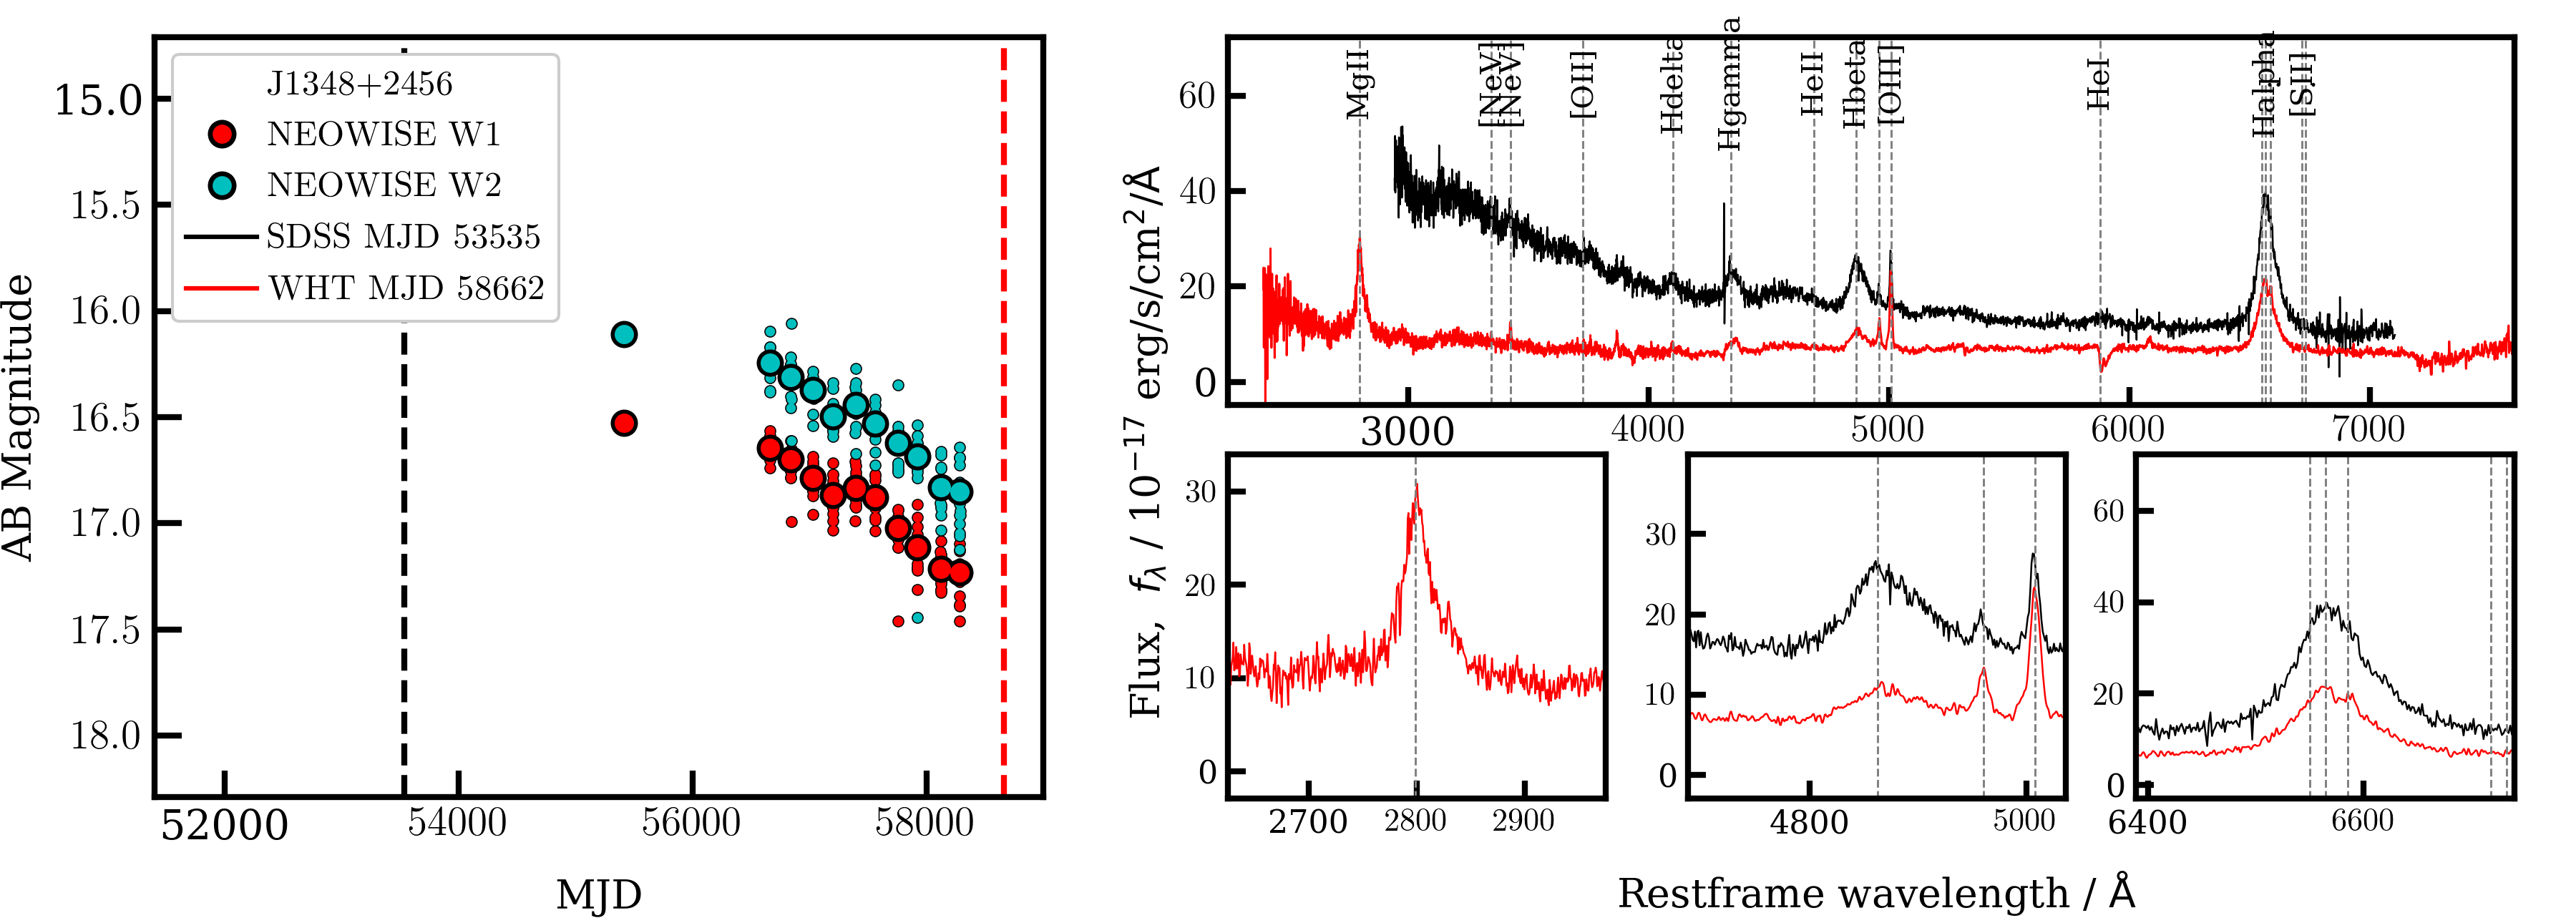
\includegraphics[width=16.7cm, trim=0.0cm 0.05cm 0.2cm 0.1cm, clip]
  {../plots/LCs_and_spectra/J1348+2456_landscape_temp.png}
  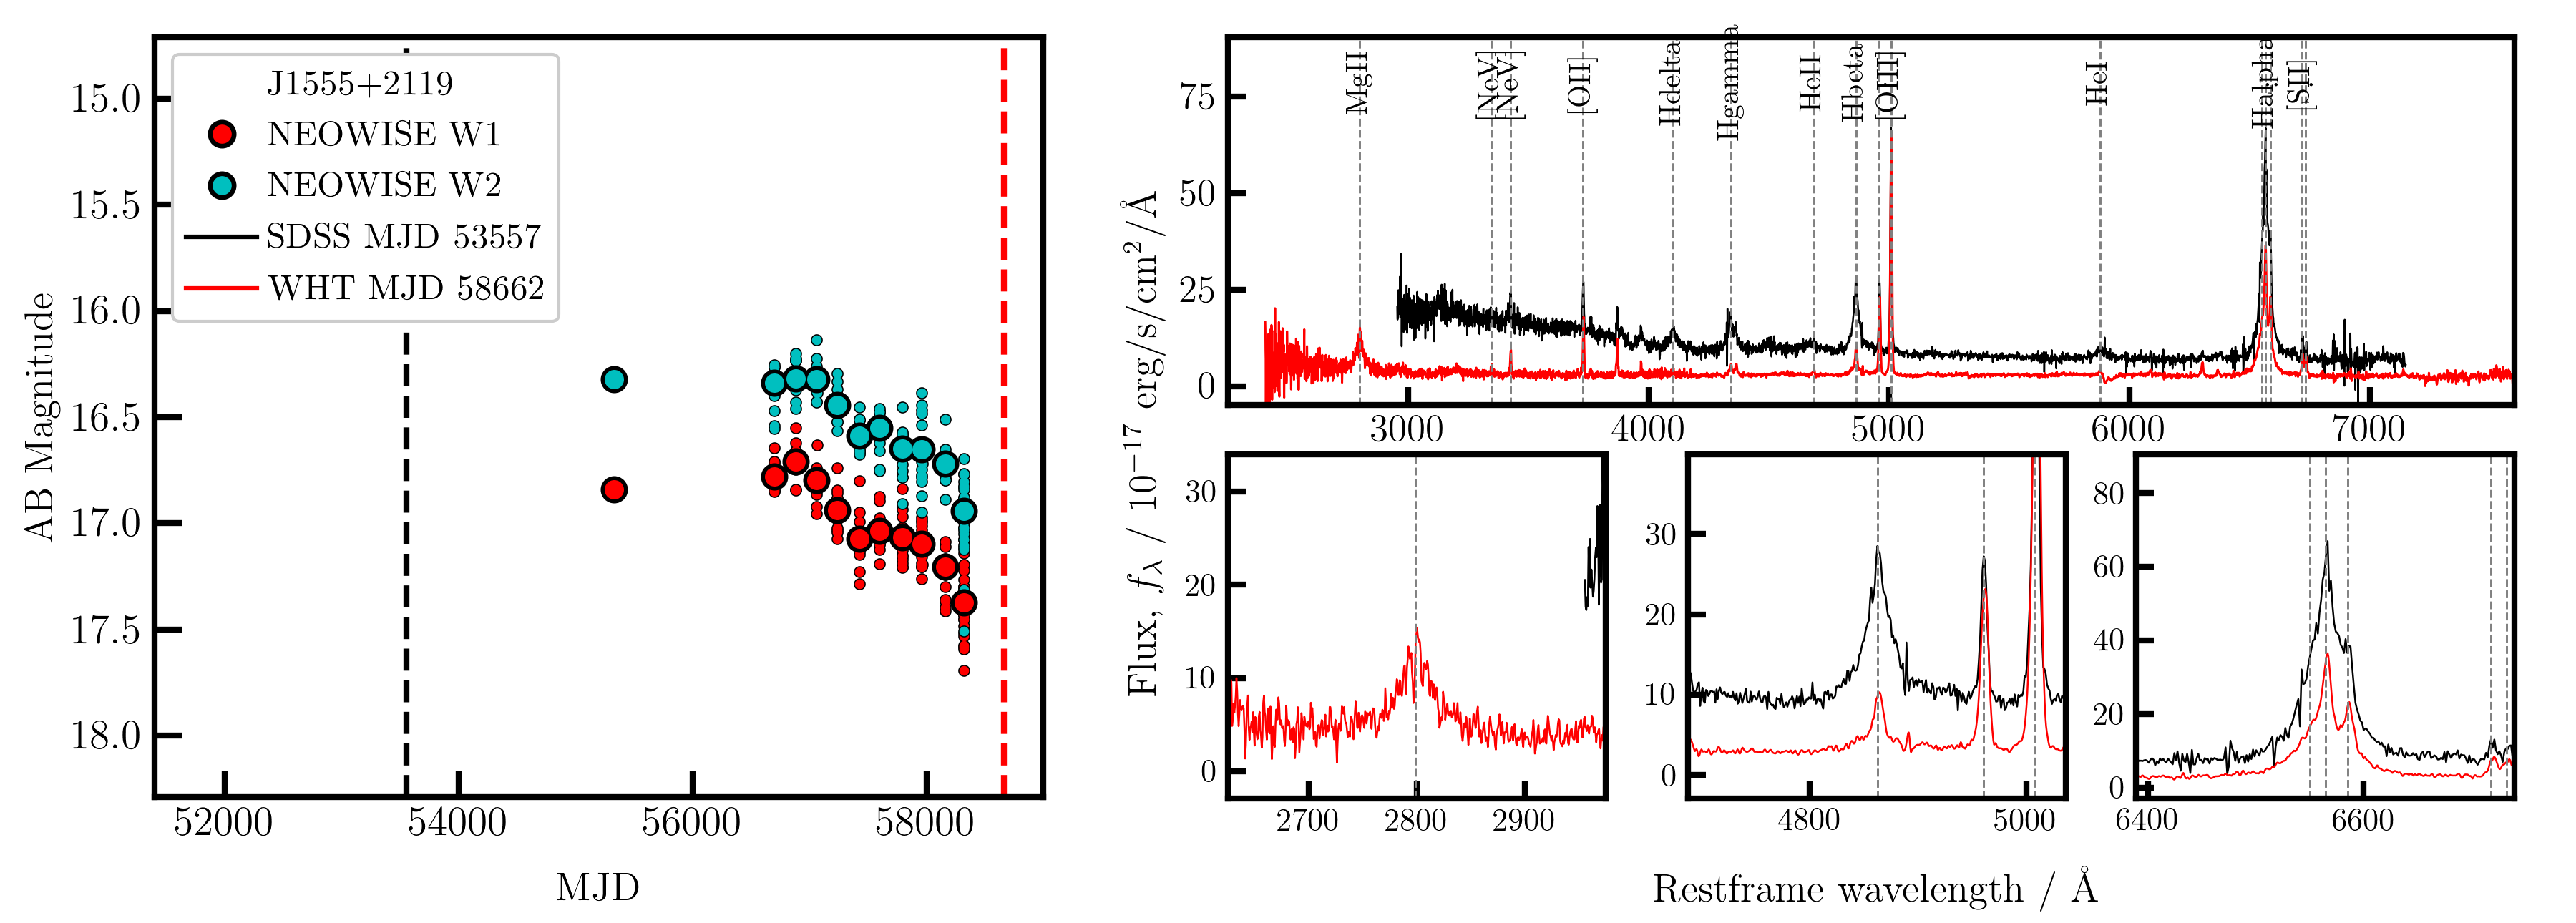
\includegraphics[width=16.7cm, trim=0.0cm 0.05cm 0.2cm 0.1cm, clip]
  {../plots/LCs_and_spectra/J1555+2119_landscape_temp.png}
  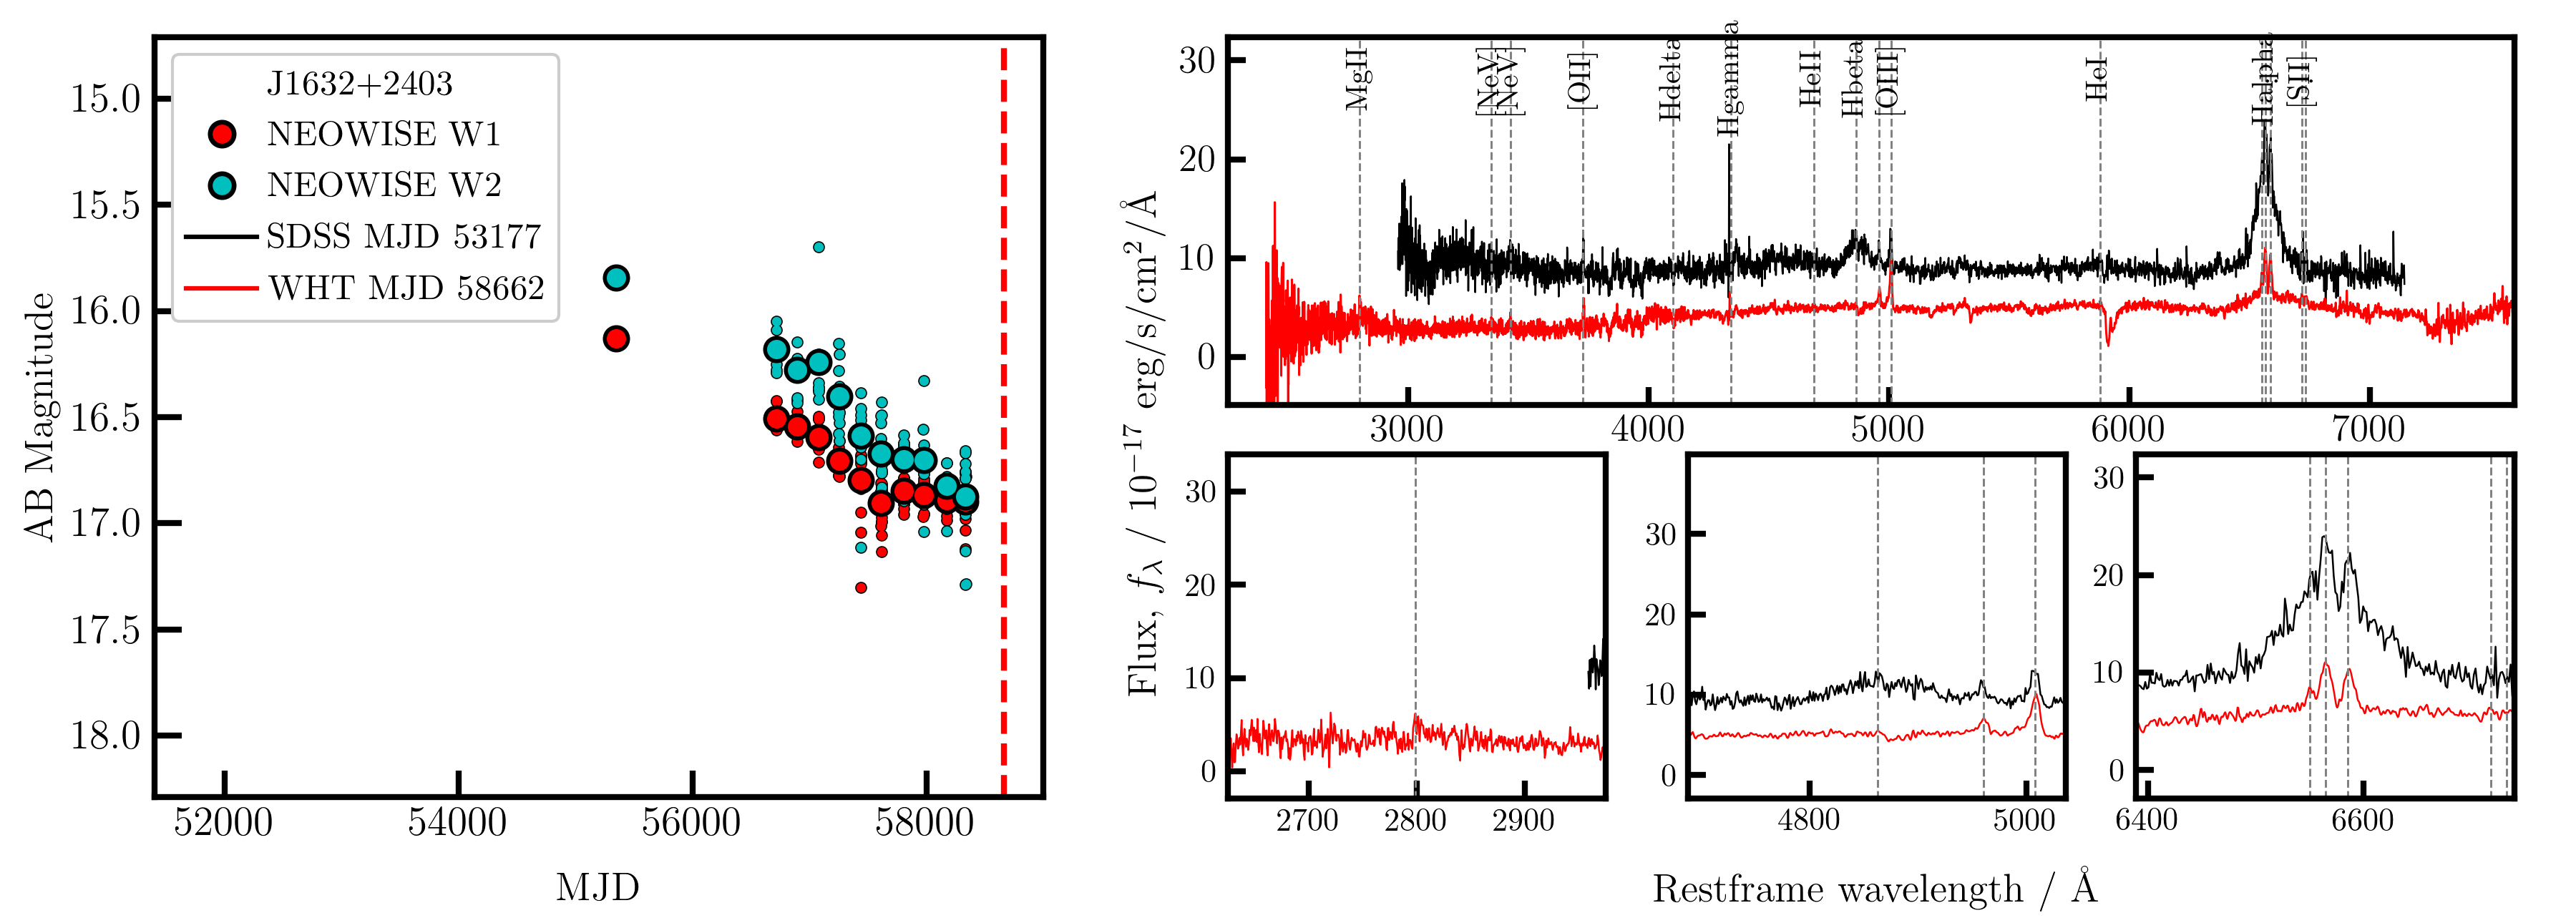
\includegraphics[width=16.7cm, trim=0.0cm 0.0cm  0.2cm 0.1cm, clip]
  {../plots/LCs_and_spectra/J1634+1118_landscape_temp.png}
  \vspace{-12pt}
  \caption[]{}
  \label{fig:faders}
\end{figure*}

%%   RISERS
 \begin{figure*}
  \centering
  %% trim=l b r t
  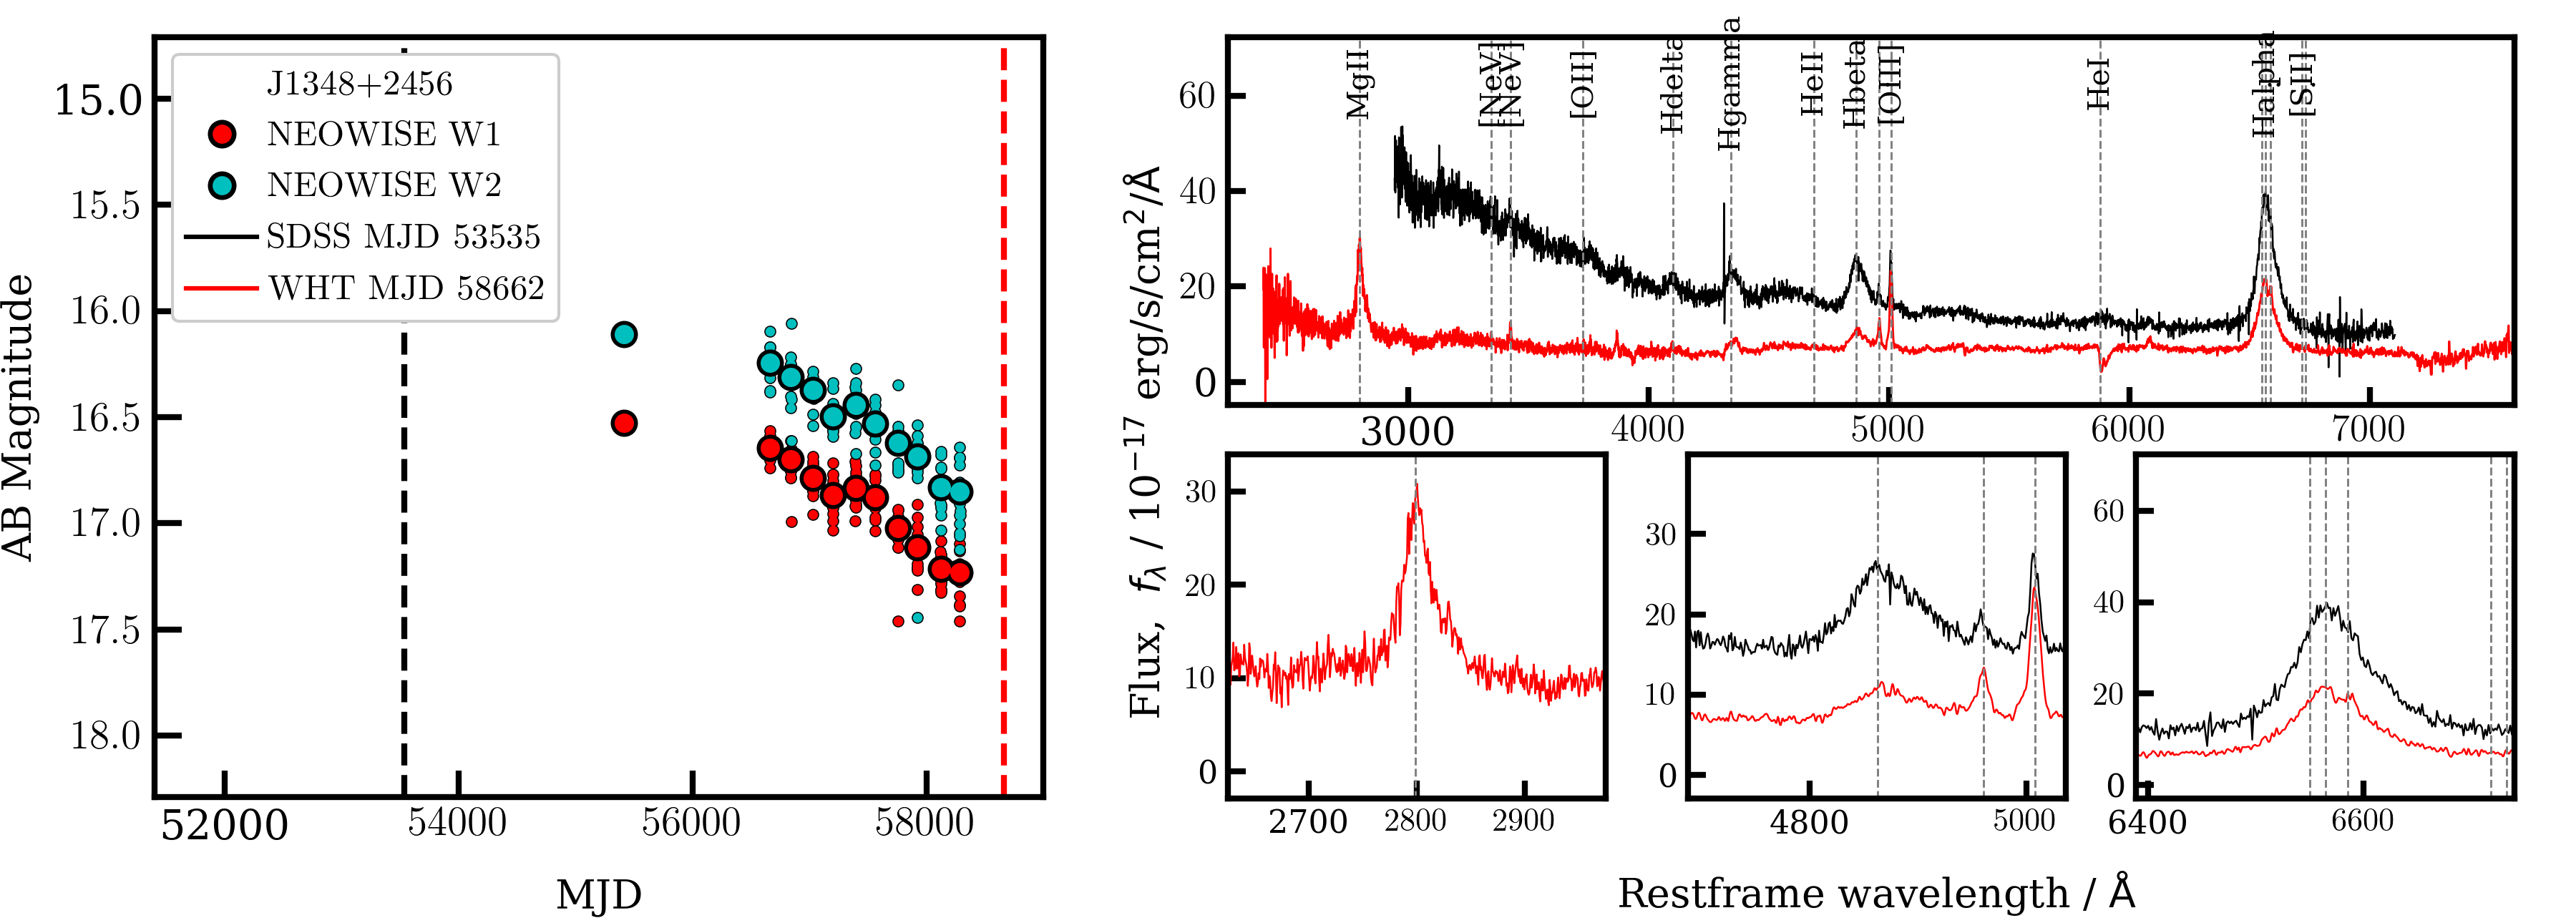
\includegraphics[width=16.7cm, trim=0.0cm 0.05cm 0.2cm 0.1cm, clip]
  {../plots/LCs_and_spectra/J1348+2456_landscape_temp.png}
  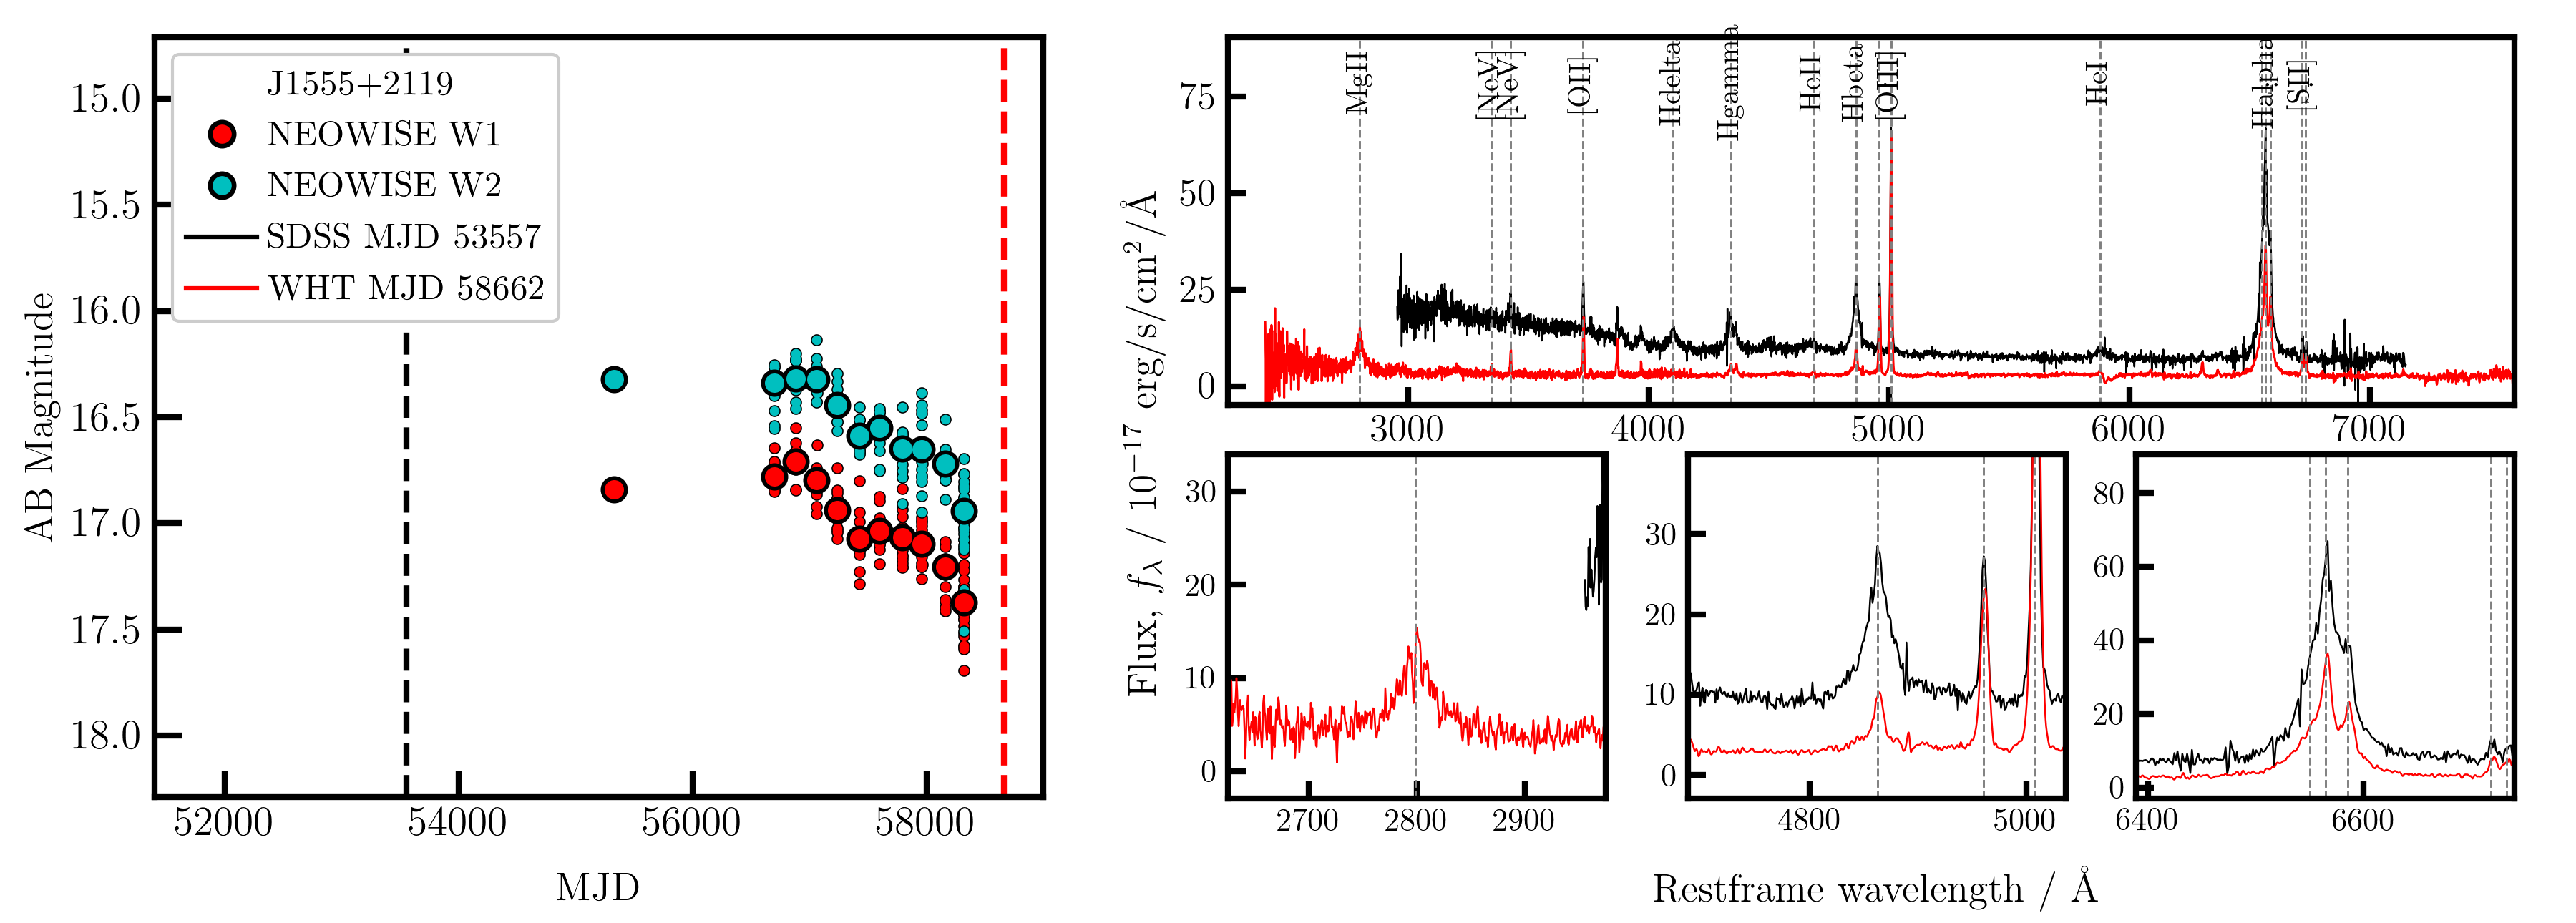
\includegraphics[width=16.7cm, trim=0.0cm 0.05cm 0.2cm 0.1cm, clip]
  {../plots/LCs_and_spectra/J1555+2119_landscape_temp.png}
  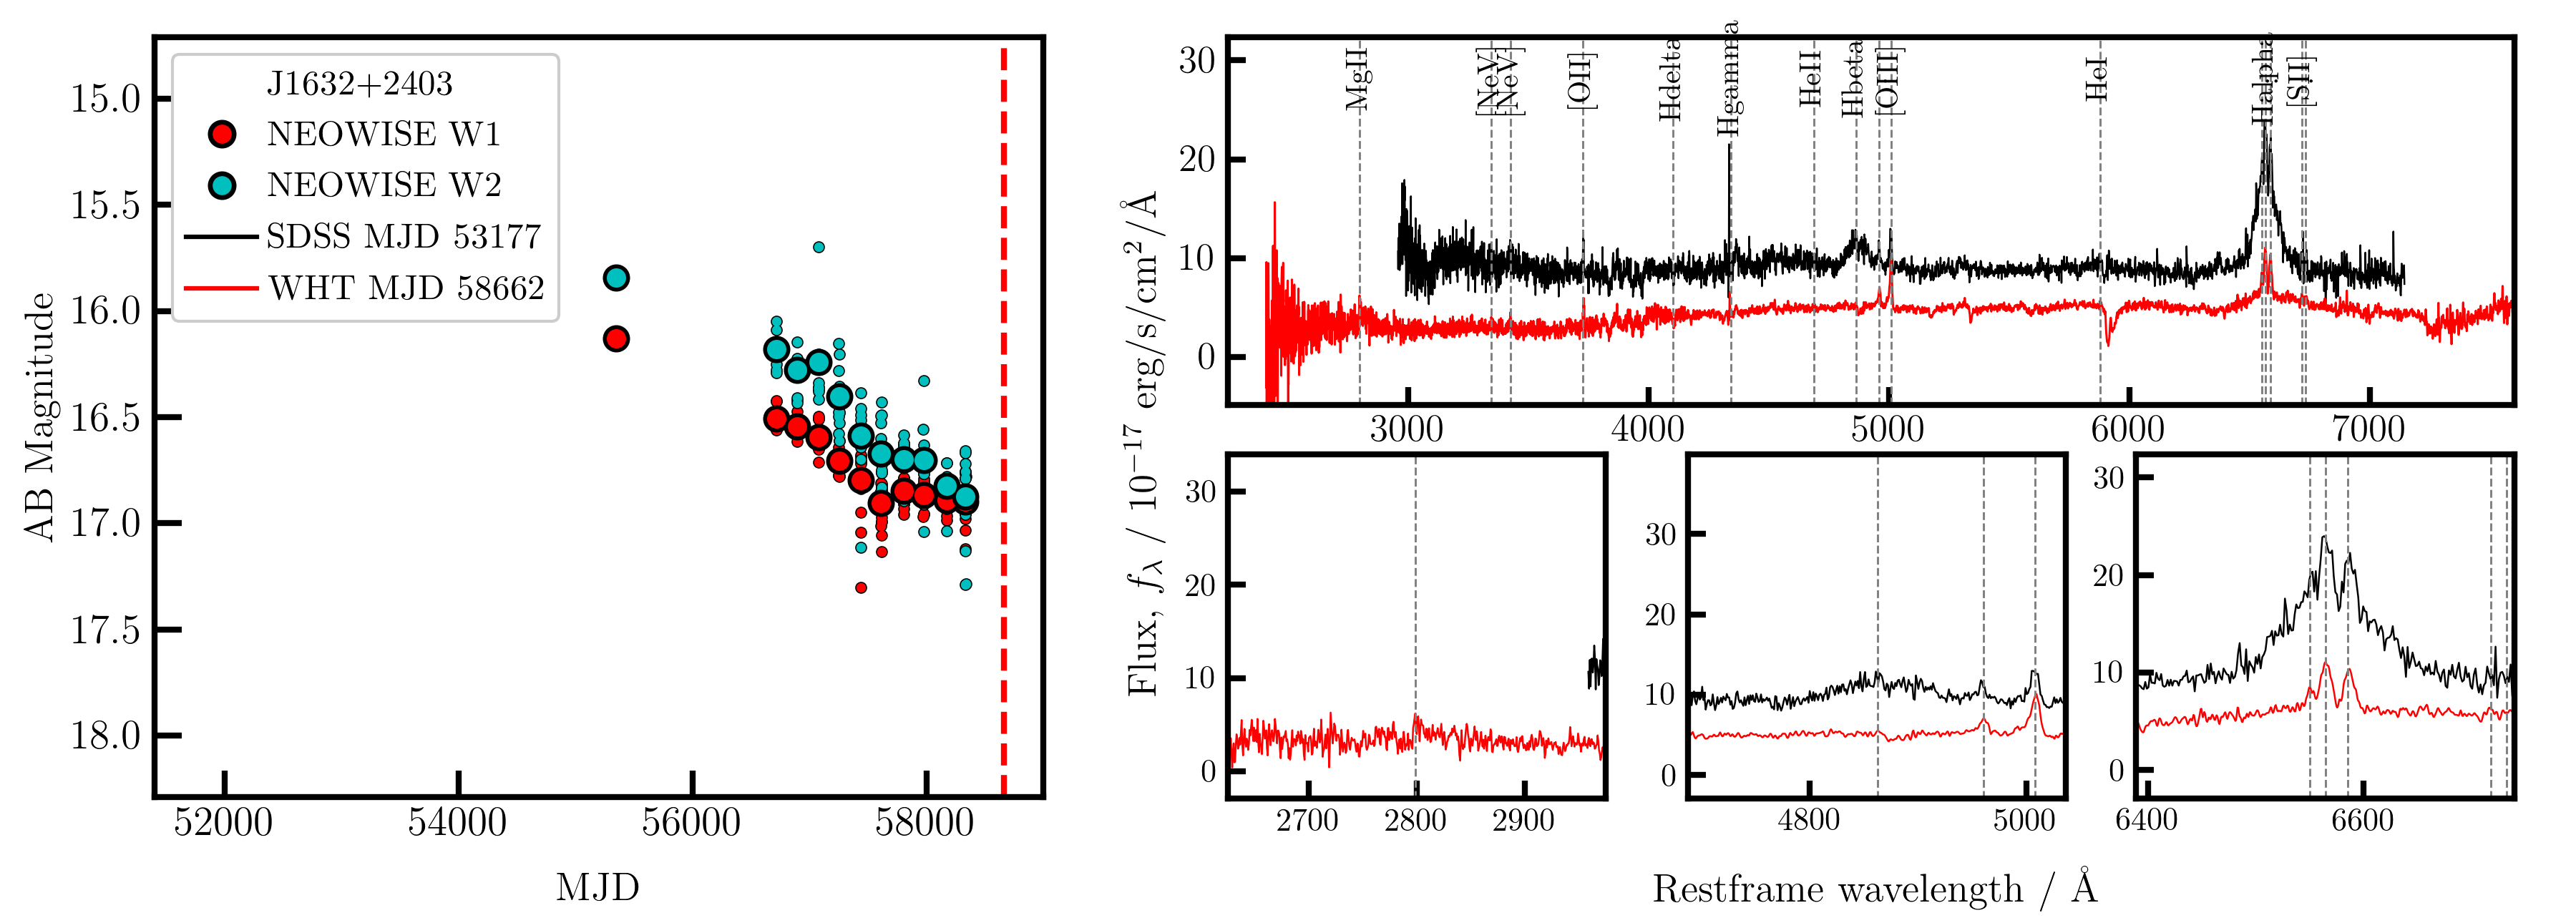
\includegraphics[width=16.7cm, trim=0.0cm 0.0cm  0.2cm 0.1cm, clip]
  {../plots/LCs_and_spectra/J1634+1118_landscape_temp.png}
  \vspace{-12pt}
  \caption[]{}
  \label{fig:risers}
\end{figure*}


\subsection{Maths}
\label{sec:maths} % used for referring to this section from elsewhere

Simple mathematics can be inserted into the flow of the text e.g. $2\times3=6$
or $v=220$\,km\,s$^{-1}$, but more complicated expressions should be entered
as a numbered equation:

\begin{equation}
    x=\frac{-b\pm\sqrt{b^2-4ac}}{2a}.
	\label{eq:quadratic}
\end{equation}

Refer back to them as e.g. equation~(\ref{eq:quadratic}).

\subsection{Figures and tables}

Figures and tables should be placed at logical positions in the text. Don't
worry about the exact layout, which will be handled by the publishers.

Figures are referred to as e.g. Fig.~\ref{fig:example_figure}, and tables as
e.g. Table~\ref{tab:example_table}.

% Example figure
\begin{figure}
	% To include a figure from a file named example.*
	% Allowable file formats are eps or ps if compiling using latex
	% or pdf, png, jpg if compiling using pdflatex
	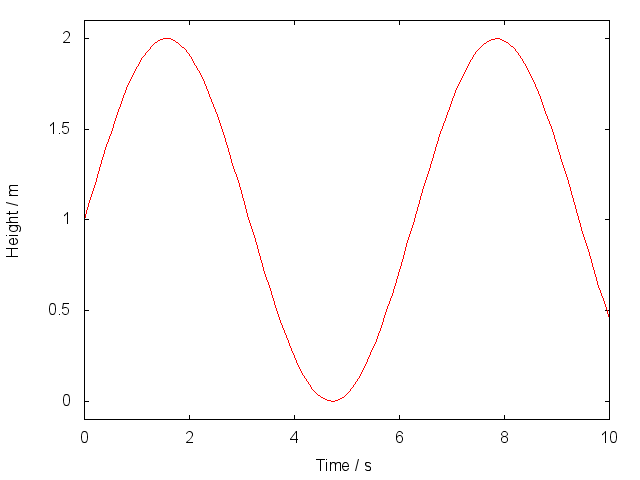
\includegraphics[width=\columnwidth]{example}
    \caption{This is an example figure. Captions appear below each figure.
	Give enough detail for the reader to understand what they're looking at,
	but leave detailed discussion to the main body of the text.}
    \label{fig:example_figure}
\end{figure}

% Example table
\begin{table}
	\centering
	\caption{This is an example table. Captions appear above each table.
	Remember to define the quantities, symbols and units used.}
	\label{tab:example_table}
	\begin{tabular}{lccr} % four columns, alignment for each
		\hline
		A & B & C & D\\
		\hline
		1 & 2 & 3 & 4\\
		2 & 4 & 6 & 8\\
		3 & 5 & 7 & 9\\
		\hline
	\end{tabular}
\end{table}

\subsection{Disk Emitters} 
cf. our objects with e.g. Figure 11 \citet{Shen2011} and J161742.53+322234.3. 
Are any of the WHT CLQs Shen ``Disk Emitters''  
(``bit \# 1 set = disk emitter candidates;'')


\section{Discussion}\label{sec:discussion} 
Lorem ipsum dolor sit amet, consectetur adipiscing elit. Aliquam porta sodales est, vel cursus risus porta non. Vivamus vel pretium velit. Sed fringilla suscipit felis, nec iaculis lacus convallis ac. Fusce pellentesque condimentum dolor, quis vehicula tortor hendrerit sed. Class aptent taciti sociosqu ad litora torquent per conubia nostra, per inceptos himenaeos. Etiam interdum tristique diam eu blandit. Donec in lacinia libero.

Sed elit massa, eleifend non sodales a, commodo ut felis. Sed id pretium felis. Vestibulum et turpis vitae quam aliquam convallis. Sed id ligula eu nulla ultrices tempus. Phasellus mattis erat quis metus dignissim malesuada. Nulla tincidunt quam volutpat nibh facilisis euismod. Cras vel auctor neque. Nam quis diam risus.

Nunc semper quam et leo interdum vulputate eu quis magna. Sed nec arcu at orci egestas convallis. Aenean quam velit, aliquam vitae viverra in, elementum vel elit. Nunc suscipit aliquet sapien a suscipit. Cras nulla ipsum, posuere eu fringilla sit amet, dapibus ultricies nulla. Nullam eu augue id purus mollis dignissim sed et libero. Phasellus eget justo sed neque pellentesque egestas nec id arcu. Donec facilisis pulvinar sapien et fringilla. Suspendisse vestibulum rhoncus sapien id laoreet. Morbi et orci vitae tortor imperdiet imperdiet. In hac habitasse platea dictumst. Vivamus vel neque id mi ultrices tristique. Integer quam libero, ornare vel gravida in, feugiat a ante. Nam dapibus, tellus vitae pellentesque cursus, dui nisl egestas augue, non fermentum nisl est nec nisi. Vestibulum nec mi justo, eget dapibus velit.

Cras in laoreet mauris. Vivamus nec nulla a dui commodo adipiscing. Proin vulputate lectus nec arcu iaculis sit amet auctor ligula ultricies. Phasellus condimentum gravida tincidunt. Phasellus et mauris ac nibh vestibulum vehicula. Morbi et augue id purus gravida sagittis quis in sem. Phasellus quis risus bibendum eros luctus auctor.

Etiam mollis viverra nisi eget aliquet. Aliquam erat volutpat. Vivamus tristique, nisl eu malesuada semper, libero tortor convallis elit, a scelerisque orci nisi lacinia turpis. In lacinia ultrices volutpat. Proin ultrices luctus tellus, in placerat eros tincidunt id. Ut varius iaculis quam in consequat. Nulla nec orci est, sit amet pellentesque nisl. Mauris non cursus lectus. Praesent placerat leo vel erat gravida lacinia. Donec vehicula consectetur lectus vitae luctus. Praesent nisl justo, laoreet elementum facilisis vel, tristique ac enim. Etiam vel quam ut quam eleifend tincidunt. Suspendisse sit amet eros vel elit ullamcorper laoreet. Etiam venenatis sodales turpis, nec lacinia ligula hendrerit nec. Nam eu vulputate purus. Quisque facilisis congue metus, sed imperdiet lorem rhoncus sit amet.


\section{Conclusions}\label{sec:conclusions} 
Donec elit tortor, scelerisque ac molestie id, hendrerit sit amet ipsum. Maecenas non tempus sem. Pellentesque ut enim velit, eu sagittis elit. Nulla in elementum erat. In dictum arcu at nisi porttitor commodo. Donec felis felis, elementum sit amet ultrices ac, interdum nec ante. Nullam eget faucibus lectus. Donec vitae eros sapien, et faucibus ligula. Aenean pharetra viverra fermentum.

The last numbered section should briefly summarise what has been done, and describe
the final conclusions which the authors draw from their work.

\begin{itemize}
  \item Sed sed ipsum diam. In risus tortor, sagittis eu auctor in, varius in dui. Mauris a nunc ut ligula ullamcorper tincidunt. 
  \item Nunc aliquam eros ac risus pellentesque aliquam. Phasellus augue velit, varius at porttitor sit amet, pretium eget felis. 
  \item Ut mollis tellus elementum magna porttitor rutrum. Etiam blandit leo eget est consectetur imperdiet. 
 \item Quisque et diam nec orci vulputate varius vitae id sapien.
\end{itemize}



\section*{Acknowledgements}

The Acknowledgements section is not numbered. Here you can thank helpful
colleagues, acknowledge funding agencies, telescopes and facilities used etc.
Try to keep it short.

%%%%%%%%%%%%%%%%%%%%%%%%%%%%%%%%%%%%%%%%%%%%%%%%%%

%%%%%%%%%%%%%%%%%%%% REFERENCES %%%%%%%%%%%%%%%%%%

% The best way to enter references is to use BibTeX:
\bibliographystyle{mnras}
\bibliography{/cos_pc19a_npr/programs/quasars/CIV_CLQs/tex/tester_mnras}




%%%         A P P E N D I C E S     %%%

\appendix

\section{Some extra material}
If you want to present additional material which would interrupt the
flow of the main paper, it can be placed in an Appendix which appears
after the list of references.

%% 
\begin{figure*}
  \centering
  %% trim=l b r t
  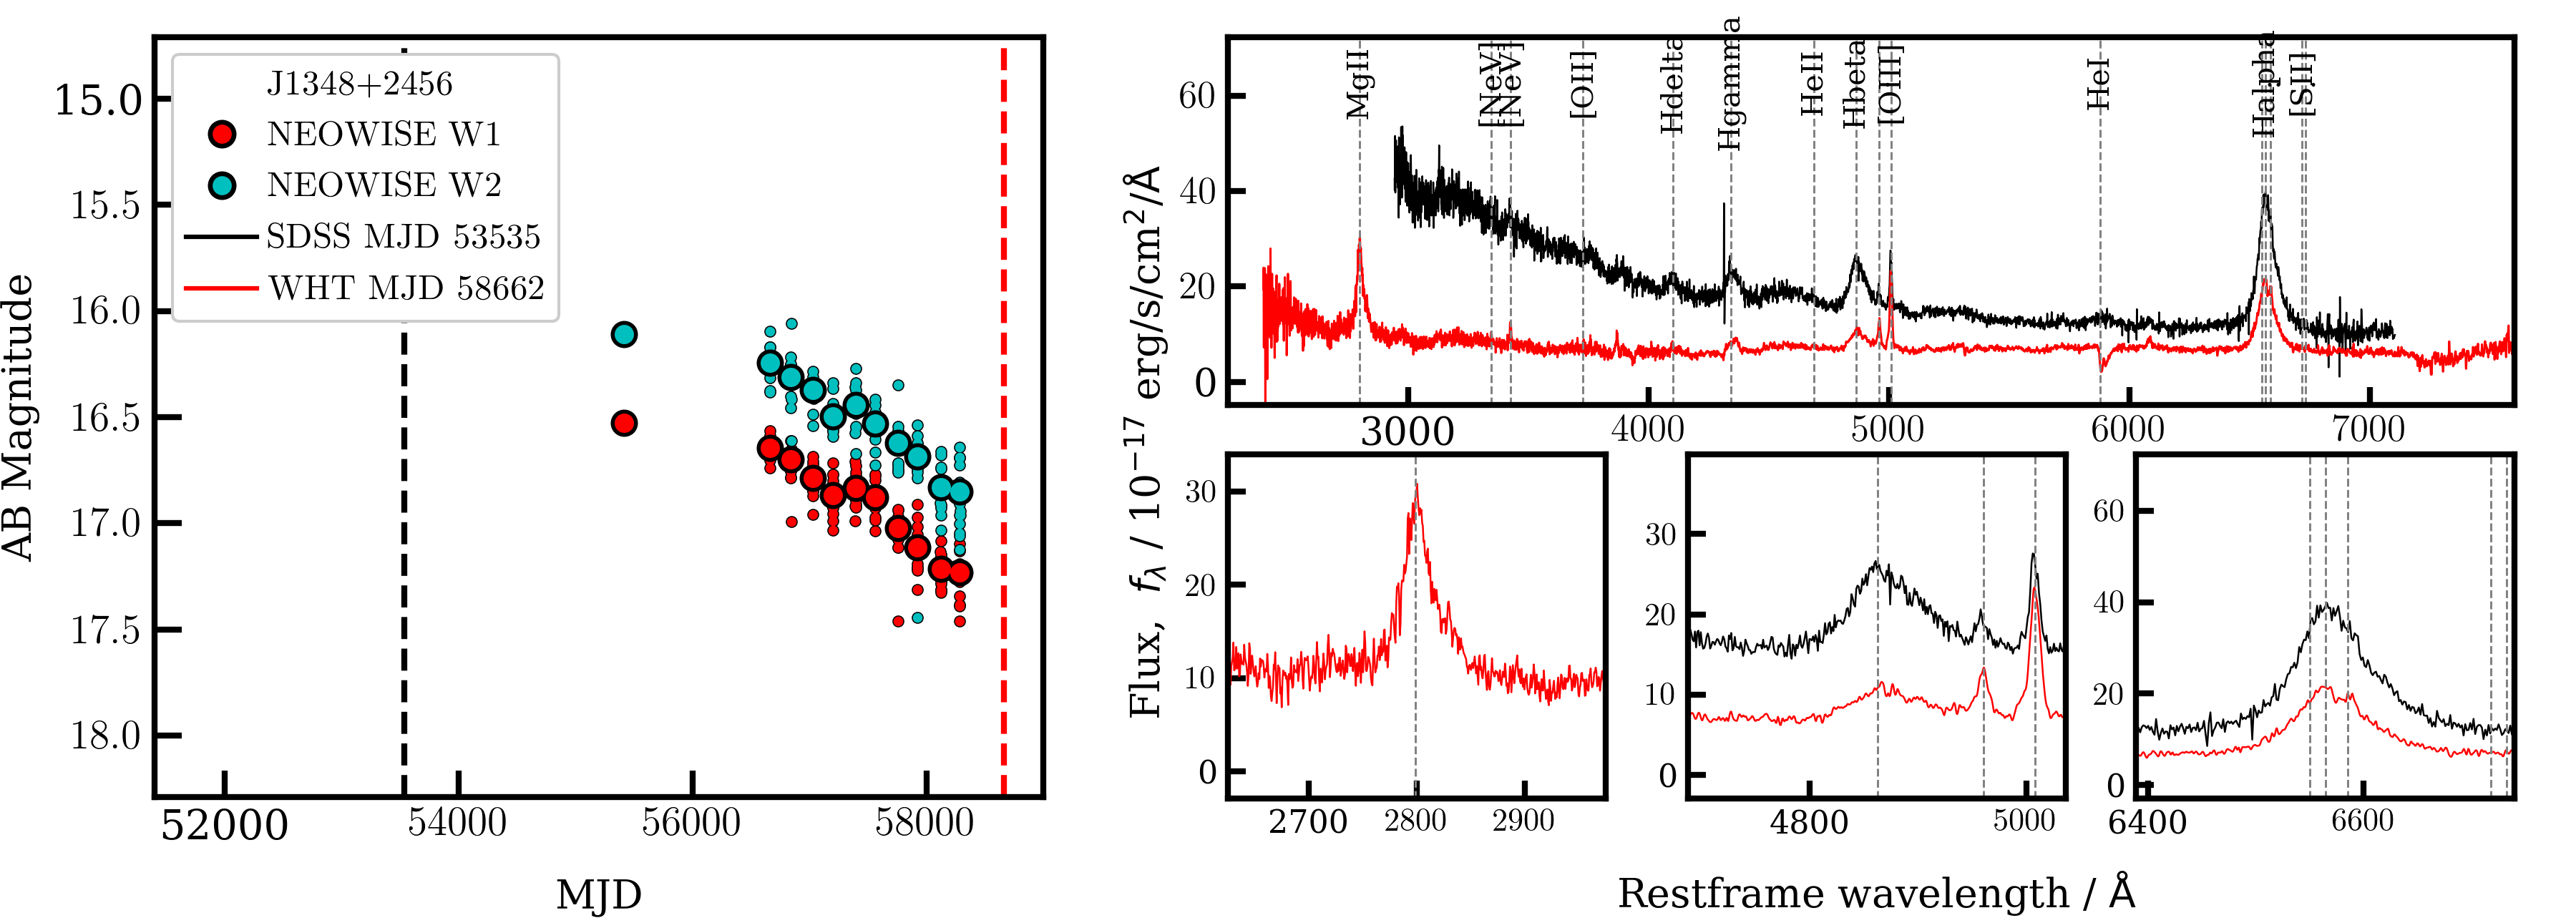
\includegraphics[width=16.7cm, trim=0.0cm 0.05cm 0.2cm 0.1cm, clip]
  {../plots/LCs_and_spectra/J1348+2456_landscape_temp.png}
  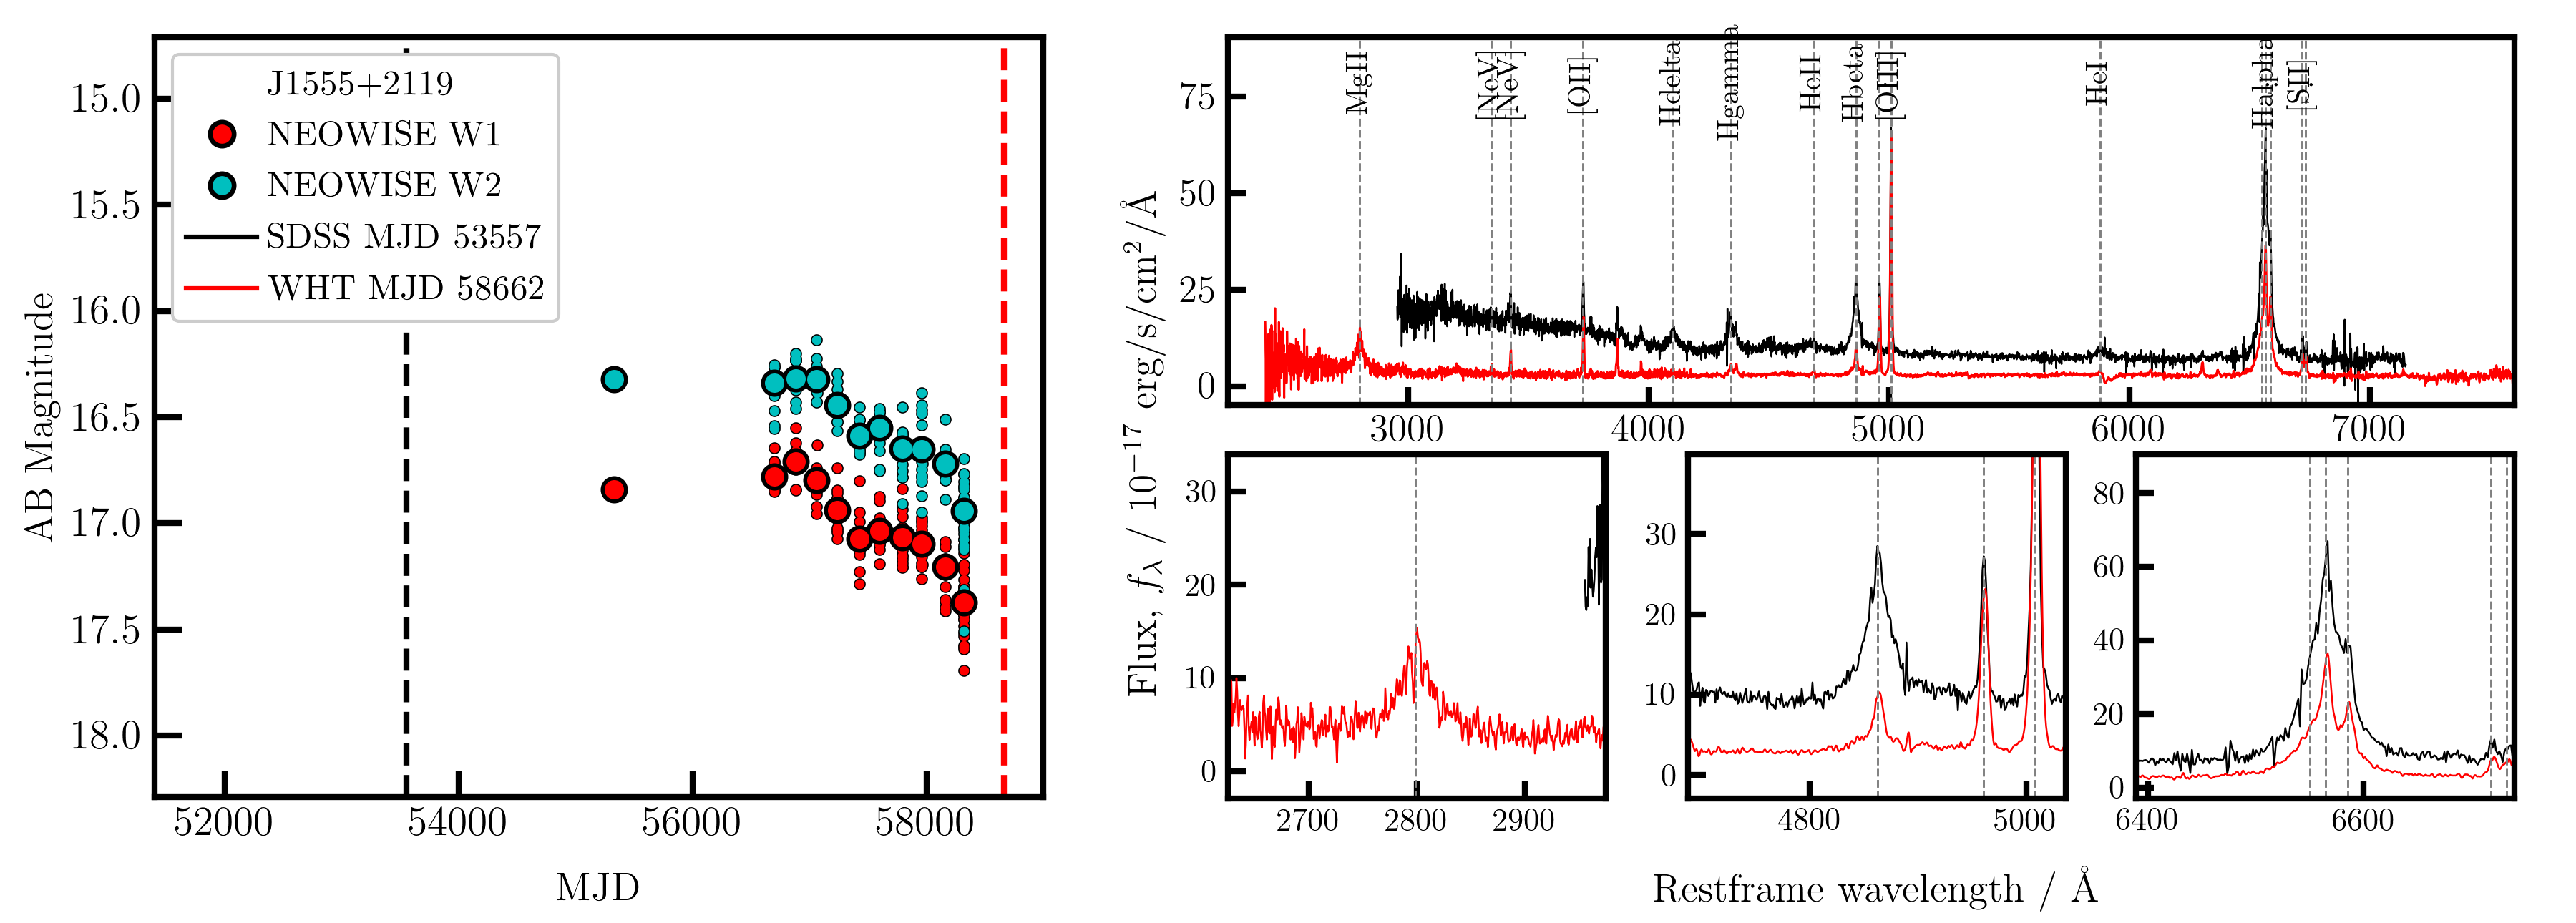
\includegraphics[width=16.7cm, trim=0.0cm 0.05cm 0.2cm 0.1cm, clip]
  {../plots/LCs_and_spectra/J1555+2119_landscape_temp.png}
  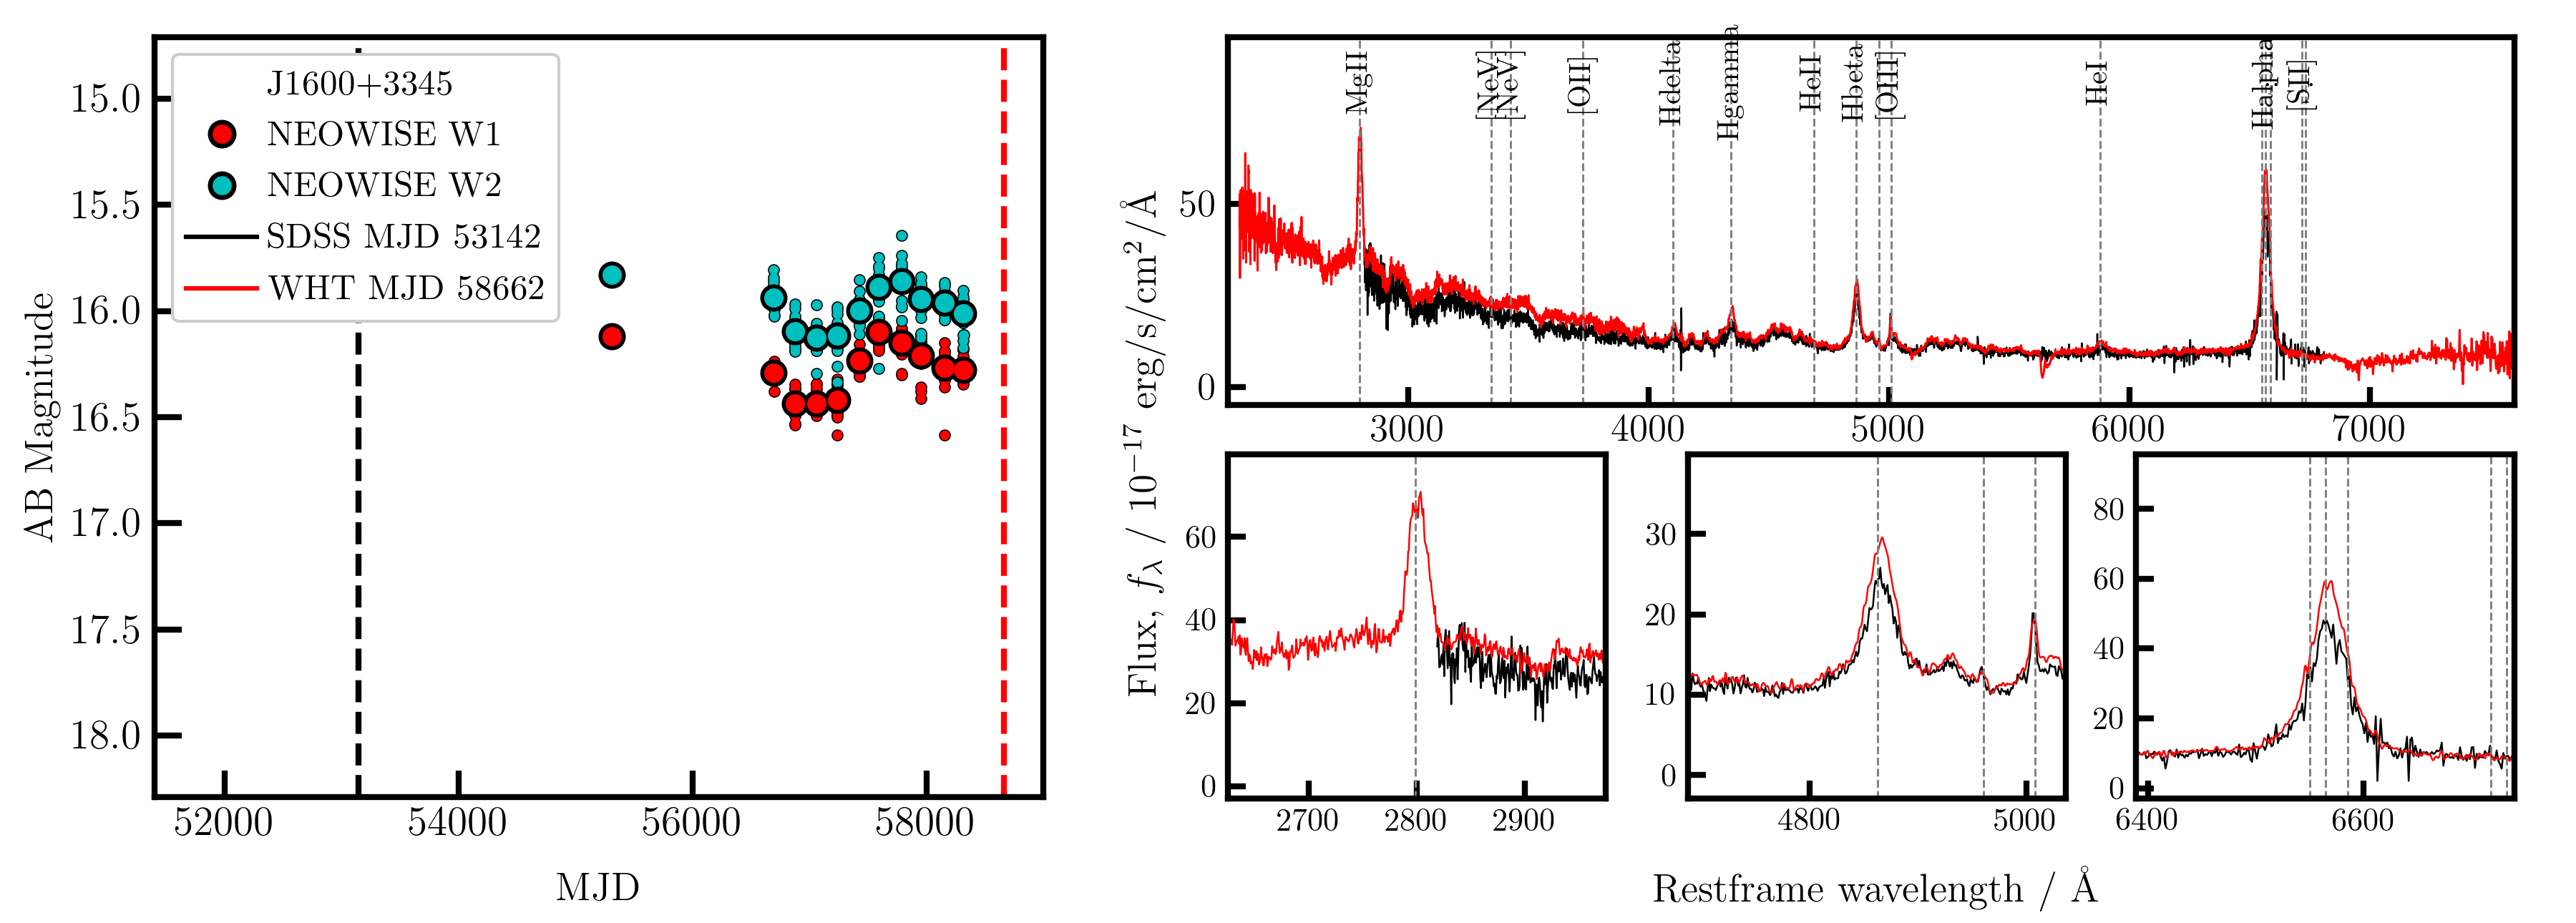
\includegraphics[width=16.7cm, trim=0.0cm 0.0cm  0.2cm 0.1cm, clip]
  {../plots/LCs_and_spectra/J1600+3345_landscape_temp.png}
  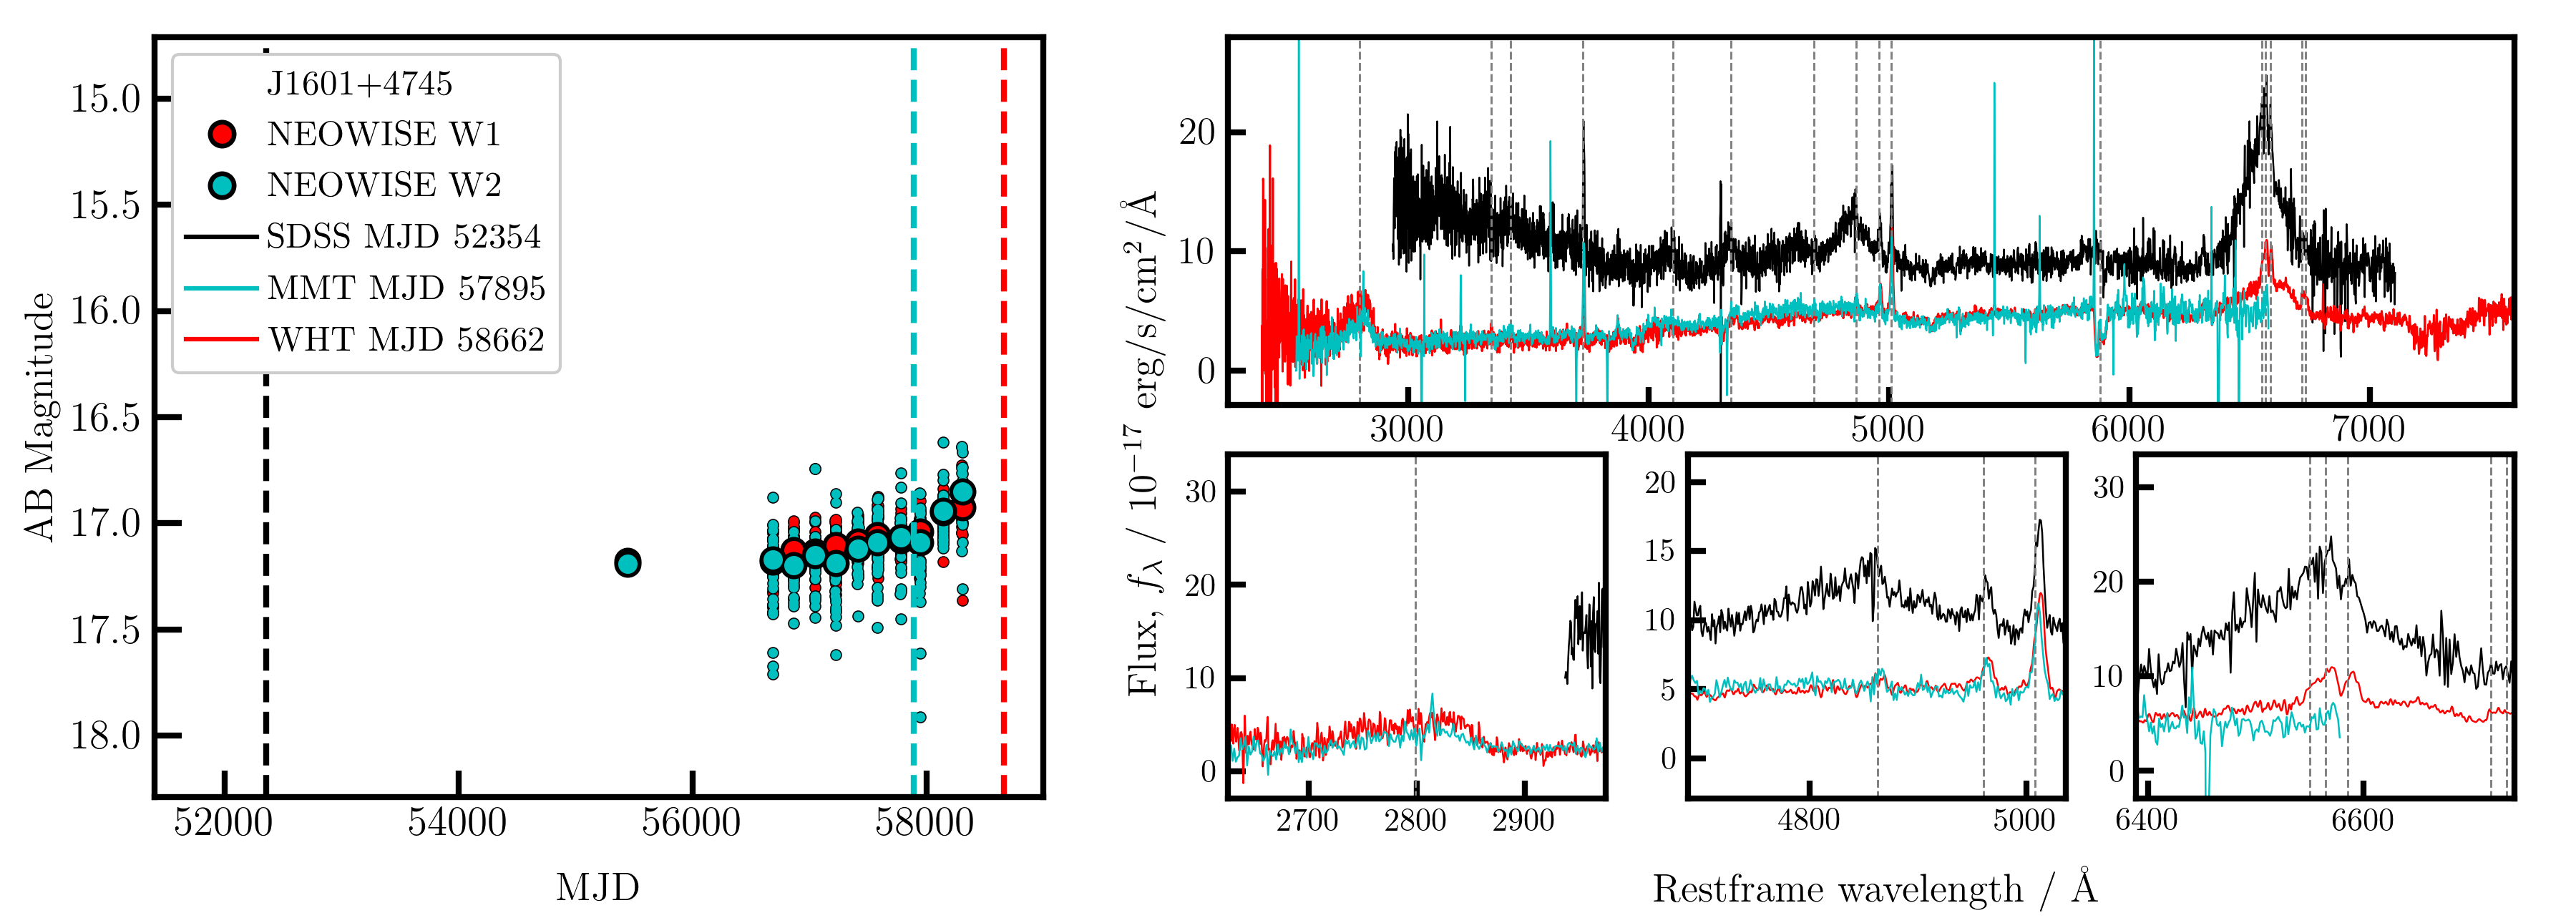
\includegraphics[width=16.7cm, trim=0.0cm 0.05cm 0.2cm 0.1cm, clip]
  {../plots/LCs_and_spectra/J1601+4745_landscape_temp.png}
  \vspace{-12pt}
  \caption[]{}
  \label{fig:all_spectra_a}
\end{figure*}

\begin{figure*}
  \centering
  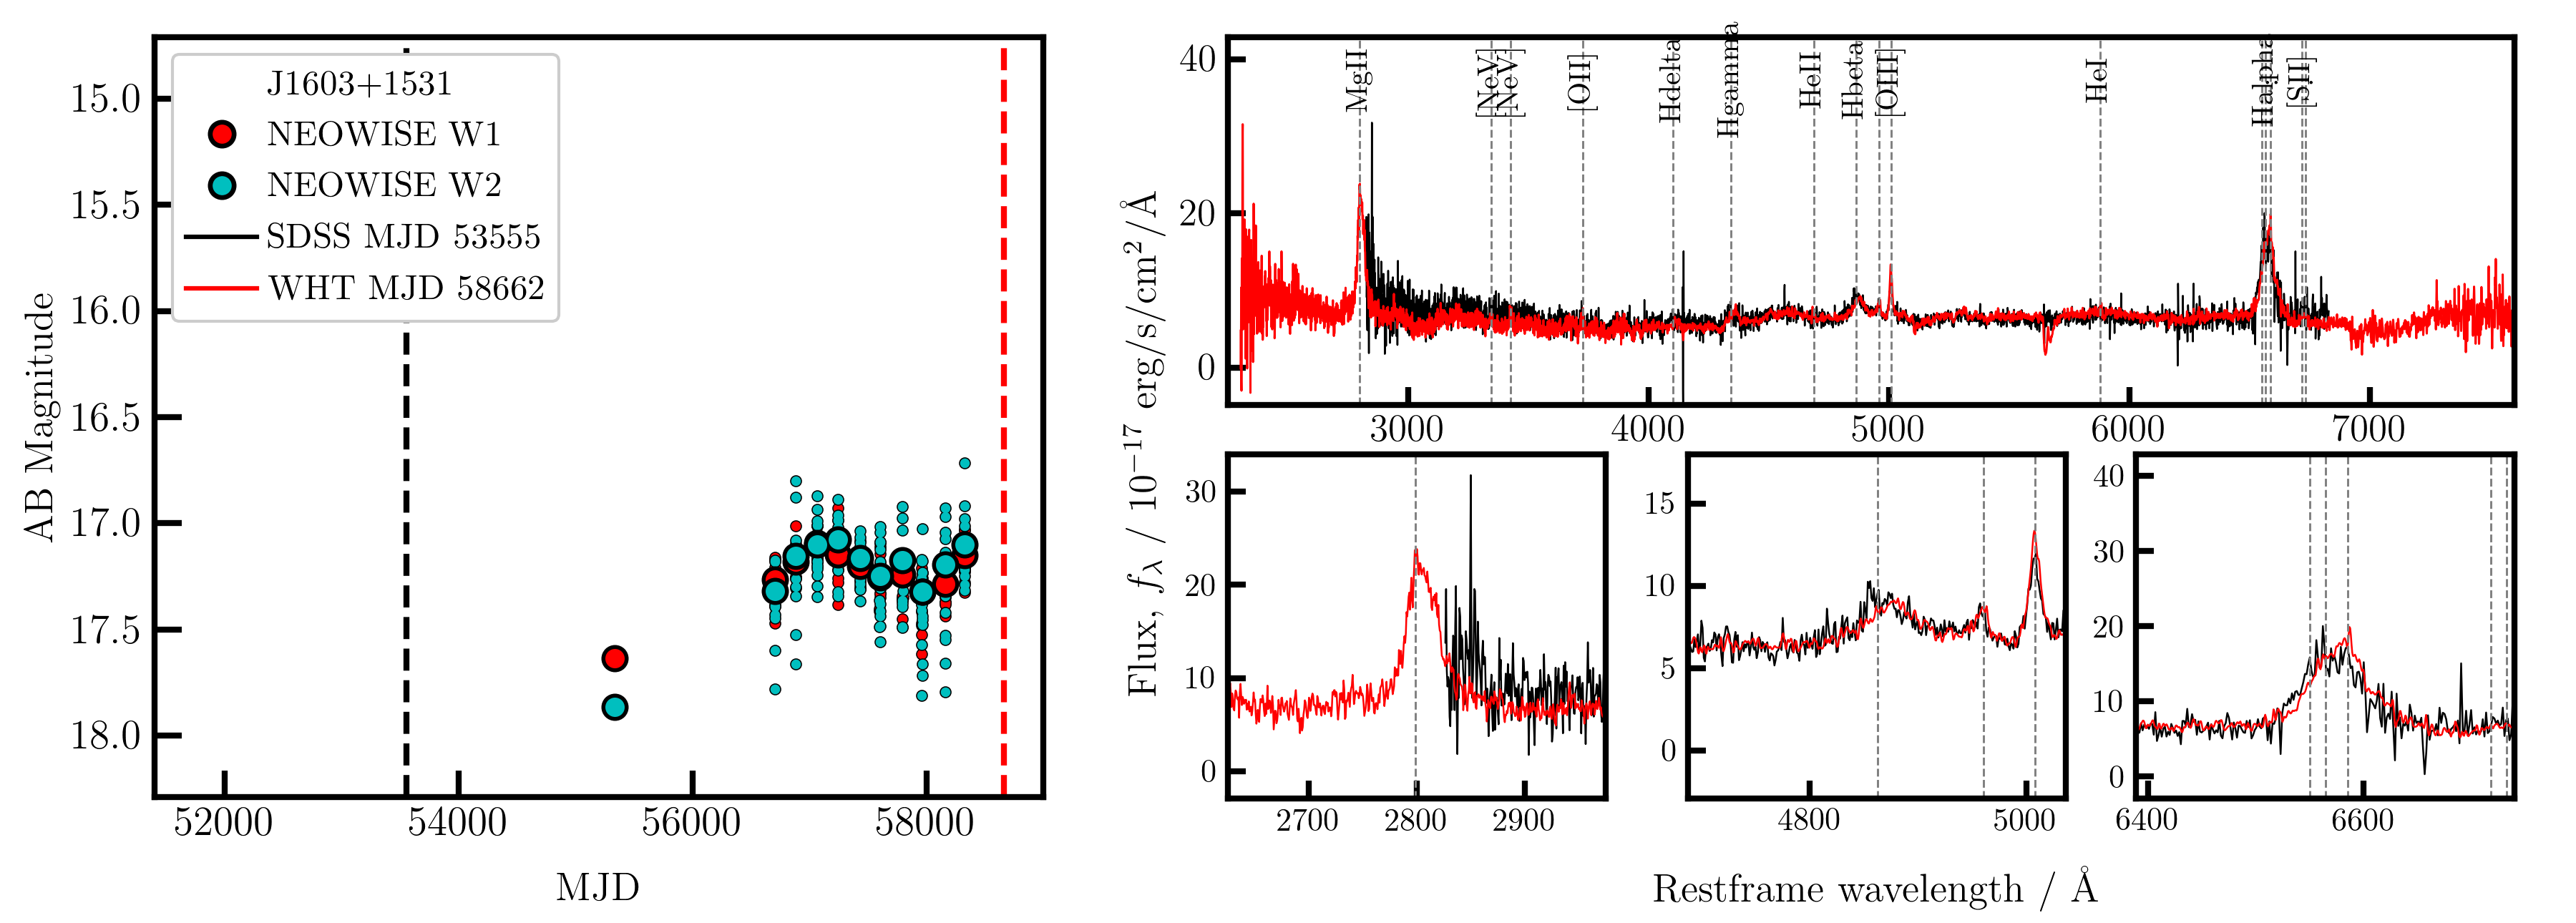
\includegraphics[width=16.7cm, trim=0.0cm 0.05cm 0.2cm 0.1cm, clip]
  {../plots/LCs_and_spectra/J1603+1531_landscape_temp.png}  
  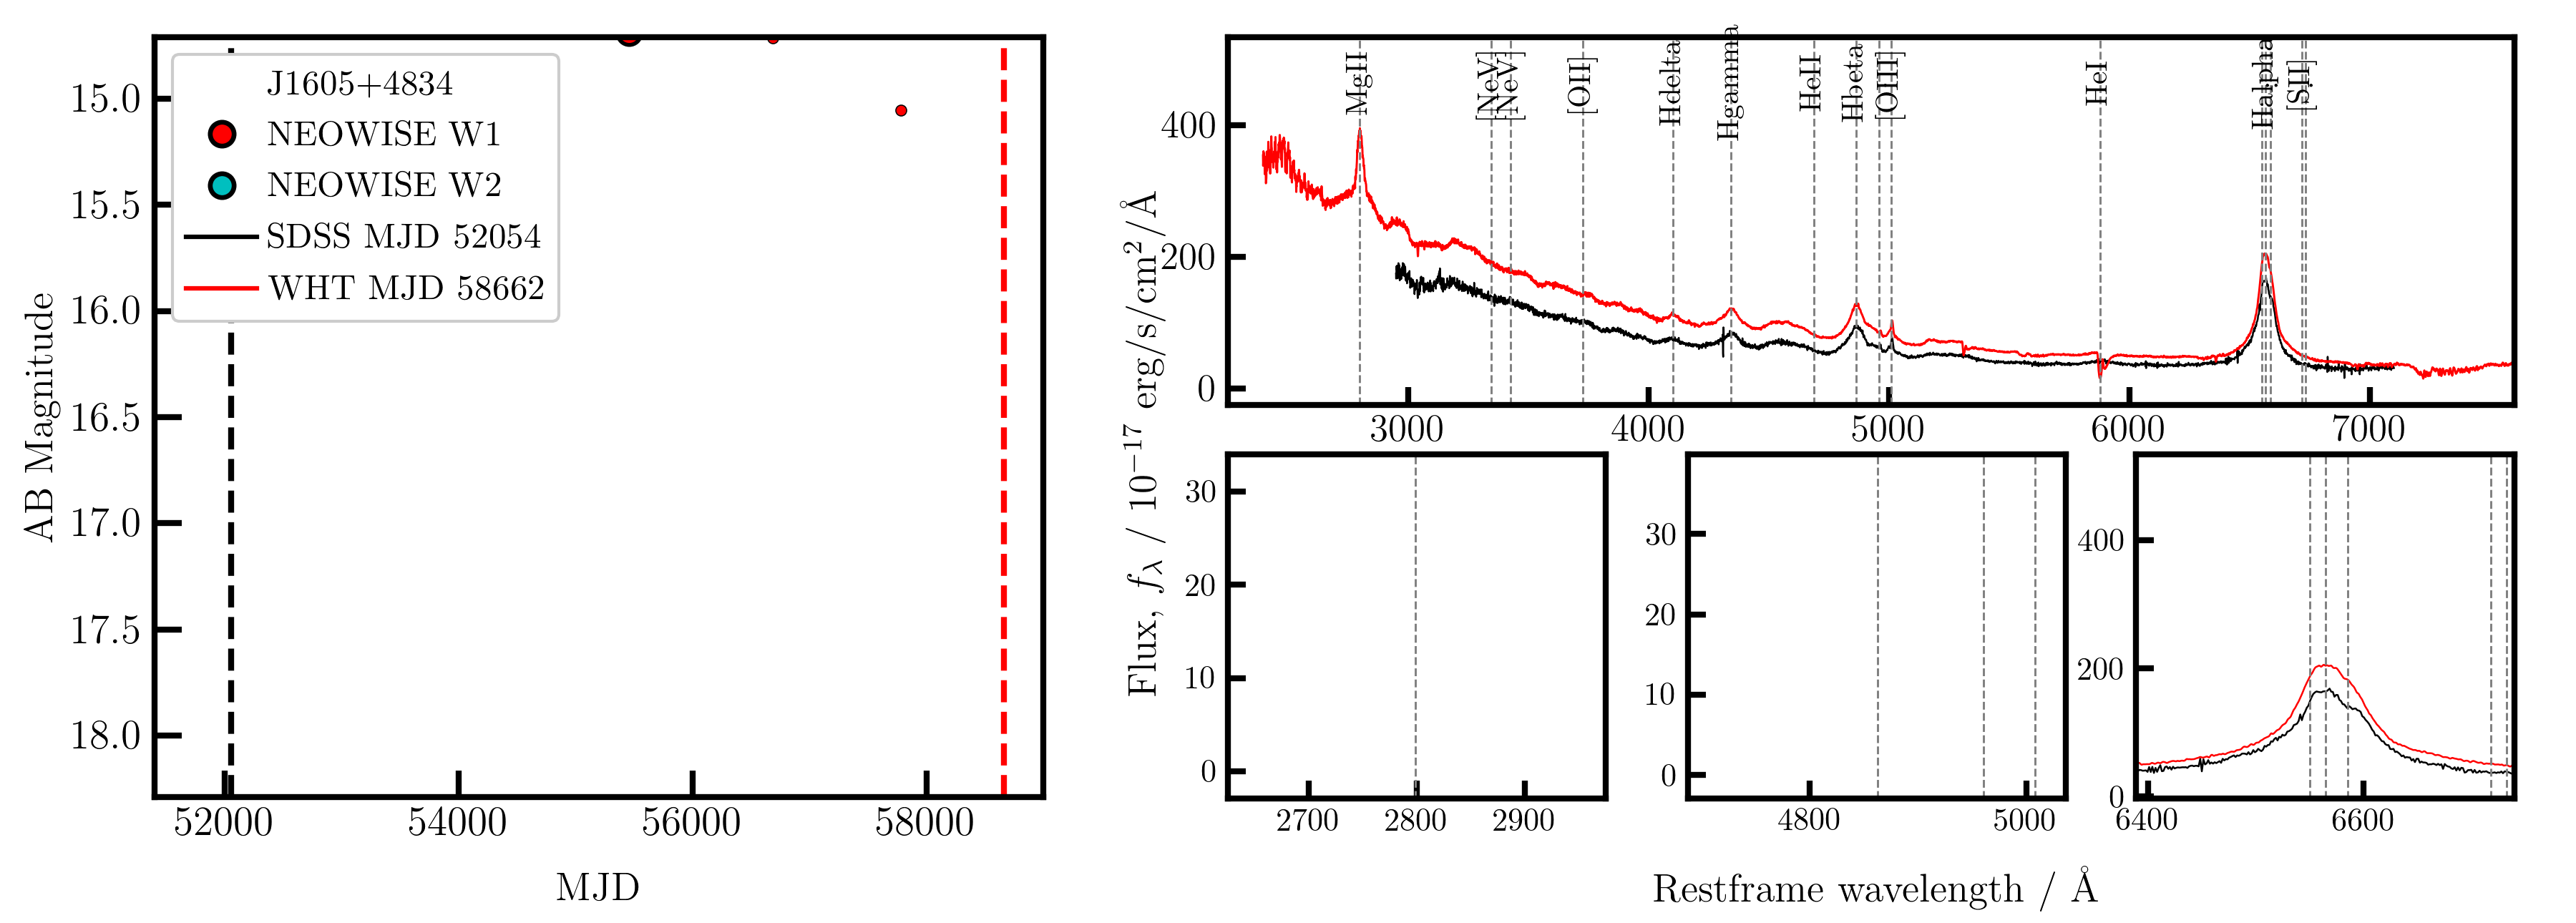
\includegraphics[width=16.7cm, trim=0.0cm 0.05cm 0.2cm 0.1cm, clip]
  {../plots/LCs_and_spectra/J1605+4834_landscape_temp.png}
  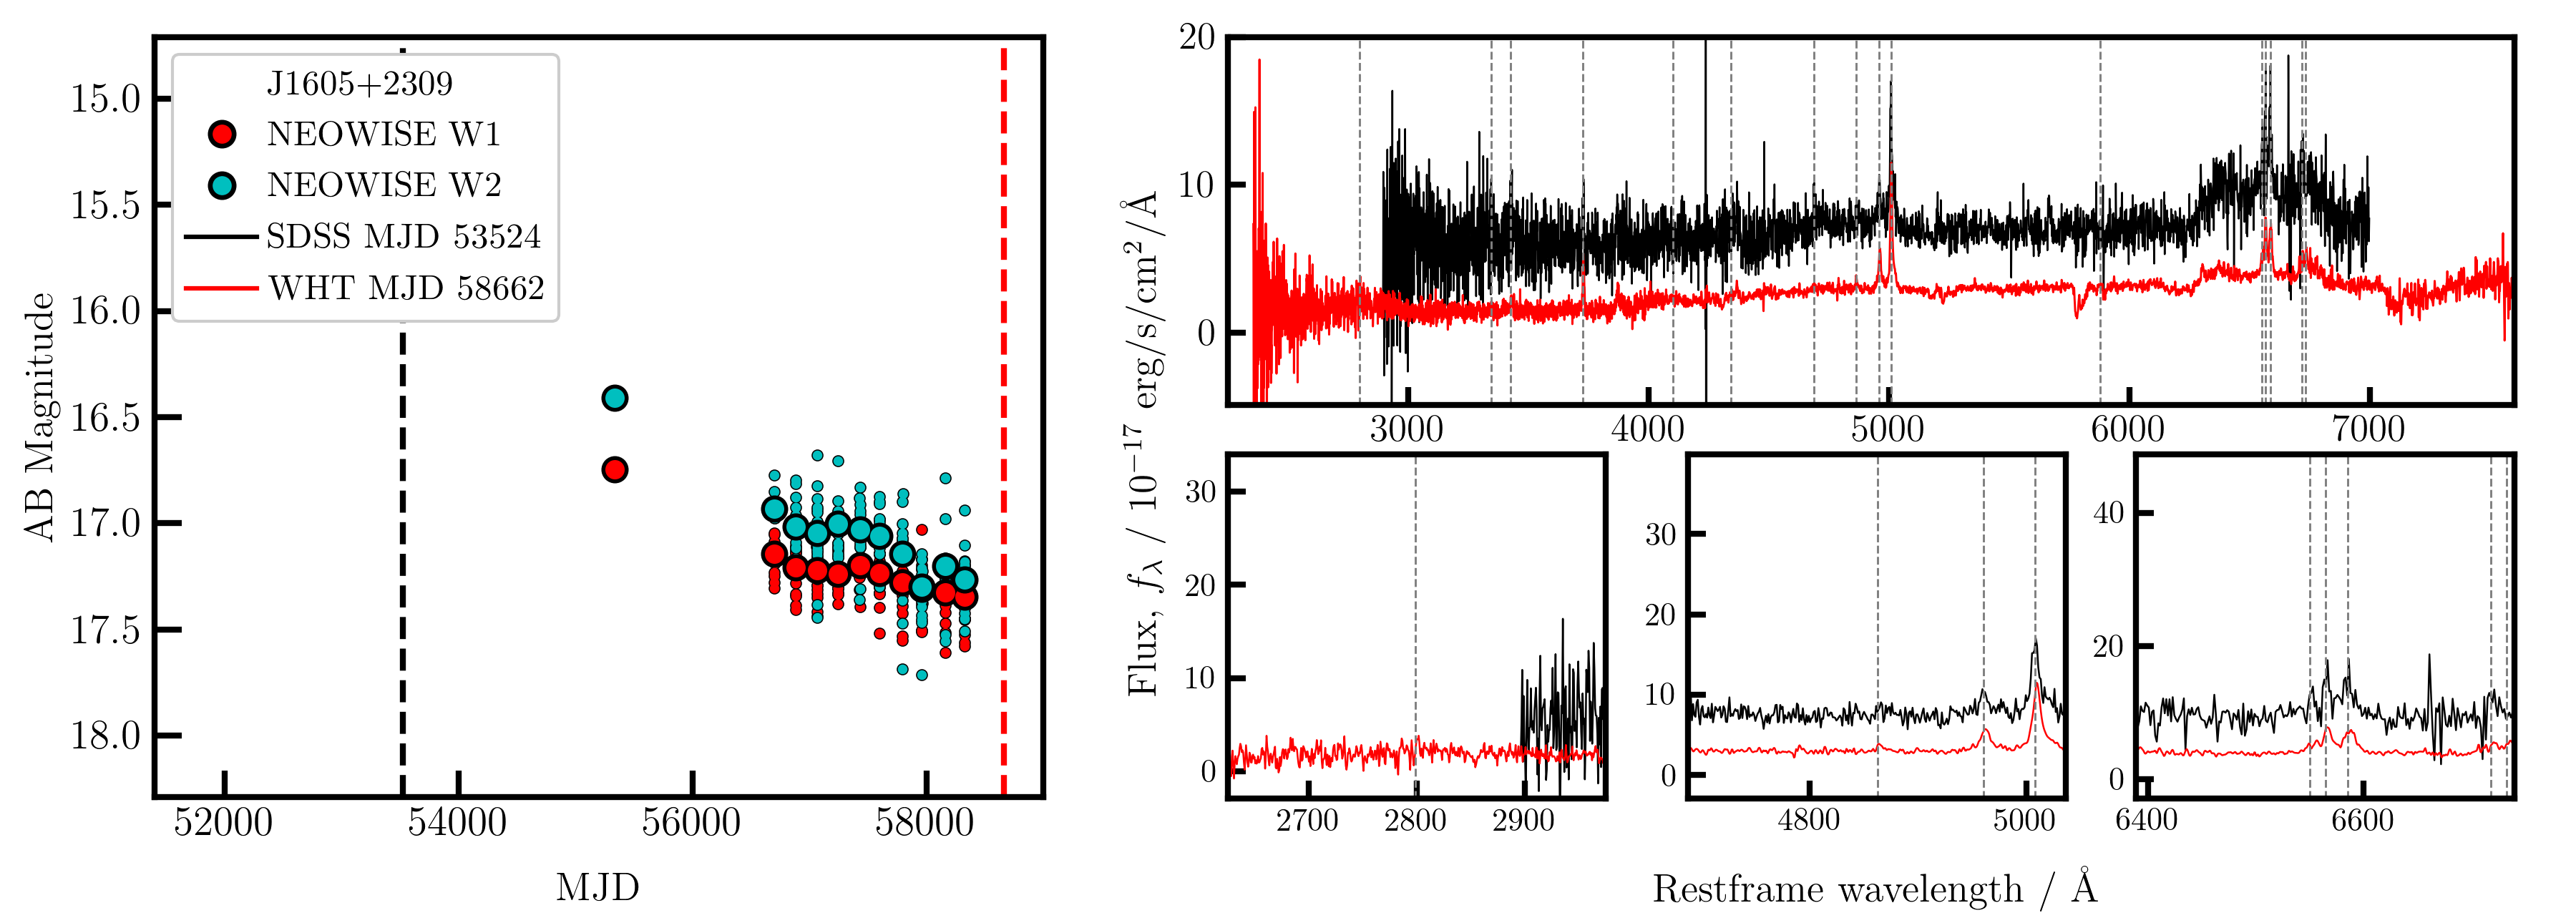
\includegraphics[width=16.7cm, trim=0.0cm 0.05cm 0.2cm 0.1cm, clip]
  {../plots/LCs_and_spectra/J1605+2309_landscape_temp.png}
  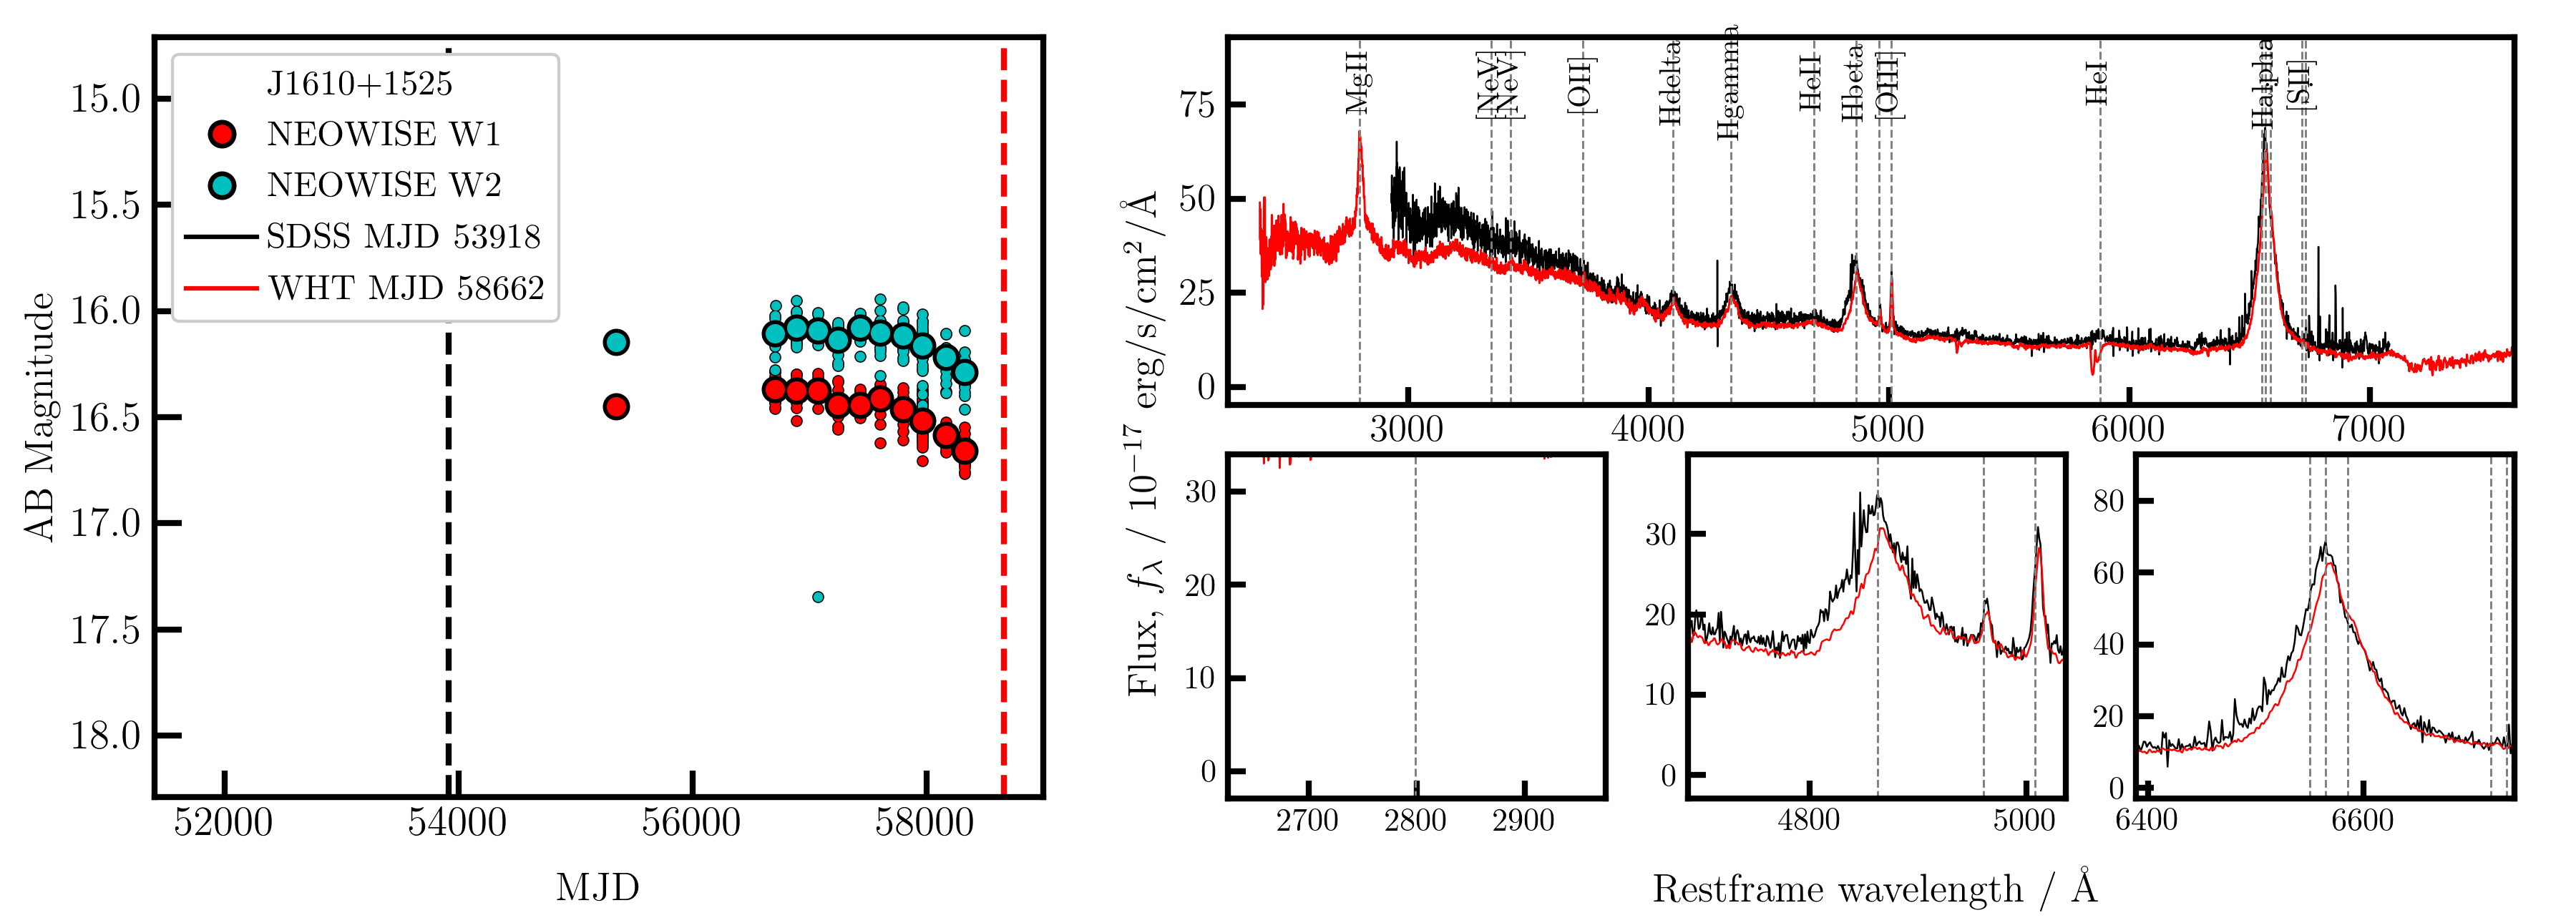
\includegraphics[width=16.7cm, trim=0.0cm 0.05cm 0.2cm 0.1cm, clip]
  {../plots/LCs_and_spectra/J1610+1525_landscape_temp.png}
    \vspace{-12pt}
  \caption[]{}
  \label{fig:all_spectra_b}
\end{figure*}

\begin{figure*}
  \centering
  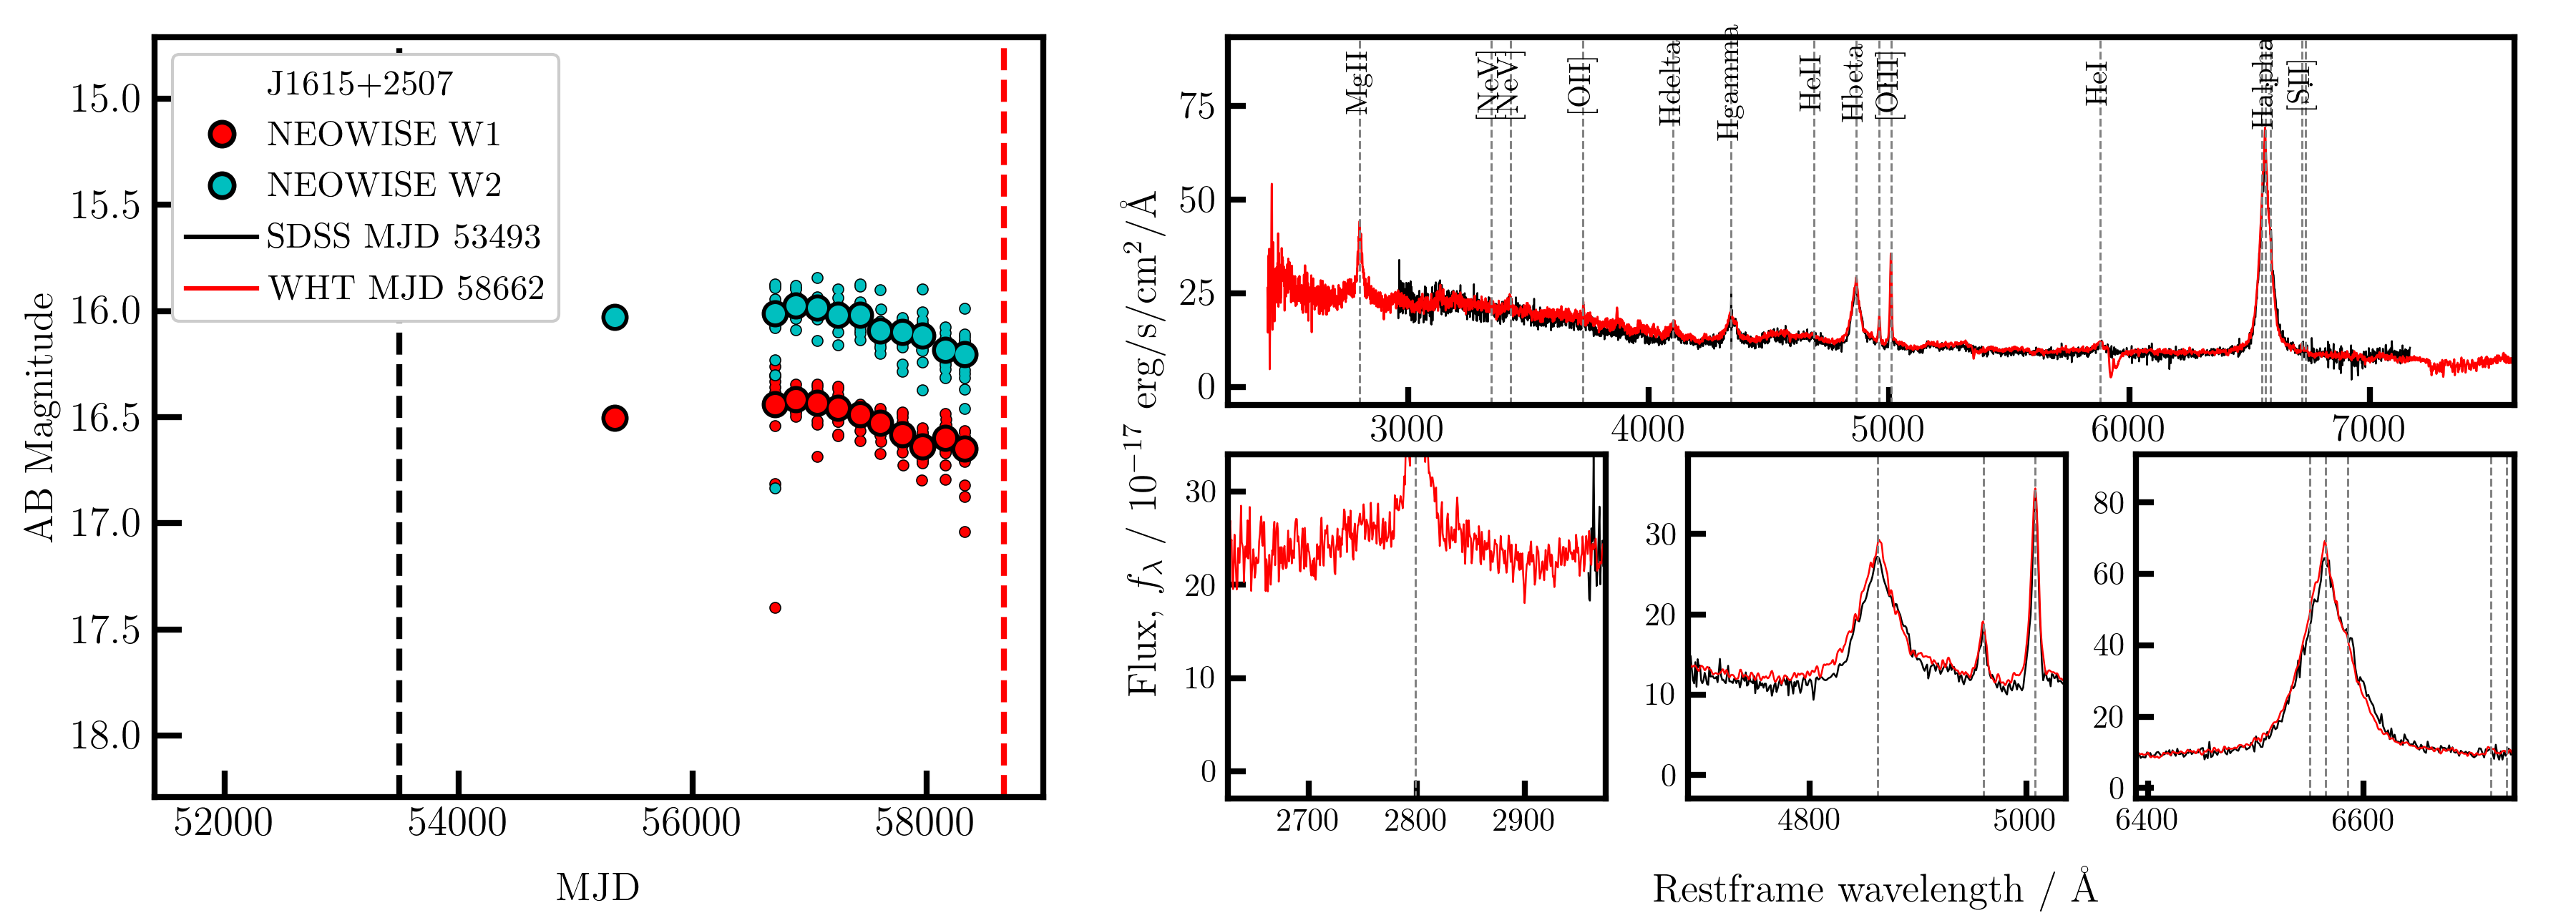
\includegraphics[width=16.7cm, trim=0.0cm 0.05cm 0.2cm 0.1cm, clip]
  {../plots/LCs_and_spectra/J1615+2507_landscape_temp.png}
  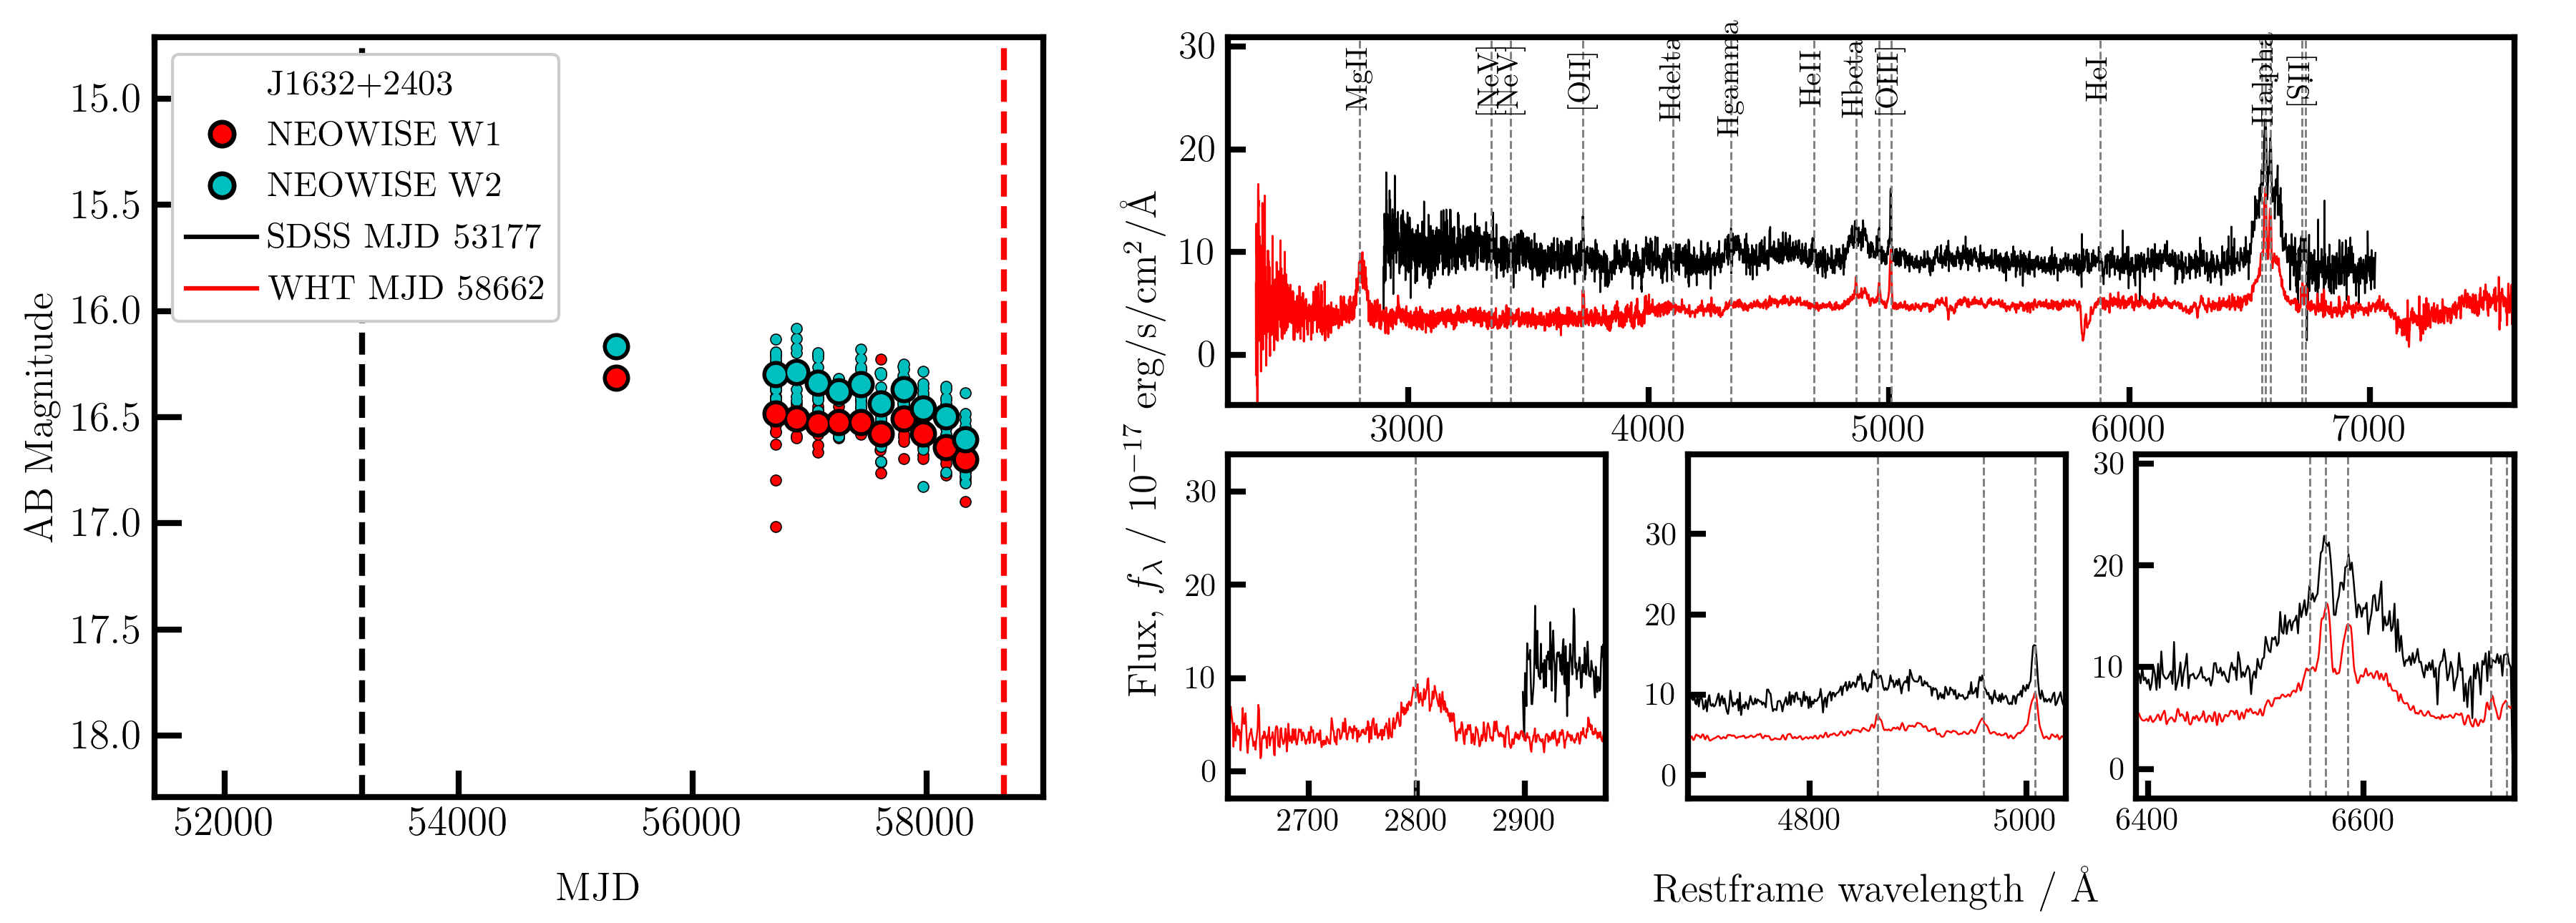
\includegraphics[width=16.7cm, trim=0.0cm 0.05cm 0.2cm 0.1cm, clip]
  {../plots/LCs_and_spectra/J1632+2403_landscape_temp.png}
  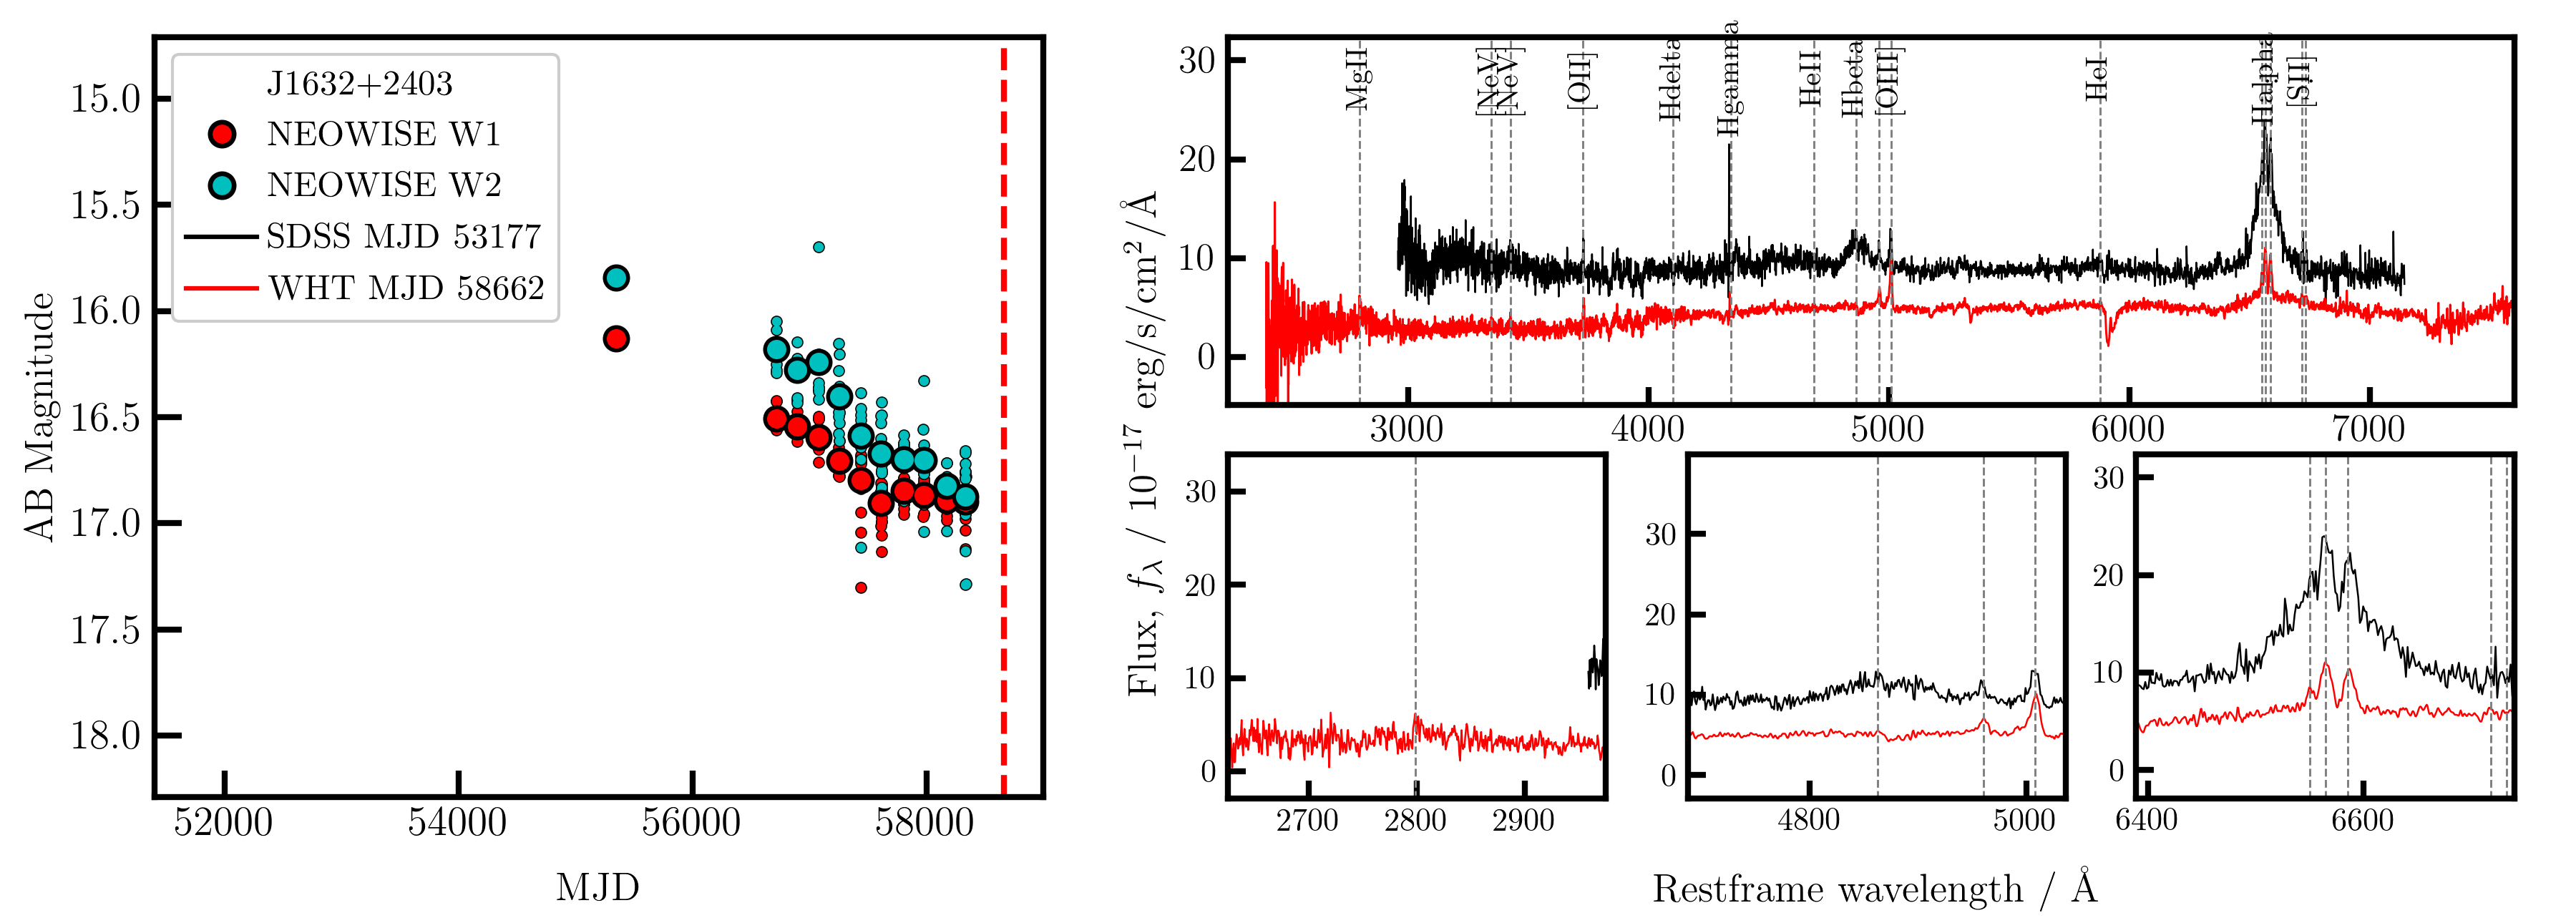
\includegraphics[width=16.7cm, trim=0.0cm 0.05cm 0.2cm 0.1cm, clip]
  {../plots/LCs_and_spectra/J1634+1118_landscape_temp.png}        
  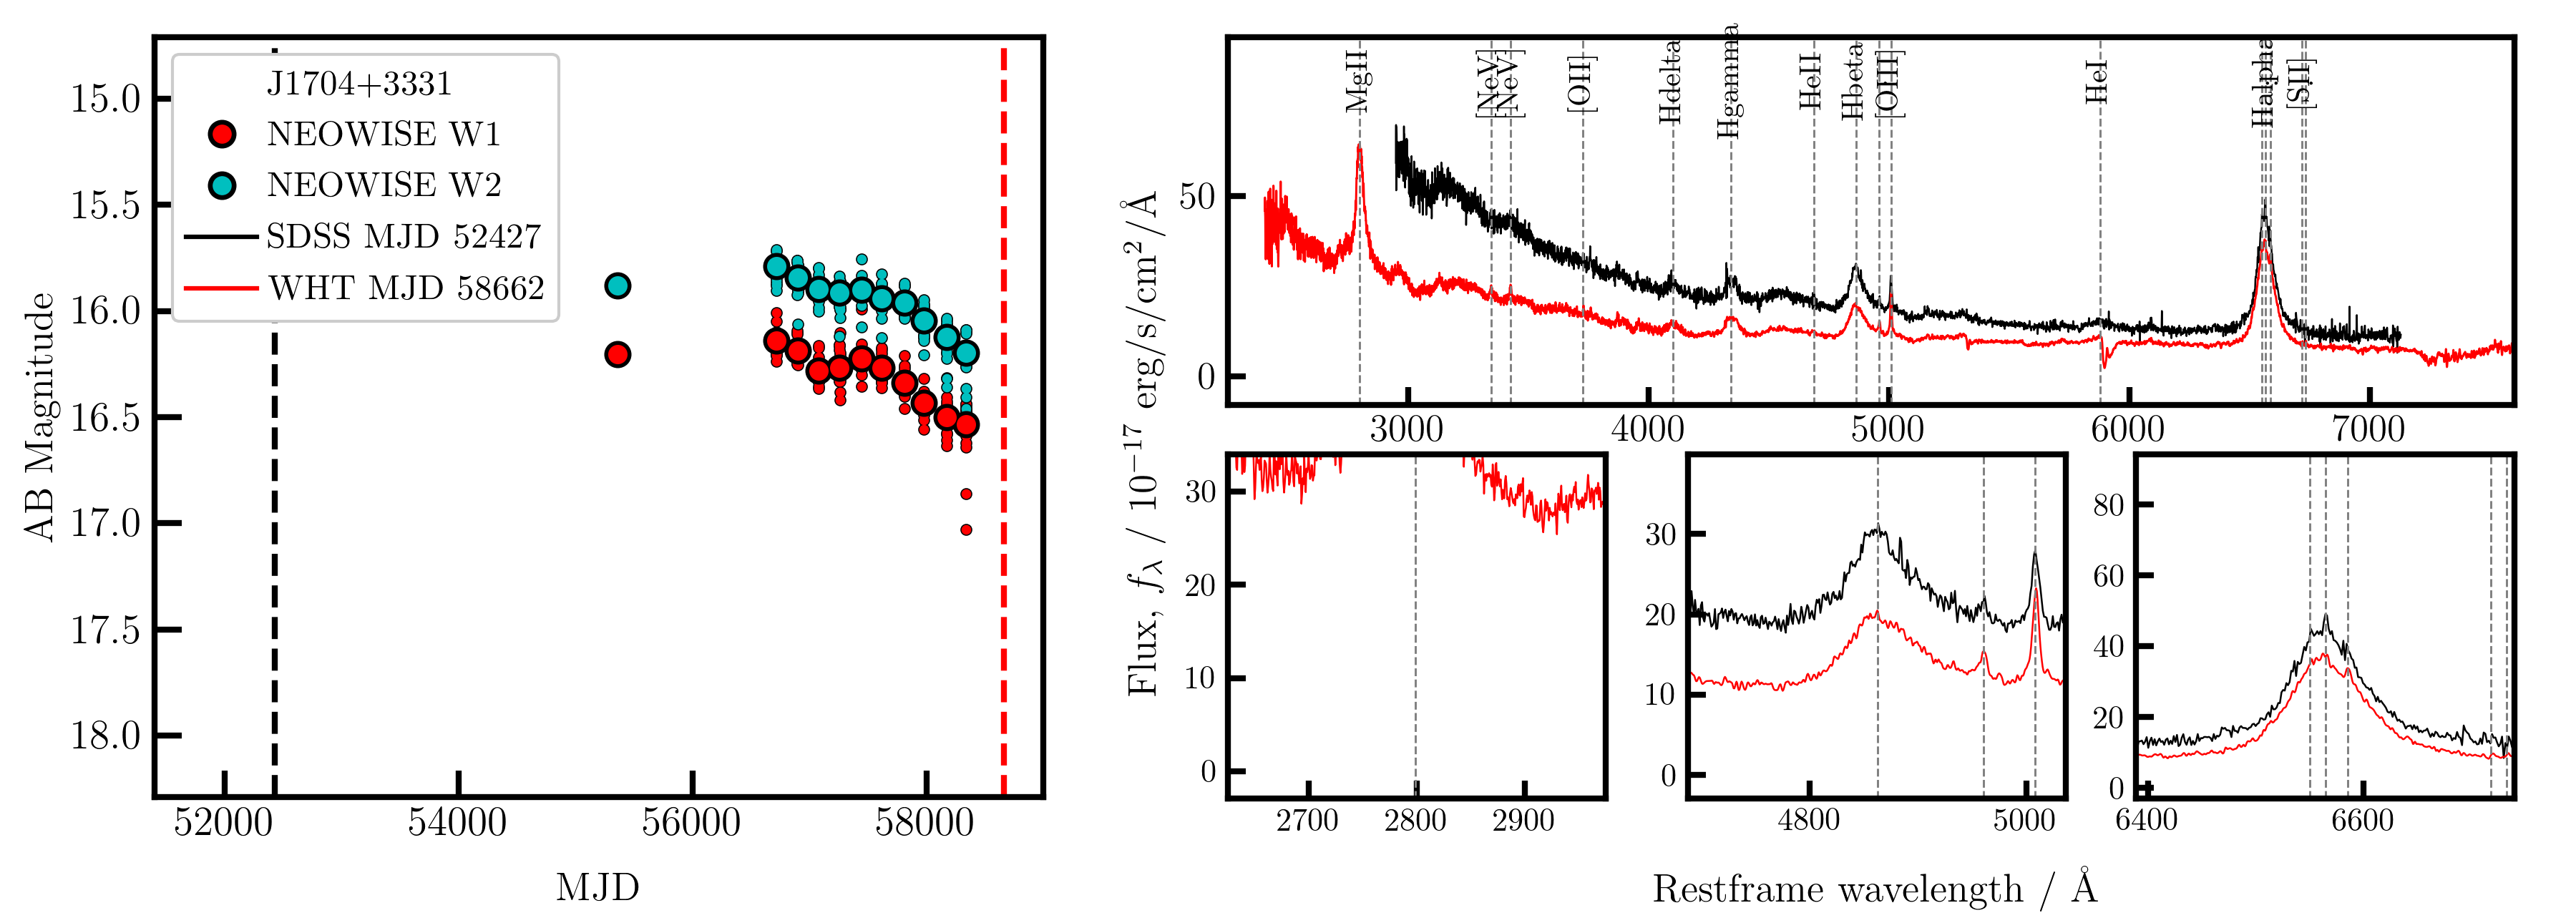
\includegraphics[width=16.7cm, trim=0.0cm 0.05cm 0.2cm 0.1cm, clip]
  {../plots/LCs_and_spectra/J1704+3331_landscape_temp.png}
    \vspace{-12pt}
  \caption[]{}
  \label{fig:all_spectra_c}
\end{figure*}

\begin{figure*}
  \centering
  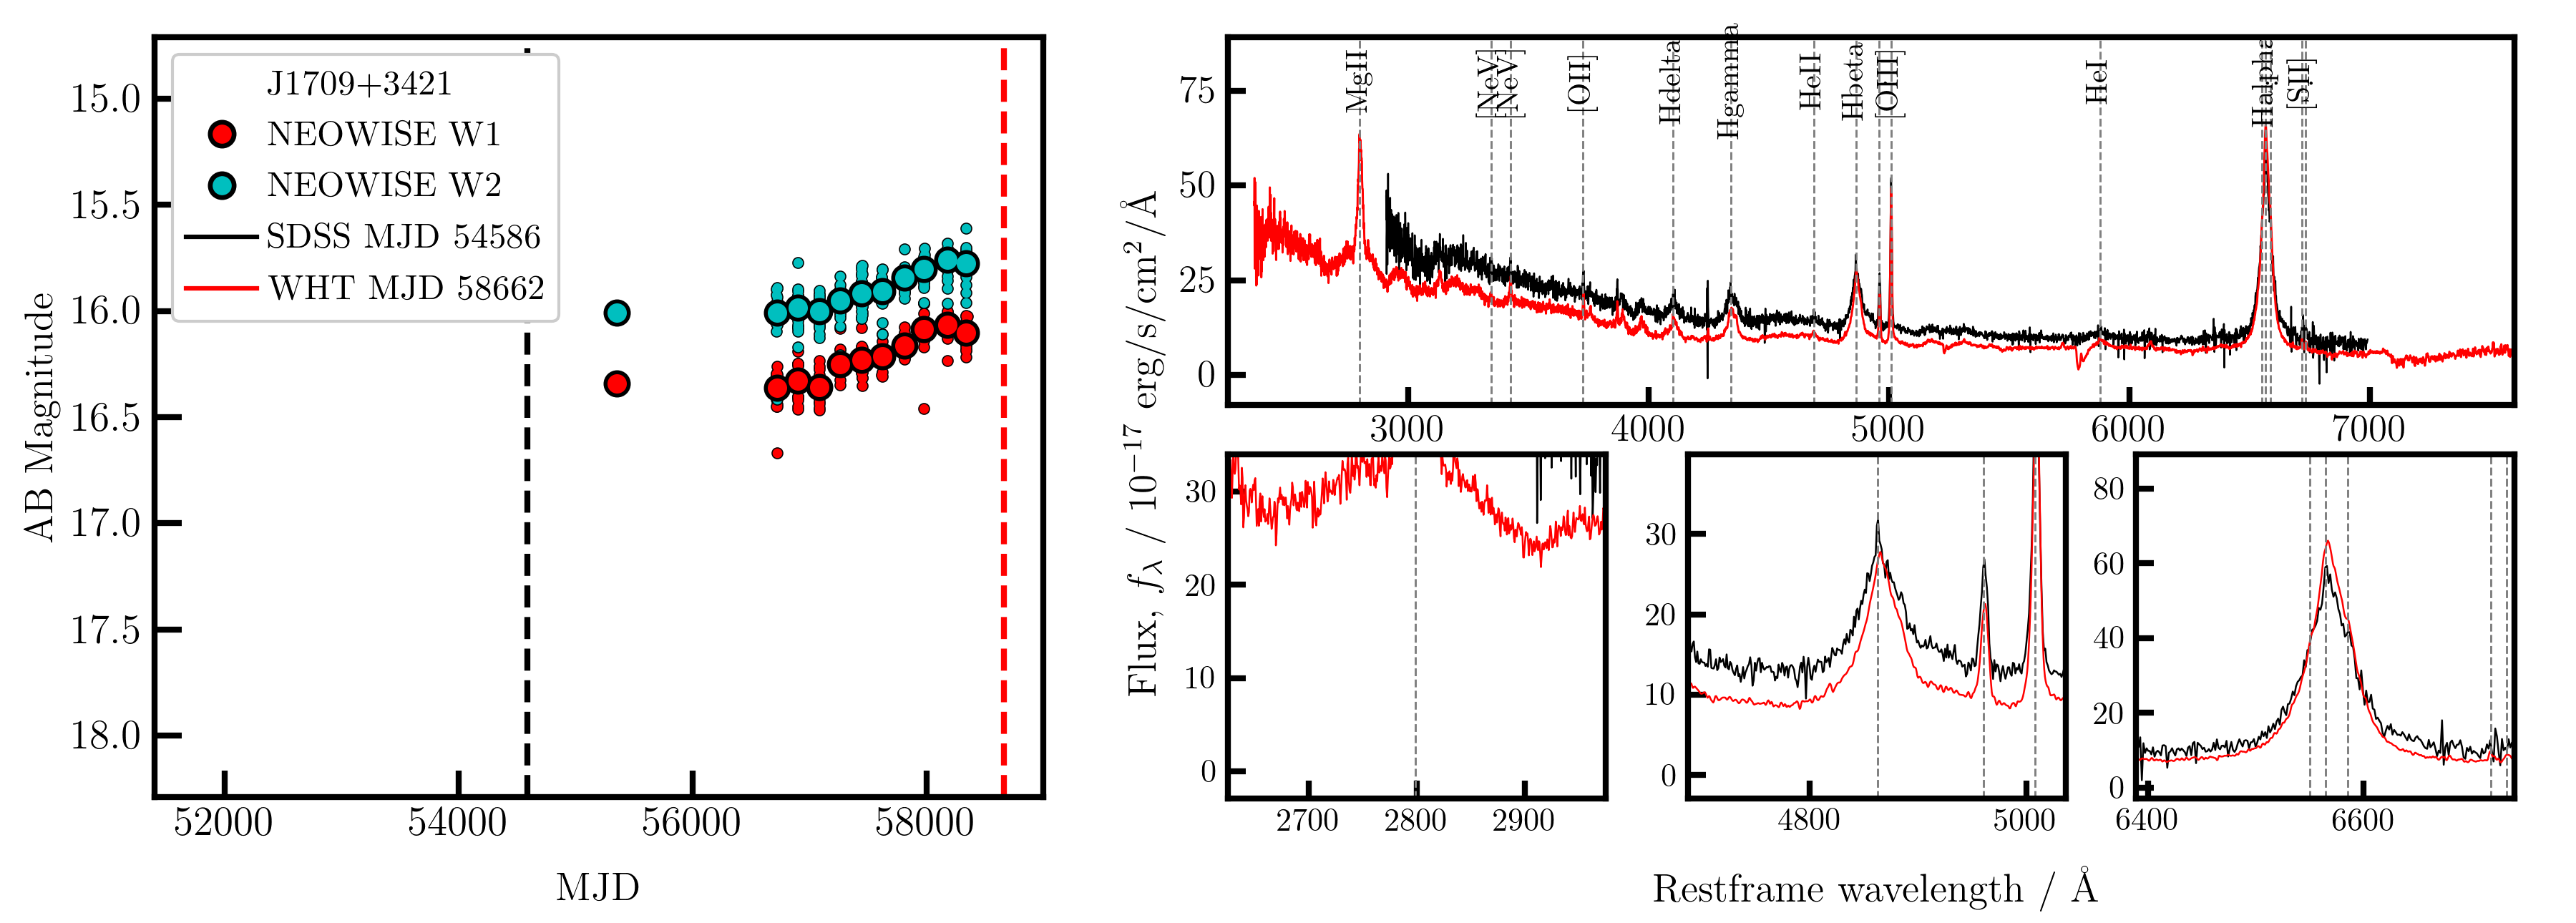
\includegraphics[width=16.7cm, trim=0.0cm 0.05cm 0.2cm 0.1cm, clip]
   {../plots/LCs_and_spectra/J1709+3421_landscape_temp.png}
  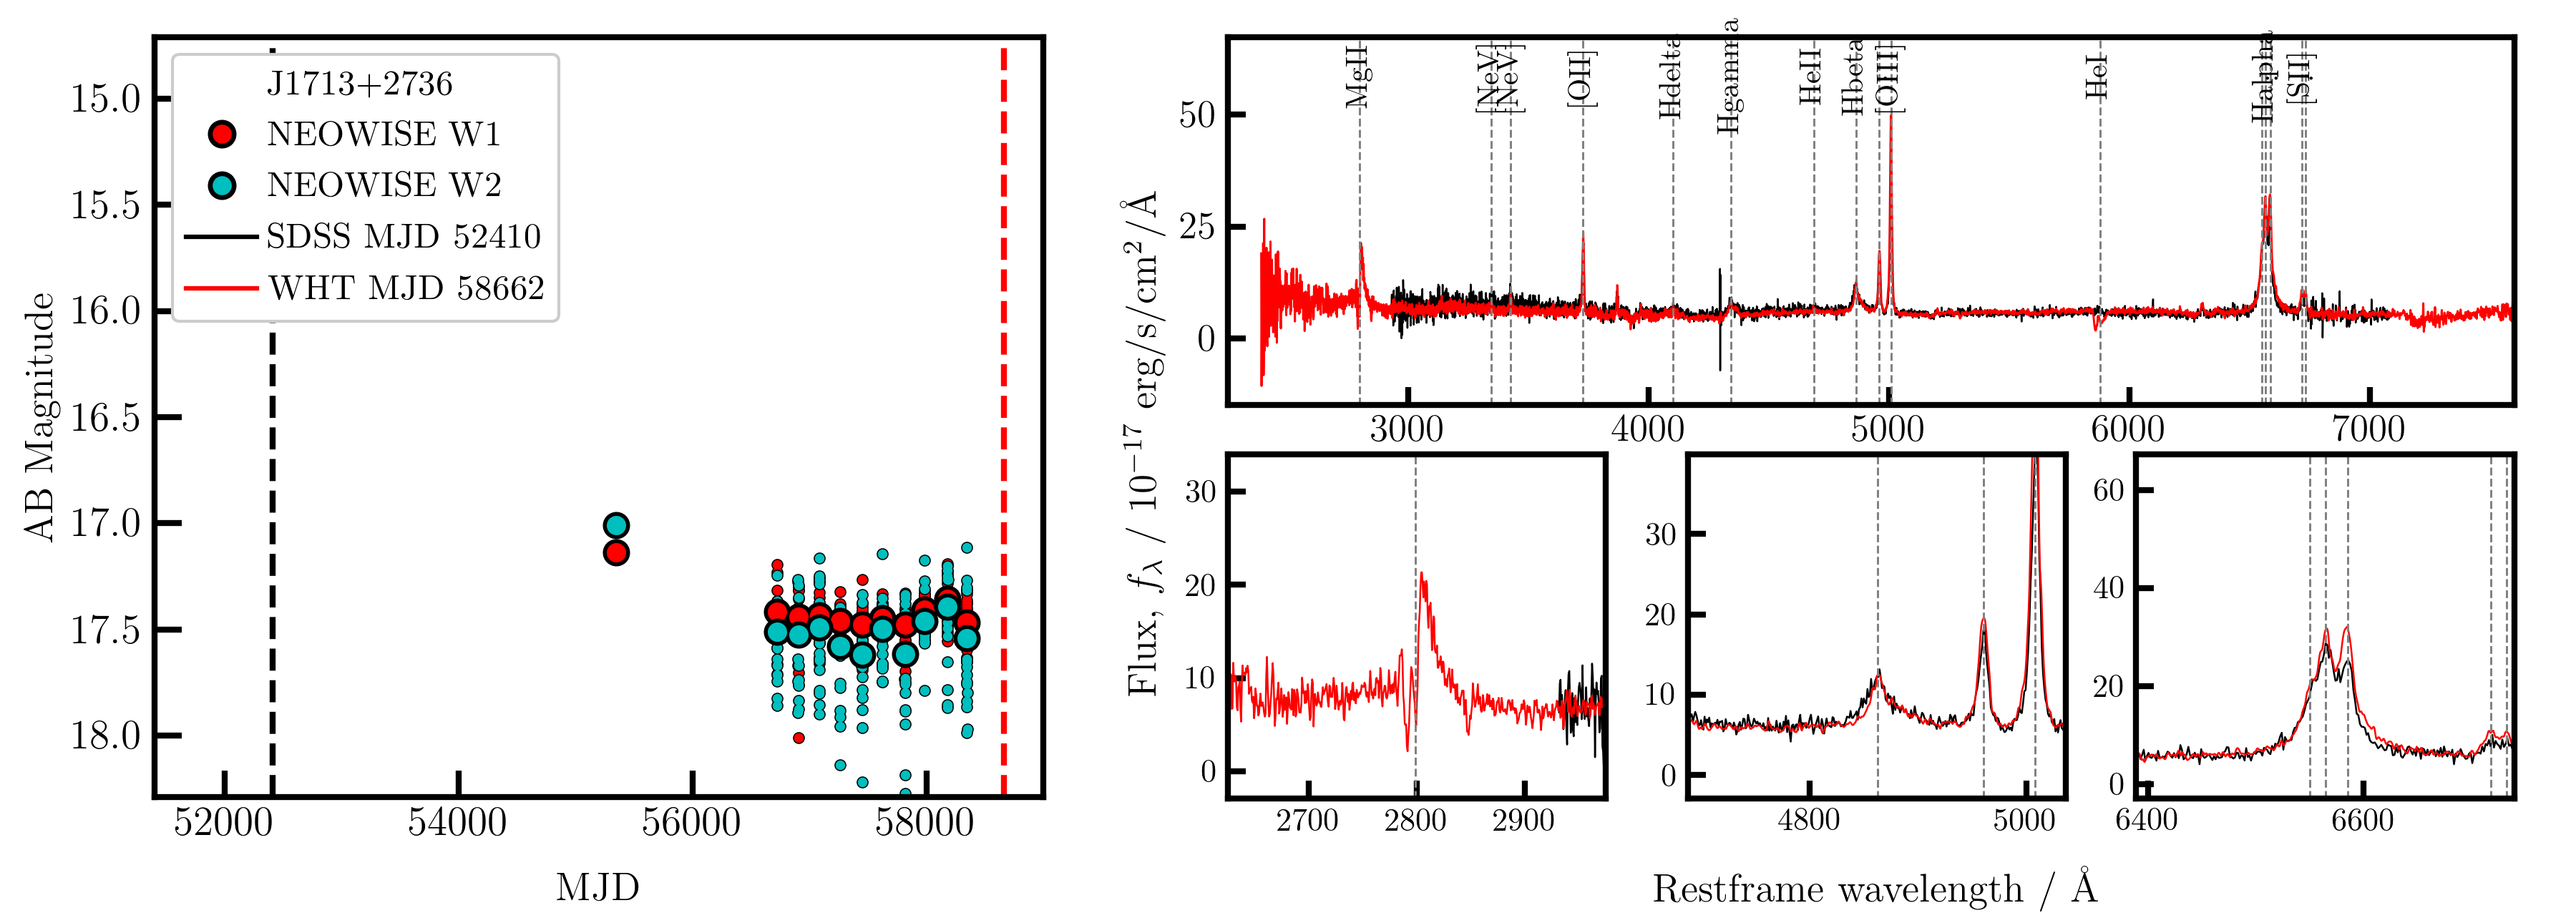
\includegraphics[width=16.7cm, trim=0.0cm 0.05cm 0.2cm 0.1cm, clip]
  {../plots/LCs_and_spectra/J1713+2736_landscape_temp.png}
  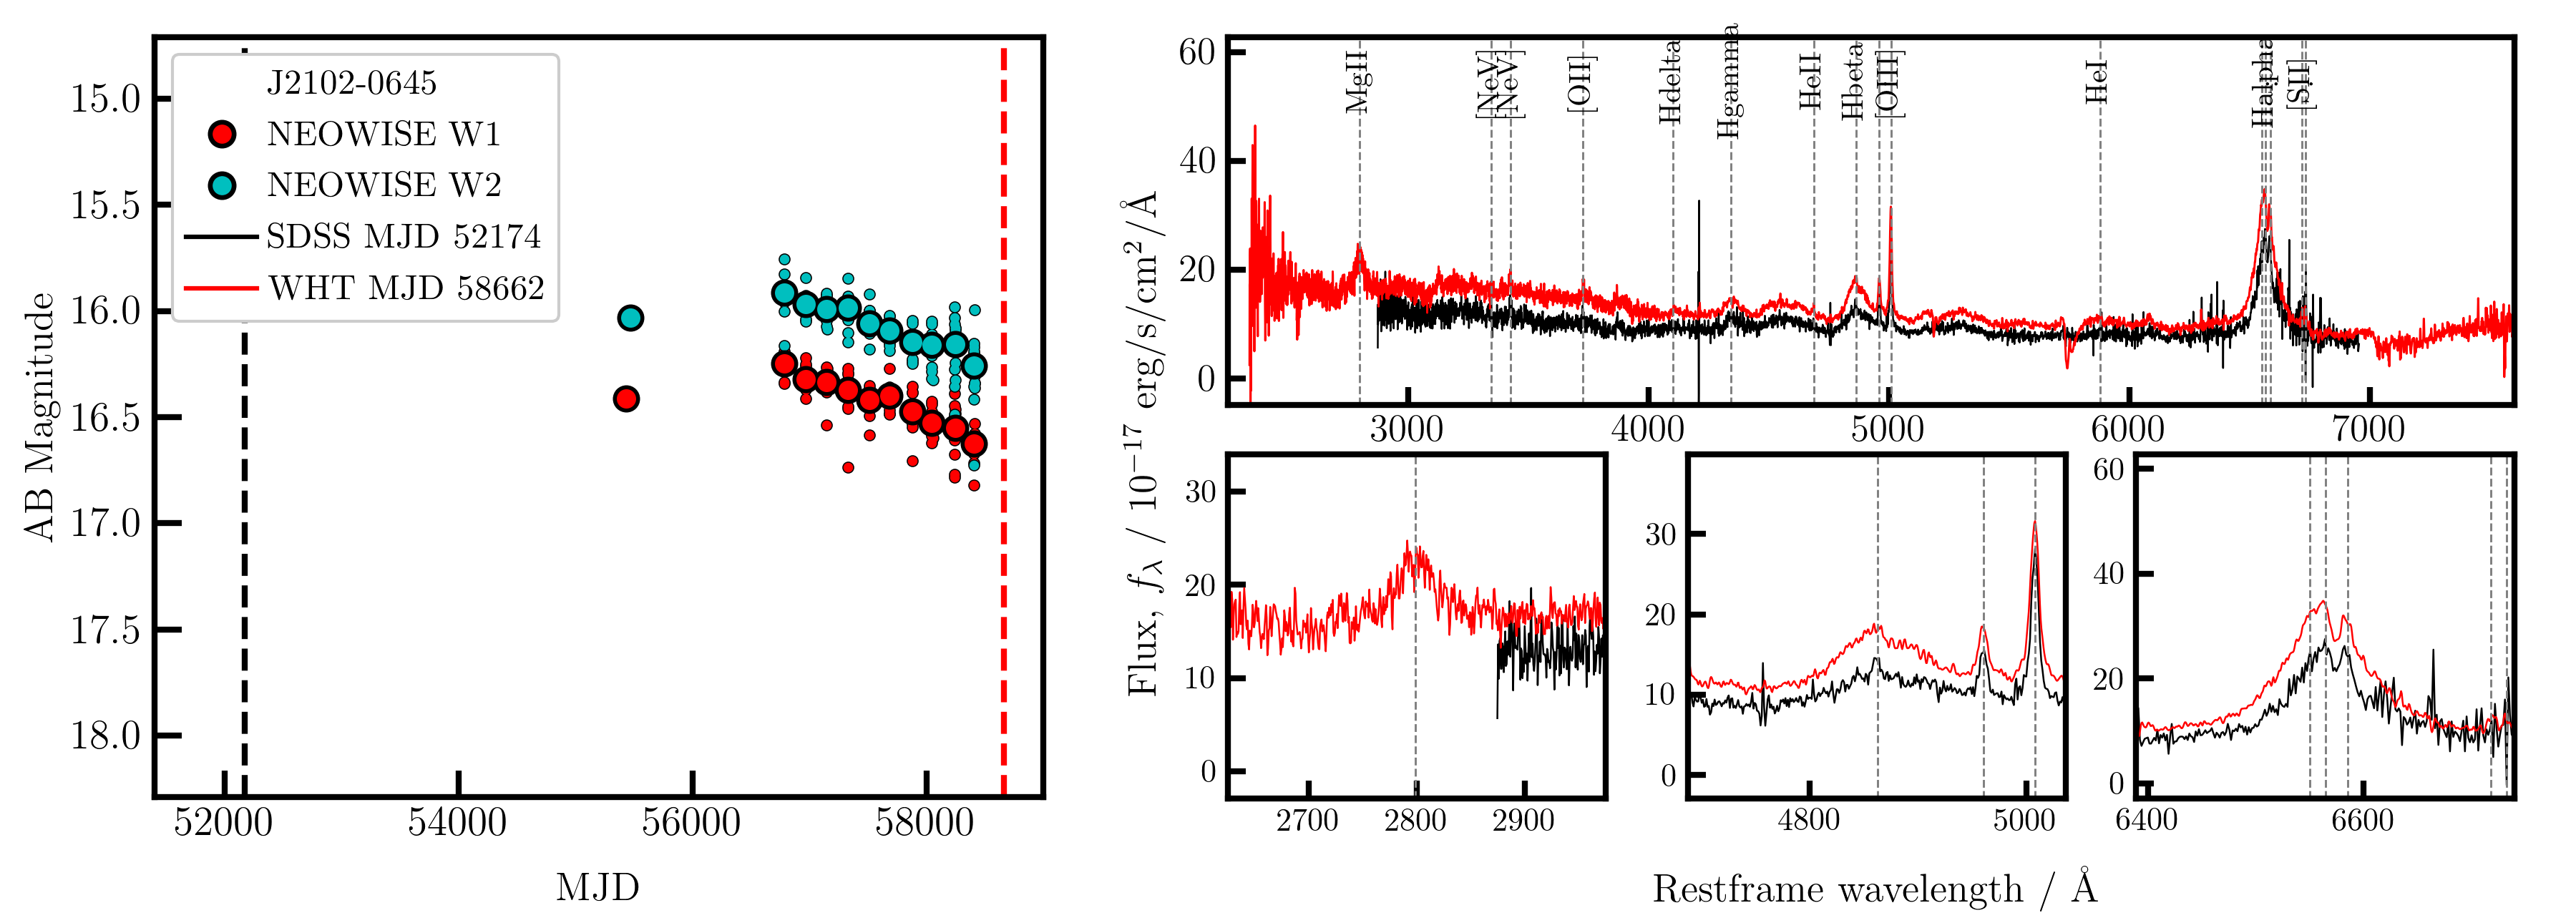
\includegraphics[width=16.7cm, trim=0.0cm 0.05cm 0.2cm 0.1cm, clip]
  {../plots/LCs_and_spectra/J2102-0645_landscape_temp.png}
  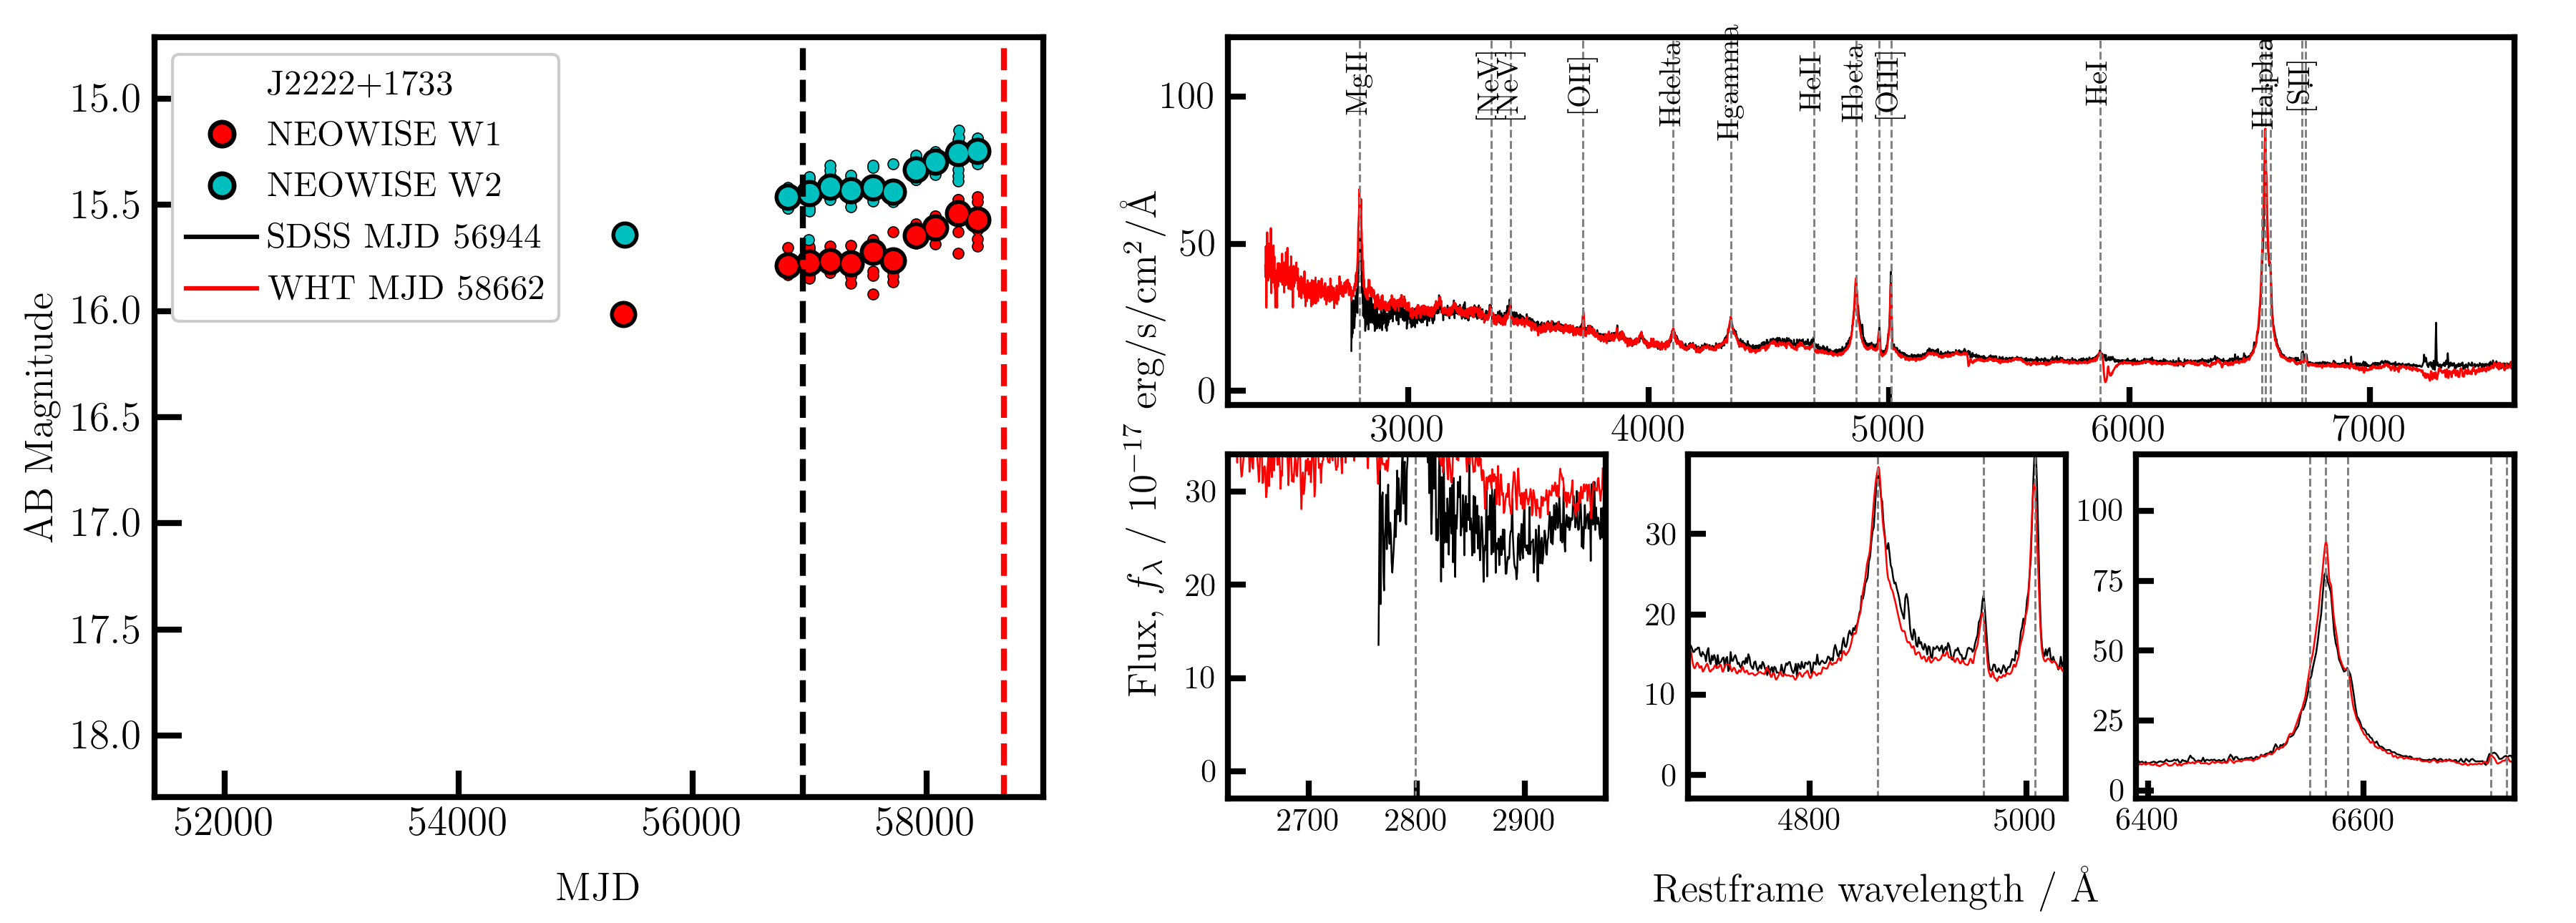
\includegraphics[width=16.7cm, trim=0.0cm 0.05cm 0.2cm 0.1cm, clip]
  {../plots/LCs_and_spectra/J2222+1733_landscape_temp.png}
    \vspace{-12pt}
  \caption[]{}
  \label{fig:all_spectra_d}
\end{figure*}

\begin{figure*}
  \centering
  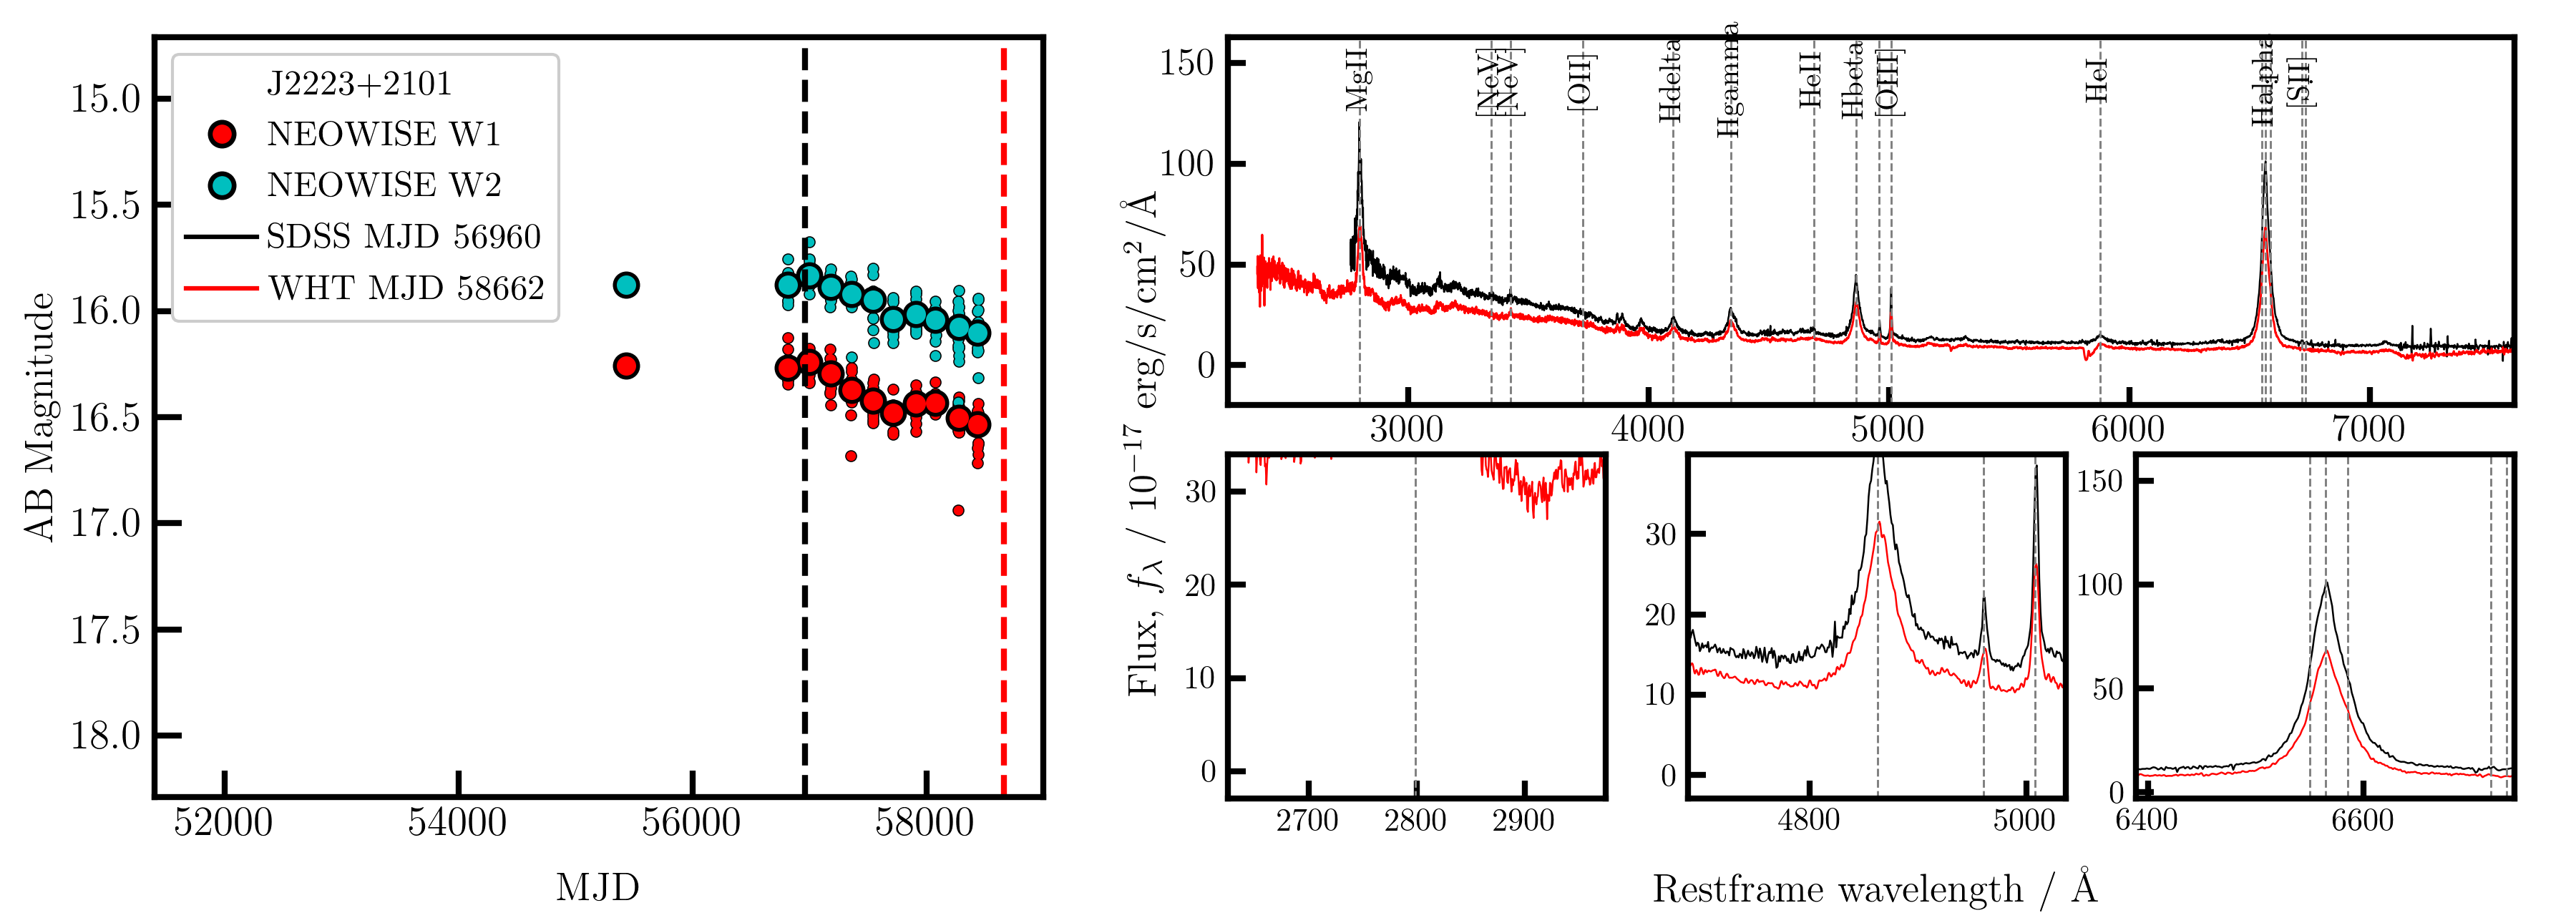
\includegraphics[width=16.7cm, trim=0.0cm 0.05cm 0.2cm 0.1cm, clip]
  {../plots/LCs_and_spectra/J2223+2101_landscape_temp.png}
  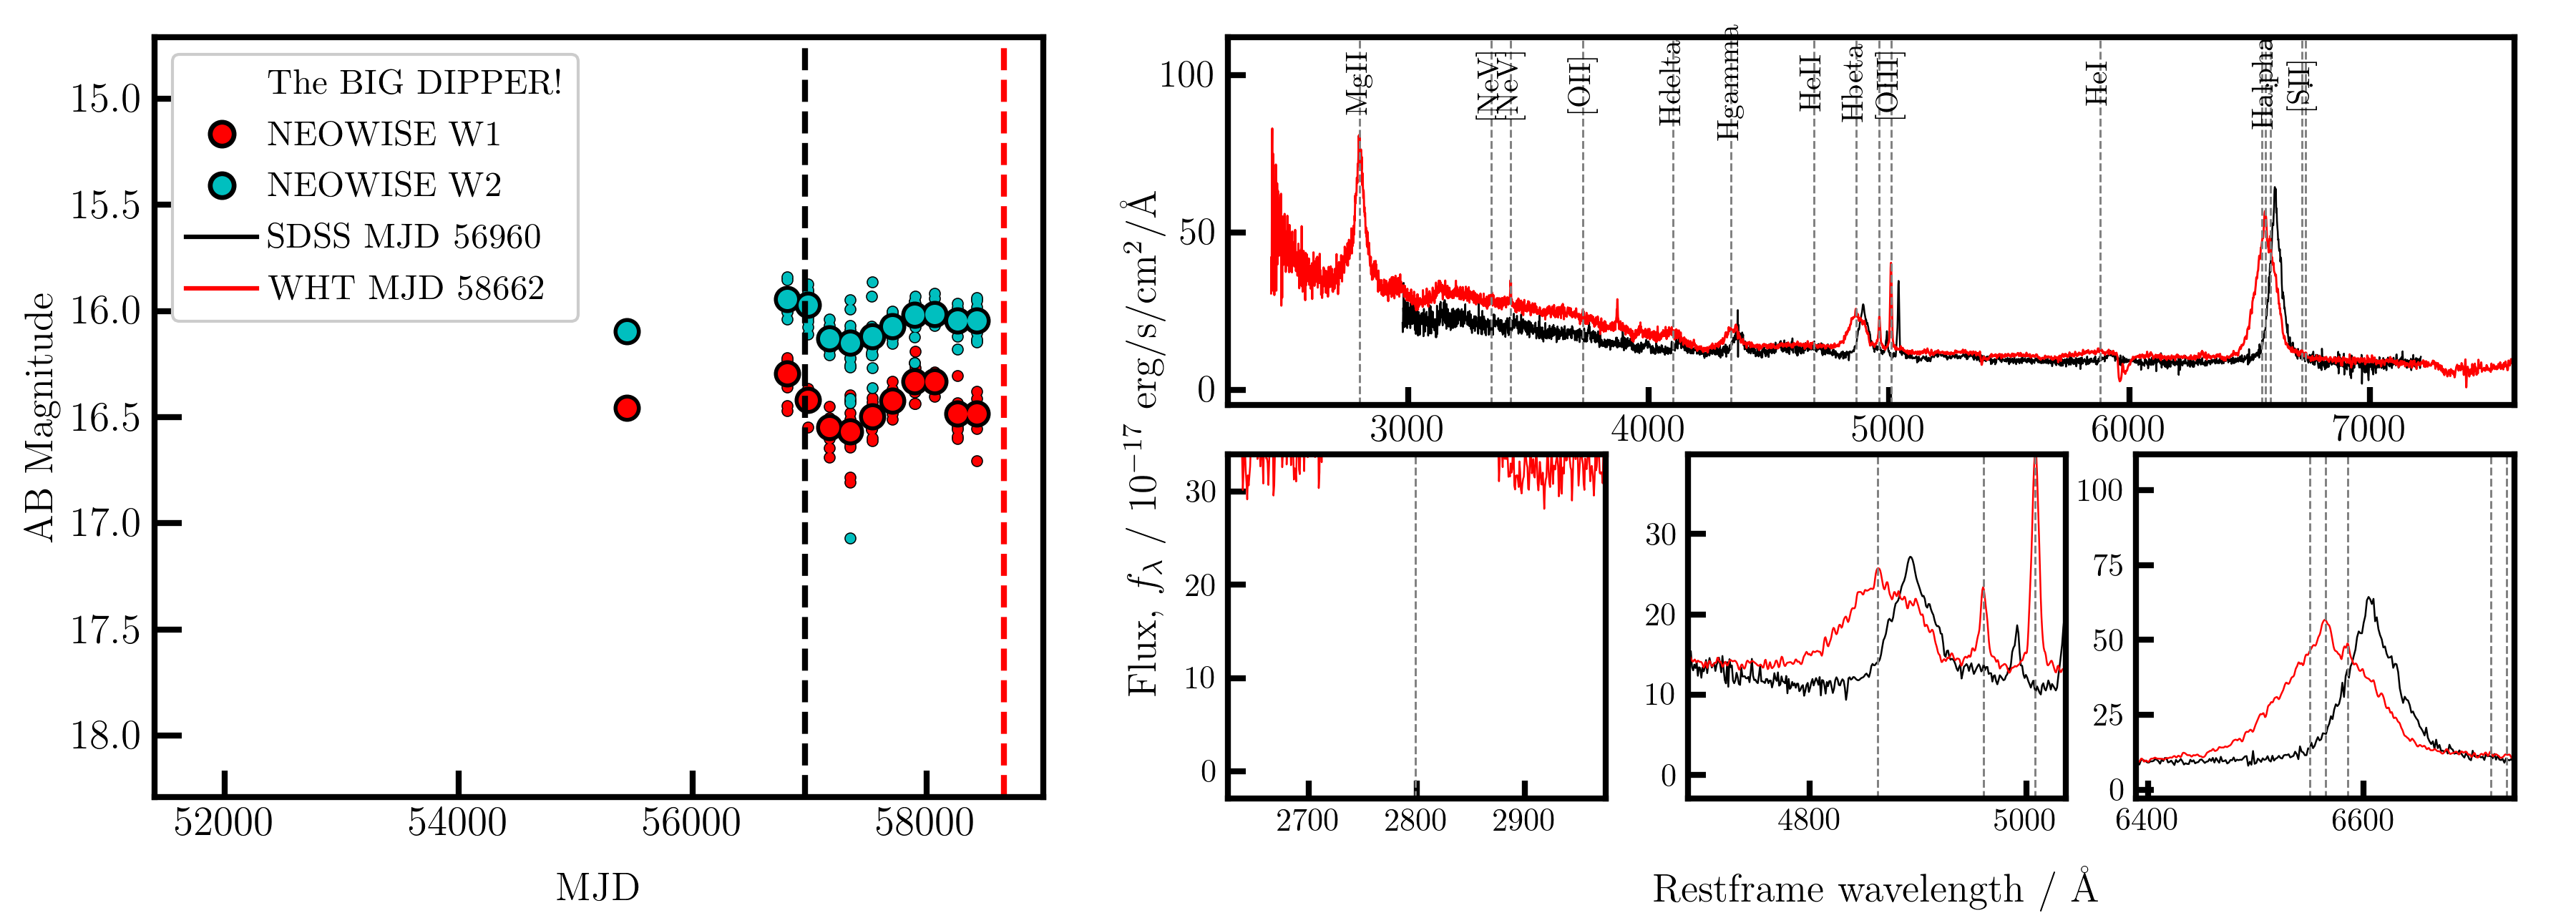
\includegraphics[width=16.7cm, trim=0.0cm 0.05cm 0.2cm 0.1cm, clip]
  {../plots/LCs_and_spectra/J2232-0806_landscape_temp.png}
  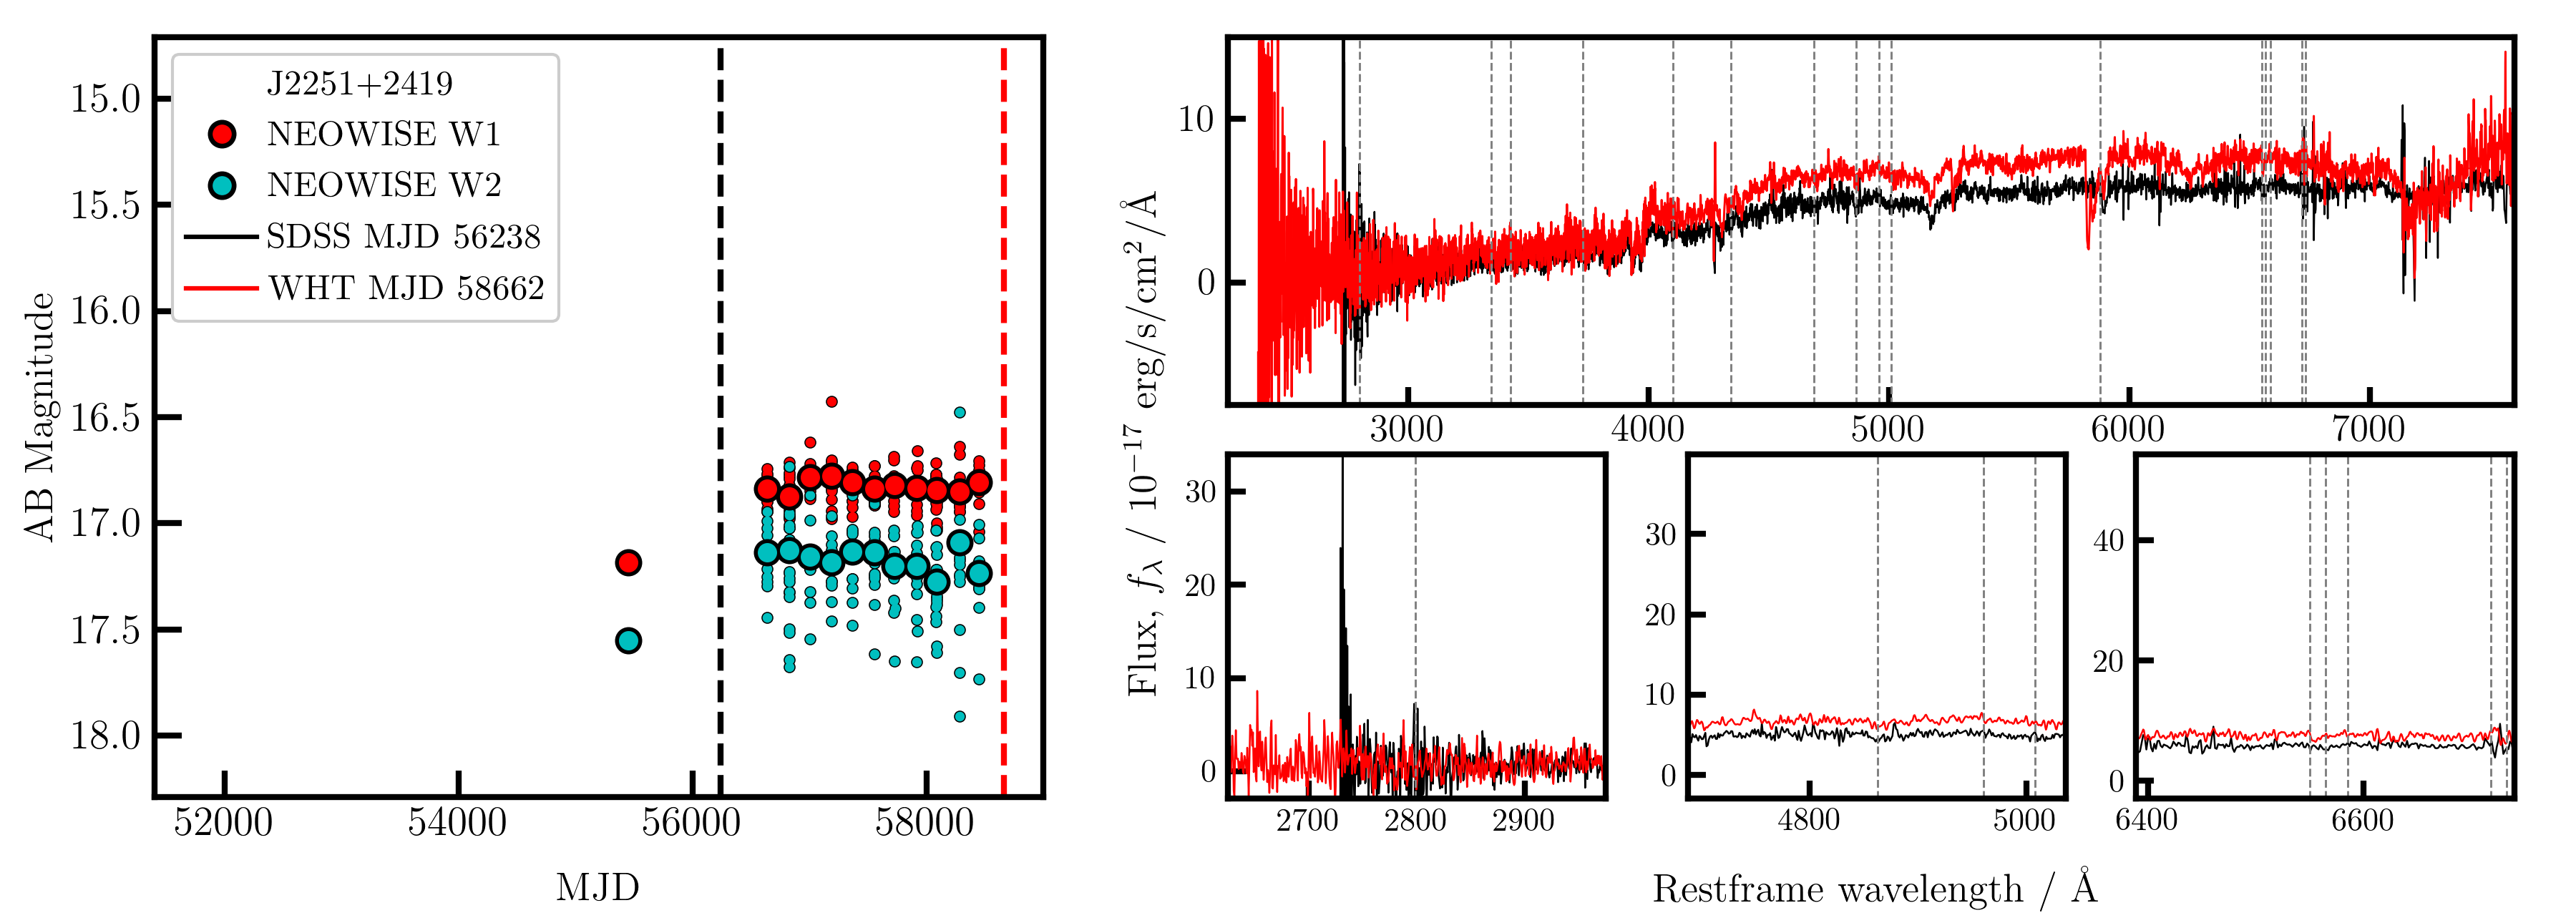
\includegraphics[width=16.7cm, trim=0.0cm 0.05cm 0.2cm 0.1cm, clip]
  {../plots/LCs_and_spectra/J2251+2419_landscape_temp.png}
    \vspace{-12pt}
  \caption[]{}
  \label{fig:all_spectra_e}
\end{figure*}

\begin{figure*}
  \centering
    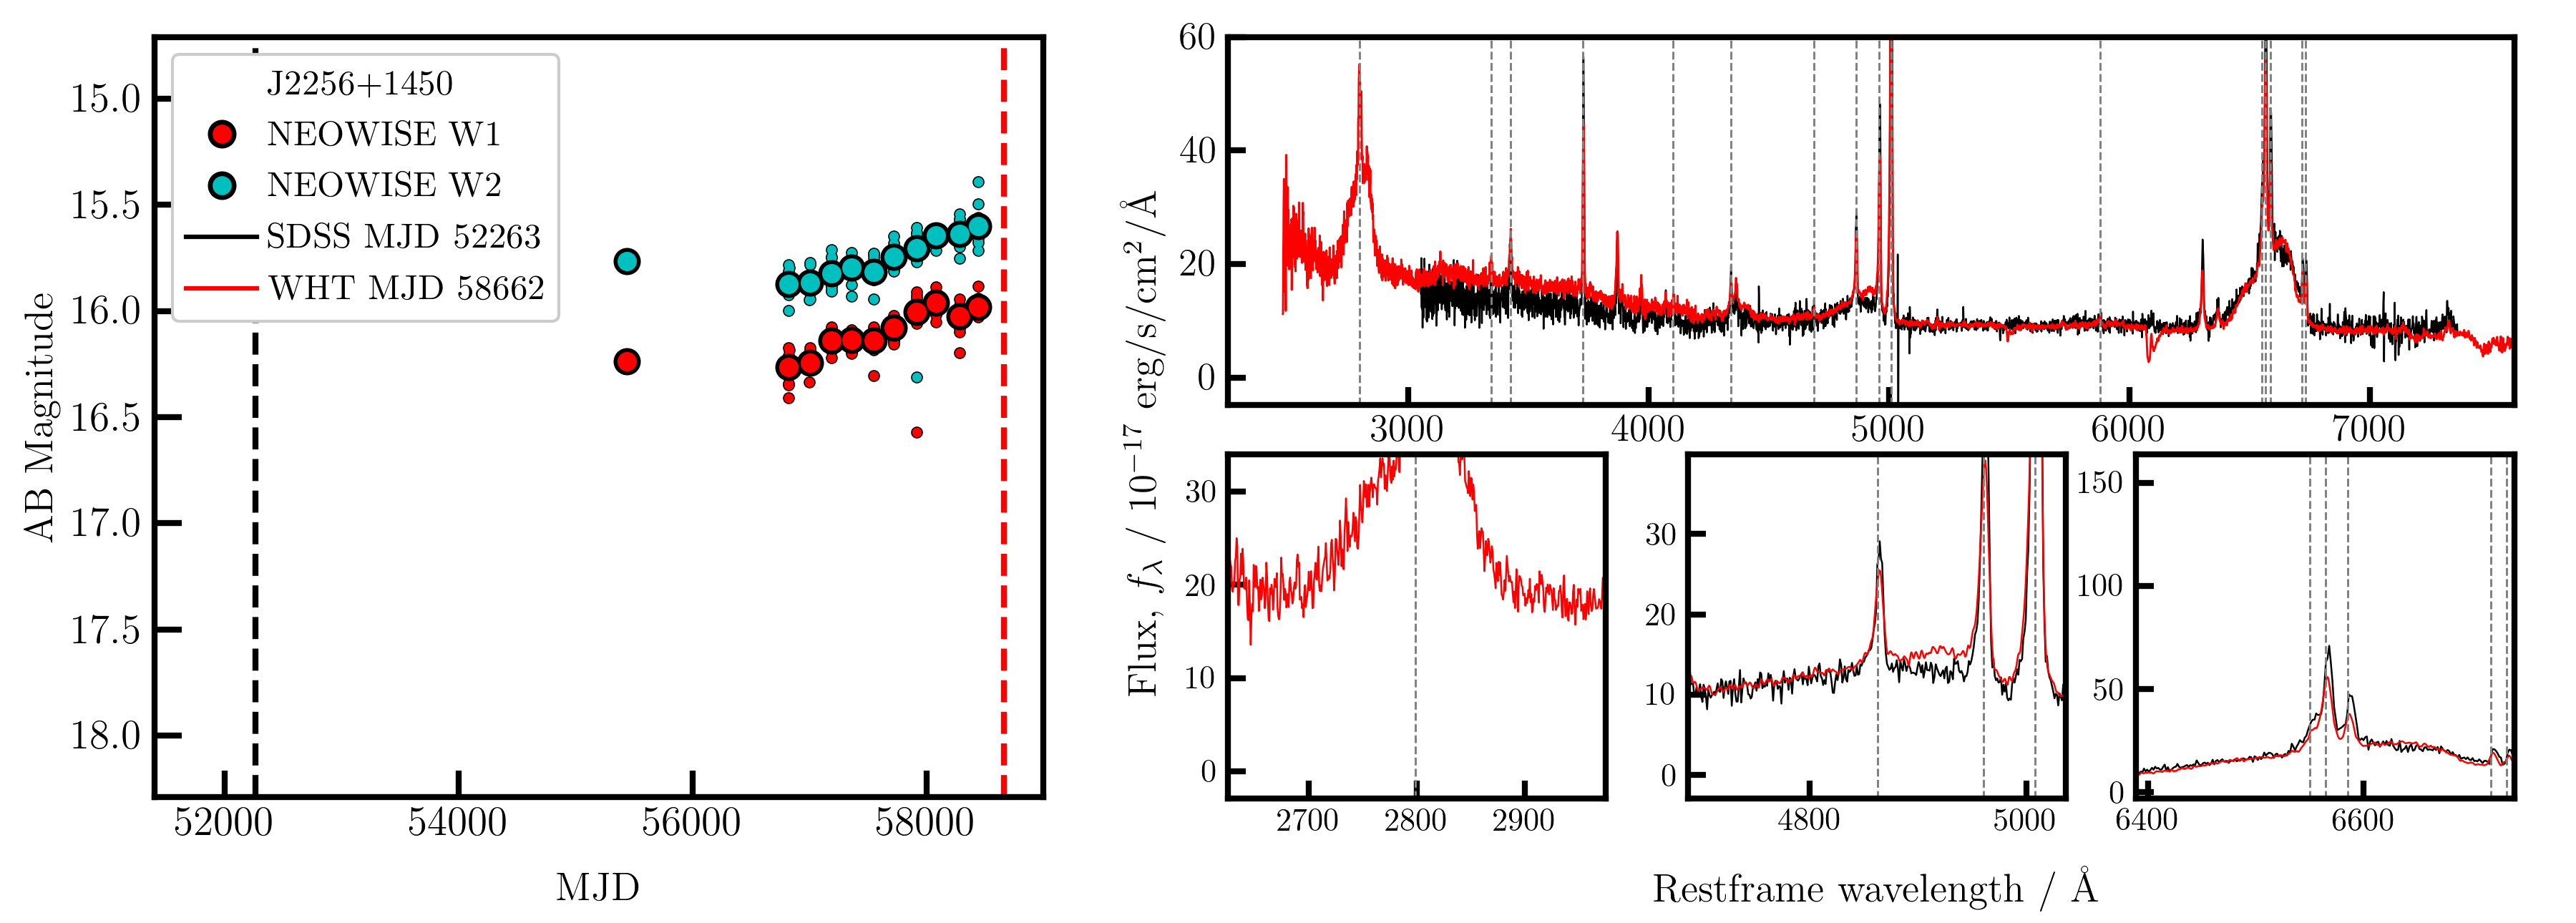
\includegraphics[width=16.7cm, trim=0.0cm 0.05cm 0.2cm 0.1cm, clip]
  {../plots/LCs_and_spectra/J2256+1450_landscape_temp.png}
  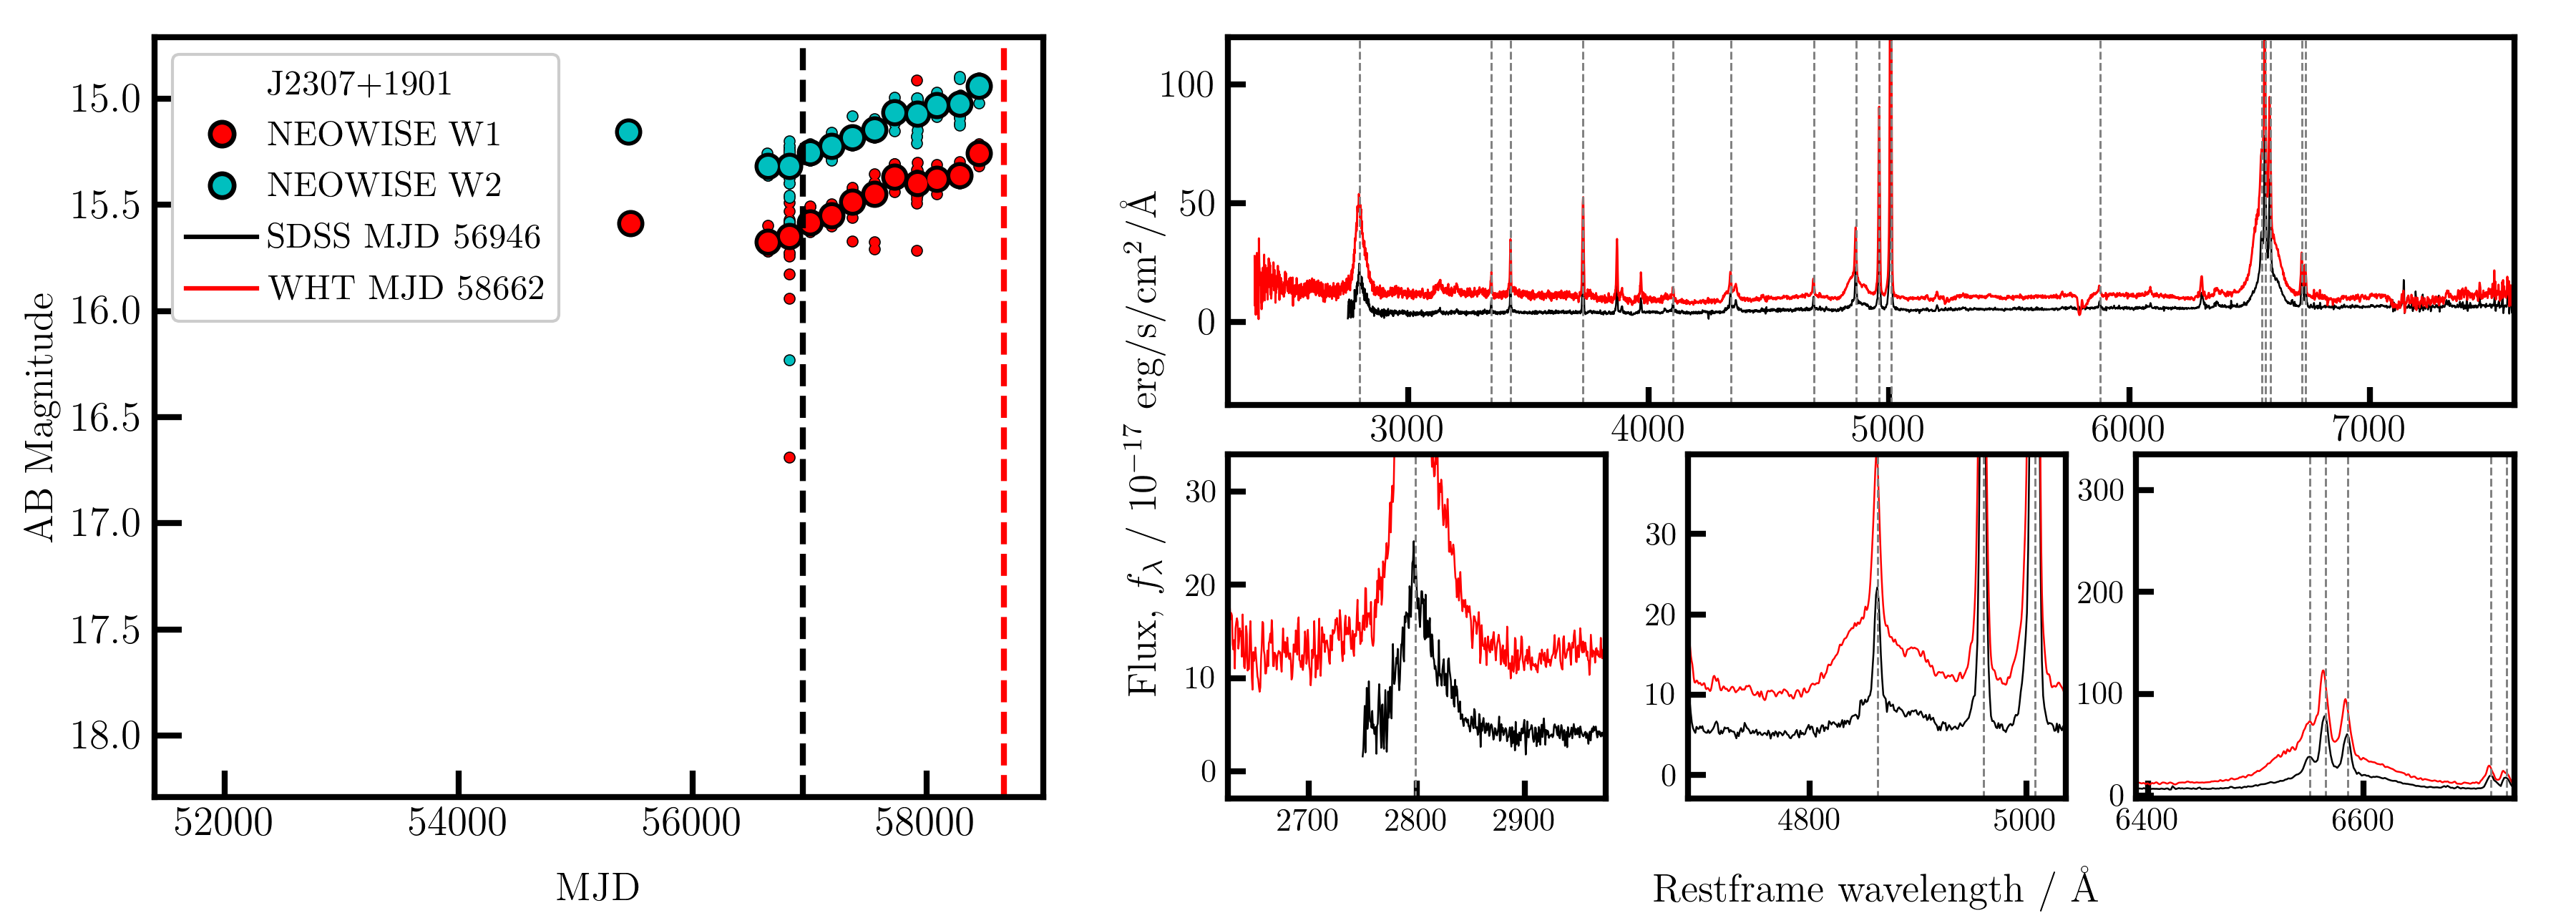
\includegraphics[width=16.7cm, trim=0.0cm 0.05cm 0.2cm 0.1cm, clip]
  {../plots/LCs_and_spectra/J2307+1901_landscape_temp.png}
    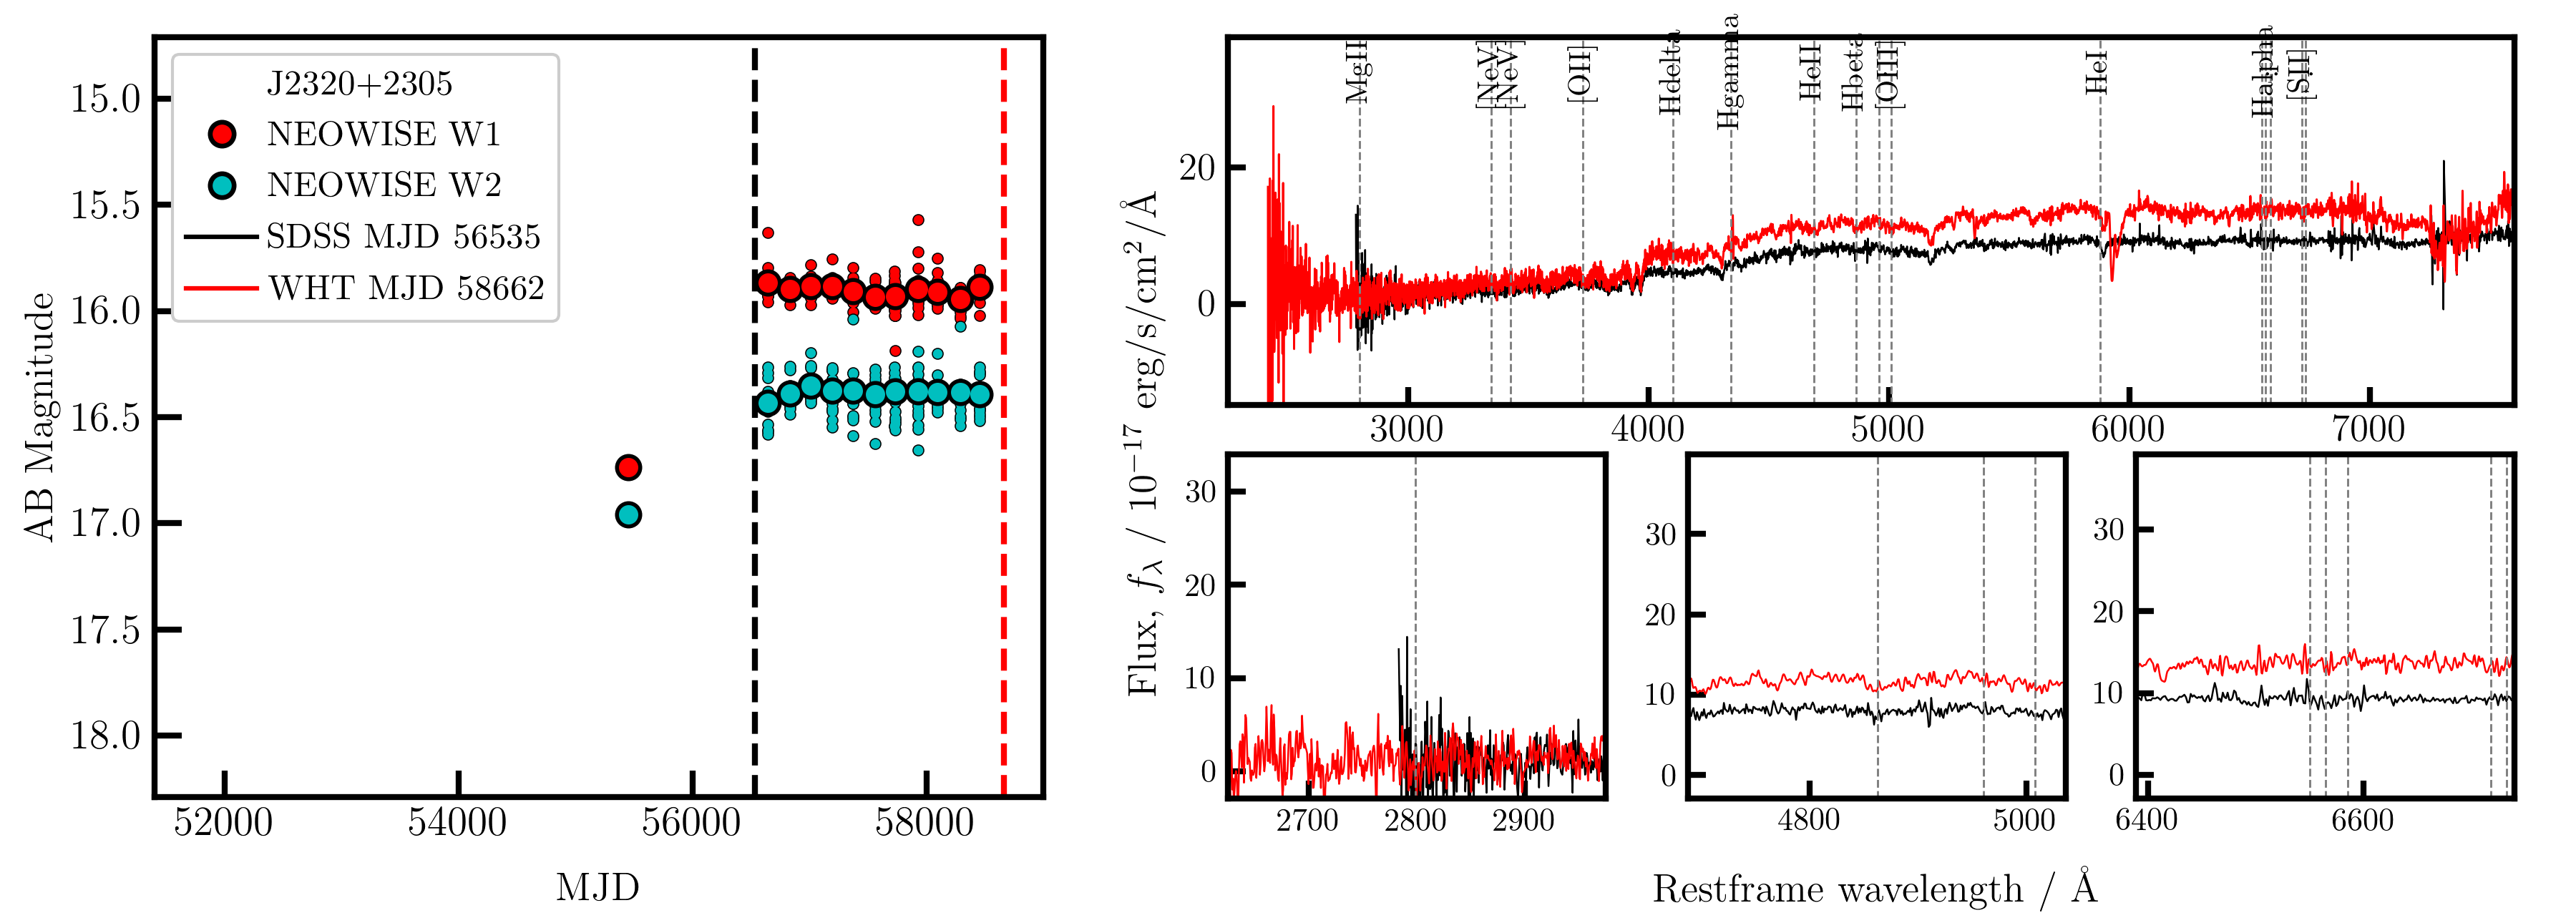
\includegraphics[width=16.7cm, trim=0.0cm 0.05cm 0.2cm 0.1cm, clip]
    {../plots/LCs_and_spectra/J2320+2305_landscape_temp.png}
      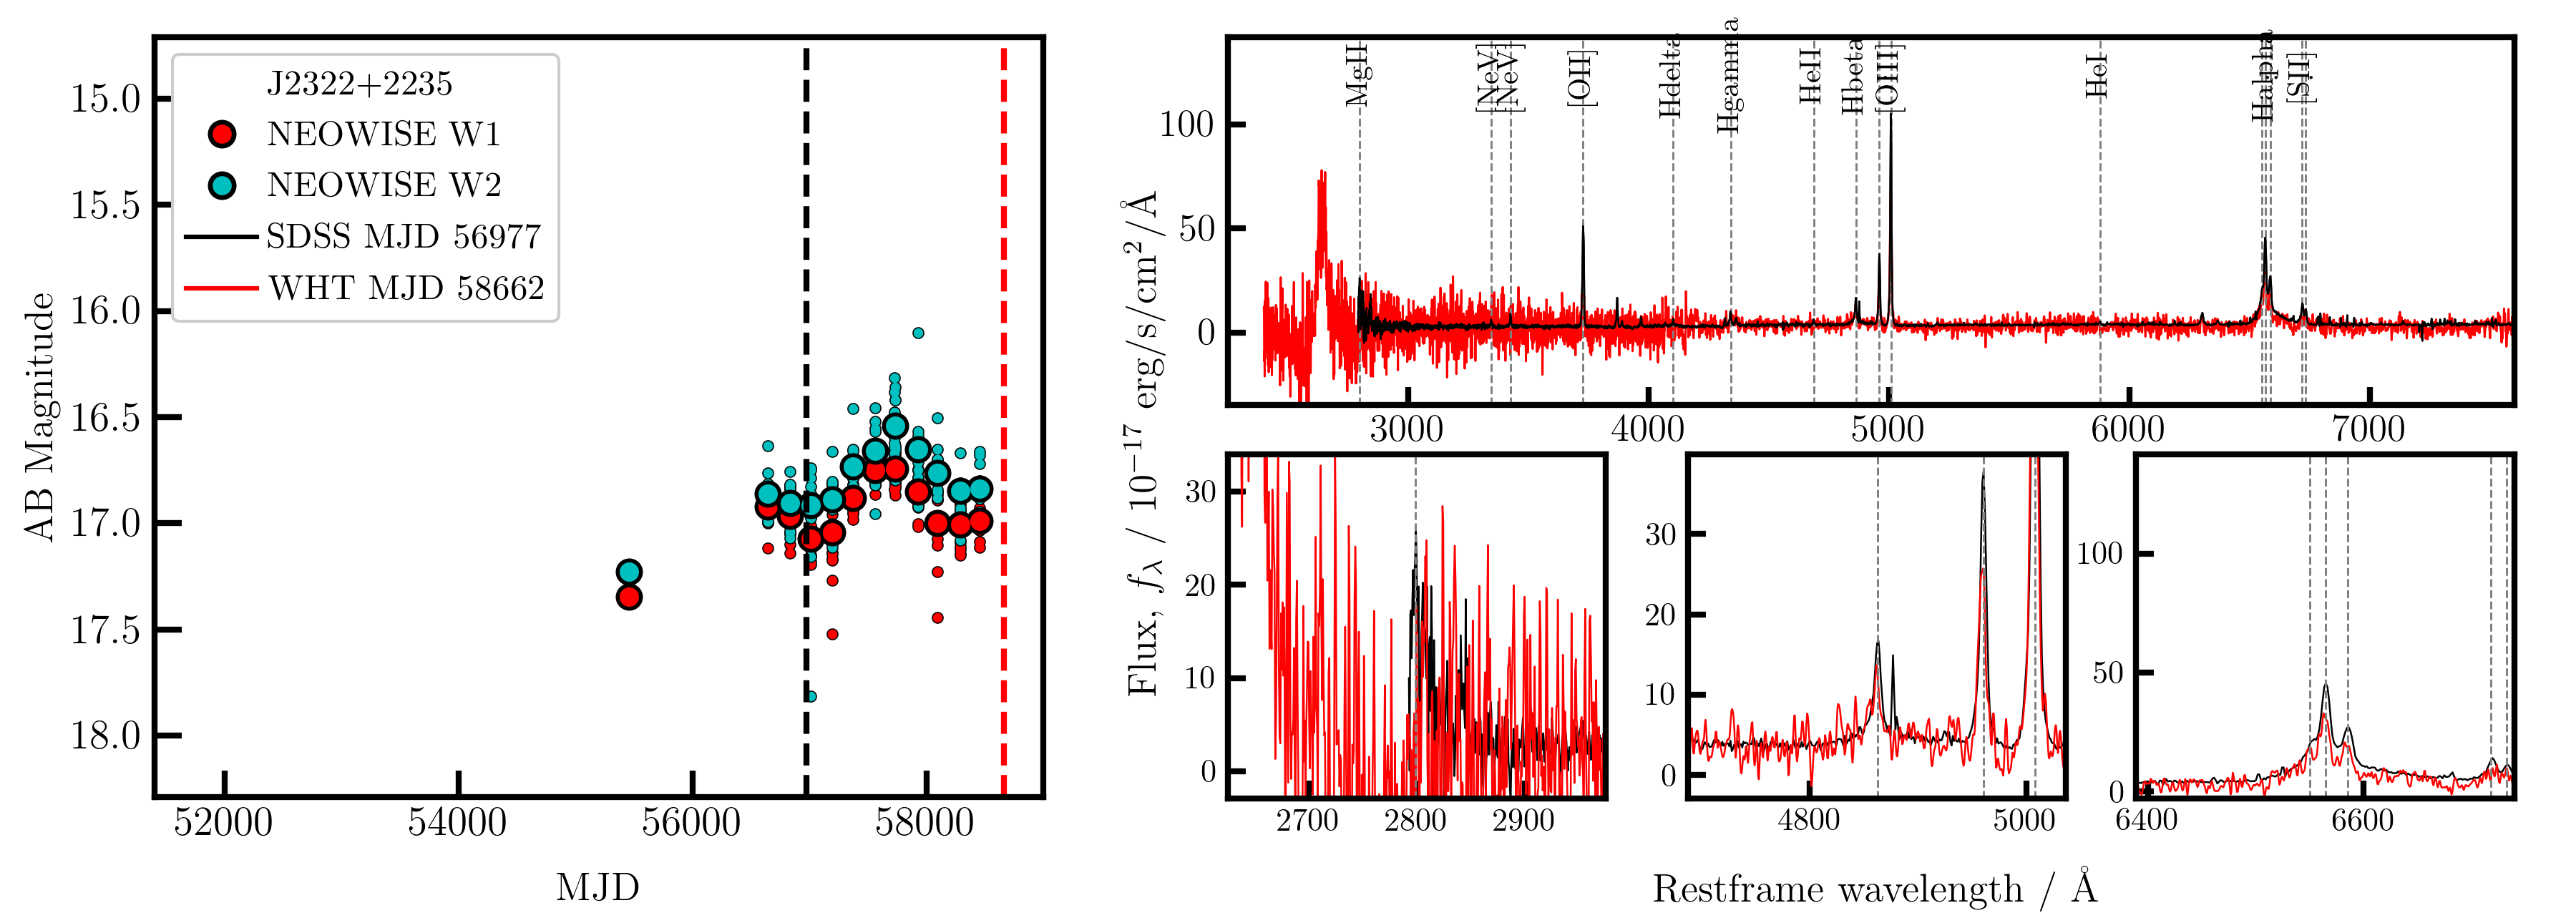
\includegraphics[width=16.7cm, trim=0.0cm 0.05cm 0.2cm 0.1cm, clip]
  {../plots/LCs_and_spectra/J2322+2235_landscape_temp.png}
  \vspace{-12pt}
  \caption[]{}
  \label{fig:all_spectra_f}
\end{figure*}



% Don't change these lines
\bsp	% typesetting comment
\label{lastpage}
\end{document}

